\documentclass{ta-its}
\usepackage{hyperref}
\usepackage{cleveref}
\usepackage{nameref}
\usepackage{multirow}
\usepackage{graphicx}
\usepackage{array}
\usepackage{tabularx}
\usepackage{tabulary}
\usepackage{etoolbox}
\usepackage{listings}
%\usepackage{longtable}
\usepackage{float}
\usepackage{slantsc}
\usepackage{booktabs}% http://ctan.org/pkg/booktabs

\usepackage{caption}
\usepackage{ltxtable} %for long table
% \usepackage{lon} %for long table
\captionsetup[ltxtable]{position=bottom}
\captionsetup[table]{position=bottom}

\usepackage{lipsum} %for lorem ipsum
\usepackage{blindtext} %for lorem ipsum

\usepackage{xcolor} %start packages for colored code listing
\usepackage{upquote} %start packages for colored code listing

\usepackage{enumitem} % for advanced enumerate numberings
\usepackage{scrextend}
% \usepackage{apacite} % for APA citing style

\usepackage[autostyle]{csquotes}
\usepackage{babel}
\usepackage{wrapfig} %untuk wrapfigure?

\usepackage{lscape} %untuk landscape di bagian-bagian tertentu

\newcommand{\mychapter}[2]{
    \setcounter{chapter}{#1}
    \setcounter{section}{0}
    \chapter*{#2}
    \addcontentsline{toc}{chapter}{#2}
}

\newcommand{\mylipsum}
{Dolore blandit mus ultricies justo ultrices, a vel wisi aenean integer lacus vitae, metus lorem nulla, tempor sed odio lacus sit nostra.}

\newcommand{\indentenum}{
    \hspace{\labelwidth}\phantom{\texttt{type}-}
}


\renewcommand{\lstlistingname}{Kode Sumber}
\renewcommand{\lstlistlistingname}{DAFTAR KODE SUMBER}


\colorlet{punct}{red!60!black}
\definecolor{background}{HTML}{EEEEEE}
\definecolor{delim}{RGB}{20,105,176}
\colorlet{numb}{magenta!60!black}
\lstdefinelanguage{json}{
	basicstyle=\normalfont\ttfamily,
	numbers=left,
	numberstyle=\scriptsize,
	stepnumber=1,
	numbersep=8pt,
	showstringspaces=false,
	breaklines=true,
	backgroundcolor=\color{background},
	literate=
	*{0}{{{\color{numb}0}}}{1}
	{1}{{{\color{numb}1}}}{1}
	{2}{{{\color{numb}2}}}{1}
	{3}{{{\color{numb}3}}}{1}
	{4}{{{\color{numb}4}}}{1}
	{5}{{{\color{numb}5}}}{1}
	{6}{{{\color{numb}6}}}{1}
	{7}{{{\color{numb}7}}}{1}
	{8}{{{\color{numb}8}}}{1}
	{9}{{{\color{numb}9}}}{1}
	{:}{{{\color{punct}{:}}}}{1}
	{,}{{{\color{punct}{,}}}}{1}
	{\{}{{{\color{delim}{\{}}}}{1}
	{\}}{{{\color{delim}{\}}}}}{1}
	{[}{{{\color{delim}{[}}}}{1}
	{]}{{{\color{delim}{]}}}}{1}
}
\definecolor{lightgray}{rgb}{0.95, 0.95, 0.95}
\definecolor{darkgray}{rgb}{0.4, 0.4, 0.4}
%\definecolor{purple}{rgb}{0.65, 0.12, 0.82}
\definecolor{editorGray}{rgb}{0.95, 0.95, 0.95}
\definecolor{editorOcher}{rgb}{1, 0.5, 0} % #FF7F00 -> rgb(239, 169, 0)
\definecolor{editorGreen}{rgb}{0, 0.5, 0} % #007C00 -> rgb(0, 124, 0)
\definecolor{orange}{rgb}{1,0.45,0.13}		
\definecolor{olive}{rgb}{0.17,0.59,0.20}
\definecolor{brown}{rgb}{0.69,0.31,0.31}
\definecolor{purple}{rgb}{0.38,0.18,0.81}
\definecolor{lightblue}{rgb}{0.1,0.57,0.7}
\definecolor{lightred}{rgb}{1,0.4,0.5}
% CSS
\lstdefinelanguage{CSS}{
  keywords={color,background-image:,margin,padding,font,weight,display,position,top,left,right,bottom,list,style,border,size,white,space,min,width, transition:, transform:, transition-property, transition-duration, transition-timing-function},	
  sensitive=true,
  morecomment=[l]{//},
  morecomment=[s]{/*}{*/},
  morestring=[b]',
  morestring=[b]",
  alsoletter={:},
  alsodigit={-}
}

% JavaScript
\lstdefinelanguage{JavaScript}{
  morekeywords={typeof, new, true, false, catch, function, return, null, catch, switch, var, if, in, while, do, else, case, break},
  morecomment=[s]{/*}{*/},
  morecomment=[l]//,
  morestring=[b]",
  morestring=[b]'
}

\lstdefinelanguage{HTML5}{
  language=html,
  sensitive=true,	
  alsoletter={<>=-},	
  morecomment=[s]{<!-}{-->},
  tag=[s],
  otherkeywords={
  % General
  >,
  % Standard tags
	<!DOCTYPE,
  </html, <html, <head, <title, </title, <style, </style, <link, </head, <meta, />,
	% body
	</body, <body,
	% Divs
	</div, <div, </div>, 
	% Paragraphs
	</p, <p, </p>,
	% scripts
	</script, <script,
  % More tags...
  <canvas, /canvas>, <svg, <rect, <animateTransform, </rect>, </svg>, <video, <source, <iframe, </iframe>, </video>, <image, </image>, <header, </header, <article, </article
  },
  ndkeywords={
  % General
  =,
  % HTML attributes
  charset=, src=, id=, width=, height=, style=, type=, rel=, href=,
  % SVG attributes
  fill=, attributeName=, begin=, dur=, from=, to=, poster=, controls=, x=, y=, repeatCount=, xlink:href=,
  % properties
  margin:, padding:, background-image:, border:, top:, left:, position:, width:, height:, margin-top:, margin-bottom:, font-size:, line-height:,
	% CSS3 properties
  transform:, -moz-transform:, -webkit-transform:,
  animation:, -webkit-animation:,
  transition:,  transition-duration:, transition-property:, transition-timing-function:,
  }
}

\lstdefinestyle{htmlcssjs} {
  % General design
%  backgroundcolor=\color{editorGray},
  basicstyle=\small\ttfamily,
  % frame=b,
  % line-numbers
  % xleftmargin={0.75cm},
  numbers=left,
  stepnumber=1,
  firstnumber=1,
  numberfirstline=true,	
  % Code design
  identifierstyle=\color{black},
  keywordstyle=\color{blue}\bfseries,
  ndkeywordstyle=\color{editorGreen}\bfseries,
  stringstyle=\color{olive}\ttfamily,
  commentstyle=\color{brown}\ttfamily,
  % Code
  language=HTML5,
  alsolanguage=JavaScript,
  alsodigit={.:;},	
  tabsize=1,
  showtabs=false,
  showspaces=false,
  showstringspaces=false,
  extendedchars=true,
  breaklines=true,
  % German umlauts
  literate=%
  {Ö}{{\"O}}1
  {Ä}{{\"A}}1
  {Ü}{{\"U}}1
  {ß}{{\ss}}1
  {ü}{{\"u}}1
  {ä}{{\"a}}1
  {ö}{{\"o}}1
}
%
\lstdefinestyle{py} {%
language=python,
literate=%
*{0}{{{\color{lightred}0}}}1
{1}{{{\color{lightred}1}}}1
{2}{{{\color{lightred}2}}}1
{3}{{{\color{lightred}3}}}1
{4}{{{\color{lightred}4}}}1
{5}{{{\color{lightred}5}}}1
{6}{{{\color{lightred}6}}}1
{7}{{{\color{lightred}7}}}1
{8}{{{\color{lightred}8}}}1
{9}{{{\color{lightred}9}}}1,
basicstyle=\footnotesize\ttfamily, % Standardschrift
numbers=left,               % Ort der Zeilennummern
%numberstyle=\tiny,          % Stil der Zeilennummern
%stepnumber=2,               % Abstand zwischen den Zeilennummern
numbersep=5pt,              % Abstand der Nummern zum Text
tabsize=4,                  % Groesse von Tabs
extendedchars=true,         %
breaklines=true,            % Zeilen werden Umgebrochen
keywordstyle=\color{blue}\bfseries,
frame=b,
commentstyle=\color{brown}\itshape,
stringstyle=\color{editorOcher}\ttfamily, % Farbe der String
showspaces=false,           % Leerzeichen anzeigen ?
showtabs=false,             % Tabs anzeigen ?
xleftmargin=17pt,
framexleftmargin=17pt,
framexrightmargin=5pt,
framexbottommargin=4pt,
%backgroundcolor=\color{lightgray},
showstringspaces=false     % Leerzeichen in Strings anzeigen ?
}


\definecolor{dkgreen}{rgb}{0,.6,0}
\definecolor{dkblue}{rgb}{0,0,.6}
\definecolor{dkyellow}{cmyk}{0,0,.8,.3}

\lstdefinestyle{php}{
  basicstyle      = \small\ttfamily,
  identifierstyle=\color{black},
  keywordstyle=\color{blue}\bfseries,
  ndkeywordstyle=\color{editorGreen}\bfseries,
  stringstyle=\color{olive}\ttfamily,
  commentstyle=\color{brown}\ttfamily,
  emph            =[1]{php},
  emphstyle       =[1]\color{black},
  emph            =[2]{if,and,or,else,while,function,private,public,protected,<?php,?>},
  emphstyle       =[2]\color{black}\bfseries,
  morecomment=[s]{/*}{*/},
  morecomment=[l]{//},
  }
 %formatting code sources
\newlist{inlinelist}{enumerate*}{1}
\setlist*[inlinelist,1]{
	label={\alph*)},font={\color{red!50!black}\bfseries}
} %enumerate?

\makeatletter
\def\l@lstlisting#1#2{\@dottedtocline{1}{1.5em}{3em}{#1}{#2}}
\makeatother

\raggedbottom

\title{Rancang Bangun Aplikasi \textit{web} Lelang \textit{Online} \textit{(E-Auction)} Berbasis Kerangka Kerja Laravel}{E-Auction Web Application Design and Implementation based on Laravel Framework}{KI141502} 

% \author{Nama Lengkap}{NRP}
\author{Ronauli Silva Natalensis Sidabukke}{5113100142}

% \supervisorOne{Nama Pembimbing Satu}{NIP}
% \supervisorTwo{Nama Pembimbing Dua}{NIP}
\supervisorOne{Rully Soelaiman, S.Kom, M.Kom}{197002131994021001}
\supervisorTwo{Rizky Januar Akbar, S.Kom., M.Eng}{198701032014041001}

% \degree{Nama Gelar}{Bidang Studi}{Program Studi}{Jurusan}{Jurusan (English)}{Fakultas}{Fakultas Singkatan}{Fakultas (English)}
\degree{Sarjana Komputer}{Algoritma Pemrograman}{S1}{Teknik Informatika}{Informatics}{Teknologi Informasi}{FTIf}{Information Technology}

% \time{bulan}{tahun}
\time{Juni}{2017}


\begin{document}
    \maketitle
%    \pagenumbering{}
	\pagenumbering{roman}
    \legalityPaper
    \begin{abstrak}
		Industri e-commerce berkembang dengan pesat di Indonesia, seiring dengan meningkatnya jumlah pengguna internet dan menjamurnya bisnis online atau sering disebut \textit{online shop}. Salah satu jenisnya adalah lelang online, yaitu metode jual beli yang mengintegrasikan mekanisme lelang dengan Internet.
	    \newline
	    \indent Dalam interaksi antara pelaku lelang online (penjual dan pembeli) pasti terjadi kegagalan/ketidakpuasan dalam transaksi lelang online.Berangkat sebuah paper yang membahas mengenai analisa kesalahan dan strategi lewat survey terhadap pengguna aplikasi lelang online di Taiwan, penulis membangun aplikasi lelang online yang disertai dengan tambahan fitur maupun saran dari paper tersebut.
	    \newline 
	    \indent Tidak hanya berdasarkan paper rujukan, penulis juga menganalisa aplikasi \textit{e-commerce} yang umum digunakan di Indonesia baik \textit{user experience} maupun alur transaksi, dan menambahkan beberapa fitur agar lebih sesuai dengan transaksi jual-beli online yang umum di Indonesia. Dengan aplikasi ini, diharapkan kegagalan dalam transaksi online dapat diperbaiki dan membuka peluang lelang online untuk meramaikan industri \textit{e-commerce} di Indonesia.\\
\noindent \textbf{Kata-Kunci}: \textit{lelang online}, \textit{strategi }
\end{abstrak}
    \begin{abstract}
	E-commerce industry is growing rapidly in Indonesia, along with the increasing number of internet users and number of online shops is also growing. One of e-commerce type is online auction, a buy and sell method that integrates auction mechanism and the Internet.\\
	\indent In the interaction between online auction actors (buyers and sellers), inevitable failure/dissatisfaction of online auction transactions sometimes found. Started by analysing paper about online auction application typologies and strategies through an application's users survey, author want to build online auction application along with additional ideas and suggestions from the paper.  \\
	\indent Author also analyzed and considering user experience, design and transaction flow local e-commerce platforms that are commonly used in Indonesia, in purpose to make the application suits Indonesian's users better. Furthermore, author hopes that this applications can reduce/prevent the expected failures in online transactions and open up online auction opportunity to enliven the e-commerce industry in Indonesia.\\
\noindent \textbf{Keyword}: \textit{online auction}, \textit{typologies and strategies}
\end{abstract}
    \mychapter{0}{KATA PENGANTAR}
%   \begin{figure}[h]
%     \centering
%     
\includegraphics[width=0.5\linewidth]{images/bab0/gambarBismillah}
%   \end{figure}
	  Puji Syukur kepada Tuhan yang Maha Esa, atas berkatNya penulis dapat menyelesaikan buku berjudul \textbf{\judul}. 
	  \newline
	  \indent Selain itu, pada kesempatan ini penulis menghaturkan banyak terima kasih kepada pihak-pihak yang tanpa mereka, penulis tidak akan dapat menyelesaikan buku ini dengan baik :
  \begin{enumerate}
  	\item \textbf{\textit{Daddy Jesus}} - atas segala berkat, limpahan karunia, kesempatan dan rancangan jalanNya-lah penulis masih diberi nafas kehidupan, waktu, tenaga dan pikiran untuk menyelesaikan buku ini. \textit{Thank you, Big Daddy.}
    \item \textbf{Papa dan Mama} yang selalu menguatkan, menasehati, dan luar biasa sabar dalam mengingatkan penulis agar tidak lupa menjaga kesehatan dan tidak lupa ke gereja selama masa studi.
    \item \textbf{Yth Bapak Rully Soelaiman} yang mengajarkan penulis \textit{how to think scientifically} juga bimbingan, nasehat, saran dan memberikan penulis sisi pemikiran dan perspektif lain terhadap setiap masalah.
    \item \textbf{Yth Bapak Rizky Januar Akbar} sebagai dosen pembimbing yang memberi bimbingan, saran teknis dan administratif, diskusi dan pemecahan masalah dalam pembuatan dan penulisan buku tugas akhir.
    \item \textbf{Keluarga XL Future Leader Scholarship Camp Batch 5 \& KSE ITS} yang telah menyadarkan, memberikan semangat dan inspirasi untuk terus melanjutkan tugas akhir di saat penulis kehilangan semangat.
    \item \textbf{Keluarga Admin Lab. Pemrograman (2014 - 2017)}, yang telah memberikan penulis banyak pengalaman, pengetahuan dan cerita-cerita untuk dikenang.
    \item  \textbf{Keluarga Pengpro \textit{Furions} dan HMTC Optimasi 2016 }, yang mengajarkan penulis tentang cara berorganisasi, cara berbicara di depan publik, dan banyak lagi. 
    \item Bang Christo yang sudah jadi inspirasi dan semangat kuliah penulis sejak tahun pertama masa studi penulis sampai saat ini.  
    \item \textbf{Keluarga Alumni Budi Mulia Siantar-Surabaya angkatan 2013 }, teman setia disaat suka maupun duka. 
    \item Serta semua pihak yang tidak tertulis - yang telah turut membantu penulis dalam menyelesaikan Tugas Akhir ini.
  \end{enumerate}
  
  \indent Penulis menyadari bahwa Tugas Akhir ini masih memiliki banyak kekurangan. Oleh karena itu, penulis berharap kritik dan saran dari pembaca sekalian untuk memperbaiki buku ini ke depannya.

  \hfill Surabaya, Juli 2017 \\ \\ 


  \hfill Ronauli Silva N. Sidabukke

\cleardoublepage % Mengisi penanda halaman genap yang kosong


    \tableofcontents % Daftar isi
    \listoftables % Daftar tabel
    \listoffigures % Daftar gambar
    \lstlistoflistings % Daftar Kode Sumber

  \mainmatter % Halaman utama, dengan judul BAB X
    \chapter{PENDAHULUAN}
  Pada bab ini akan dipaparkan mengenai garis besar Tugas Akhir yang meliputi latar belakang, tujuan, rumusan dan batasan permasalahan, metodologi pembuatan Tugas Akhir, dan sistematika penulisan.
  \section{Latar Belakang}
  	
	\indent Transaksi jual beli saat ini sudah dapat dilakukan lewat berbagai cara, antara lain menggunakan \textit{e-commerce}, atau lewat \textit{social media}, atau bisa dengan melelang di aplikasi lelang \textit{online}. Sedikit berbeda dengan teknik penjualan di lelang online, karena aplikasi ini dapat diakses oleh banyak orang, tentu saja pelelang (\textit{auctioneer}) tidak terbatas pada ruang lelang saja, tapi bisa berasal dari manapun selama mereka mengakses aplikasi tersebut.  Lelang \textit{online} ini tentu saja mendatangkan banyak manfaat, selain biaya yang lebih efisien dan hemat, dan juga tidak menguras waktu karena siapapun, kapanpun, dimanapun dapat mengajukan penawaran ataupun melelang barangnya tanpa harus pergi ke instansi tertentu dan melakukan lelang dengan cara konvensional.
    \\
    \indent Aplikasi serupa telah banyak, namun banyak aspek yang kurang dalam aplikasi tersebut, seperti informasi dari lelang tidak \textit{reliable} (misal: stok barang ternyata sudah habis), alur proses yang tidak jelas sehingga membingungkan pengguna aplikasi, informasi yang kurang jelas, dan produk yang didapatkan ternyata tidak sesuai dengan informasi pada saat produk dilelang (\textit{bad information}) \cite{ying-feng_kuo_online_2016}.
    \\
    \indent Dan dari masalah teknis aplikasi, beberapa sumber menyatakan bahwa ketidakjelasan alur proses yang kurang diperhatikan oleh para developer aplikasi lelang \textit{online} menjadi beberapa alasan yang kuat mengapa lelang online masih kurang diminati \cite{noauthor_sistem_nodate}.
    \\
	\indent Diharapkan, dengan adanya aplikasi ini, beberapa kelemahan yang masih ada pada aplikasi lelang \textit{online} saat ini dapat diperbaiki, dan juga dapat dapat membantu proses \textit{online} yang ada di Indonesia, dan juga mampu memperbaiki citra aplikasi lelang \textit{online} sehingga mampu meningkatkan minat masyarakat terhadap lelang \textit{online}.
    
  \section{Rumusan Masalah}
    Rumusan masalah yang diangkat dalam tugas akhir ini adalah sebagai berikut: 
    \begin{enumerate}
      \item Bagaimana membangun aplikasi lelang online berbasis web?
      \item Bagaimana rancangan arsitektur aplikasi dan fitur yang menganalisa kelemahan aplikasi serupa dan strategi penyelesaian sesuai dengan paper acuan \cite{ying-feng_kuo_online_2016}?
    \end{enumerate}

  \section{Batasan Masalah}
  	\label{batasan-masalah}
    Dari permasalahan yang telah diuraikan di atas, terdapat beberapa batasan masalah pada tugas akhir ini, yaitu:
    \begin{enumerate}
      \item Aplikasi berbasis web dengan bahasa pemrograman PHP.
      \item Aplikasi berbasis kerangka kerja Laravel.
      \item Basis data yang digunakan adalah PostgreSQL.
      \item Aplikasi tidak mencakup proses pembayaran.
    \end{enumerate}

  \section{Tujuan}
  \label{tujuan}
    Tujuan dari pengerjaan Tugas Akhir ini adalah: 
    \begin{enumerate}
      \item Membangun aplikasi lelang online berbasis web yang lebih kredibel sesuai dengan paper yang dijadikan acuan pada tugas akhir ini. 
    \end{enumerate}
    \chapter{LANDASAN TEORI}{}
  \section{Lelang Daring / Lelang \textit{Online}}
   Lelang adalah proses membeli dan menjual barang atau jasa dengan cara menawarkan kepada penawar, menawarkan tawaran harga lebih tinggi, dan kemudian menjual barang kepada penawar harga tertinggi. Dalam teori ekonomi, lelang mengacu pada beberapa mekanisme atau peraturan perdagangan dari pasar modal. \\
	Sementara lelang daring atau lelang melalui internet muncul seiring dengan perkembangan internet. Barang atau jasa yang diperjualbelikan dipasang di situs dan peserta lelang dapat mengikuti acara lelang secara daring. Perusahaan lelang yang berhasil menggunakan sarana internet salah satunya adalah \textit{Ebay} . Di Indonesia, lelang melalui internet (online) sudah dipelopori oleh pemerintah dengan situs lelang online yang dapat diakses melalui website resmi \href{https://www.lelangdjkn.kemenkeu.go.id}{Kemenkeu} \cite{wikipedia_lelang_2016} . 
    Berikut adalah beberapa istilah yang ada dalam lelang online :
    \begin{enumerate}
	\item BID atau \textit{Bidding}, artinya : Menawarkan
    \item BIN (\textit{Buy In Now}) artinya : Beli sesuai harga yang telah ditawarkan penjual
    \item INC (\textit{Increment}) artinya : Minimum kenaikan \textit{bid} setelah \textit{bid} sebelum nya \cite{noauthor_arti_nodate}
    \end{enumerate}
    
    \section{PostgreSQL}
    PostgreSQL adalah sebuah produk \textit{database} relasional yang termasuk dalam kategori \textit{free open source software} (\textit{FOSS}). 
	PostgreSQL terkenal karena fitur-fitur yang advanced dan pendekatan rancangan modelnya menggunakan paradigma \textit{object-oriented}, sehingga sering dikategorikan sebagai \textit{Object Relational Database Management System} (ORDBMS).
    Beberapa fitur PostgreSQL adalah sebagai berikut :
    \begin{enumerate}
    \item \textit{Inheritance}, dimana satu table dapat diturunkan model dan beberapa karakteristik dari table lainnya.
    \item \textit{Multi-Version Concurrency Control} dimana user diberi data snapshot ketika suatu perubahan dilakukan sampai commit.
    \item \textit{Rules} , dimana suatu \textit{query} DML yang dikirimkan ke server akan mengalami penulisan ulang (\textit{rewrite}). Ini terjadi sebelum diproses oleh \textit{query planner}.
    \item dan berbagai fitur lainnya \cite{noauthor_postgresql_nodate}
    \end{enumerate}
    
  \section{Redis}
    Redis adalah \textit{open source}, struktur data yang ditempatkan di memori, digunakan sebagai \textit{database}, \textit{cache} dan \textit{message broker}. Redis mendukung struktur data seperti \textit{string, sets, hash, lists} dan \textit{sorted sets}. Sama seperti cache, setiap key diisi oleh value. Tapi kelebihannya, Redis bisa digunakan untuk melakukan operasi dari value tersebut. Cara terbaik untuk memahami redis adalah membuat model aplikasi tanpa memikirkan bagaimana caranya untuk menyimpan data di dalam \textit{database} \cite{yudana_redis_2015}.

  \section{Node.js}
  Node.js adalah platform perangkat lunak pada sisi-server dan aplikasi jaringan. Ditulis dengan bahasa javascript dan bisa dijalankan pada Windows, Mac OS X dan Linux tanpa perubahan kode program. Node.js memiliki pustaka server HTTP sendiri sehingga memungkinkan untuk menjalankan webserver tanpa menggunakan program webserver seperti Apache atau Lighttpd \cite{noauthor_node.js_2014}.
  
  \section{Socket.io}
	Socket.io adalah \textit{library} Javascript untuk aplikasi web yang bersifat \textit{realtime}. Socket.io menjembatani antara komunikasi dua arah antara \textit{web} \textit{clients} dan \textit{server}. Socket.io terbagi menjadi dua bagian, yaitu \textit{client}-\textit{side} \textit{library} yang berjalan di browser client, dan \textit{server}-\textit{side} \textit{library} yang menggunakan Node.js. Kedua komponen tersebut mempunyai API yang sama. Seperti Node.js, Socket.io juga bersifat \textit{event}-\textit{driven}. Socket.IO menggunakan protokol \textit{websocket} dengan \textit{polling} sebagai opsi \textit{fallback}. Meskipun Socket.IO merupakan ‘pembungkus’ untuk soket web, namun ia memiliki banyak fitur, antara lain broadcast ke banyak soket, dan I/O yang asinkronus \cite{noauthor_socket.io_2016}.
    
    \section{Laravel}
    Laravel adalah \textit{framework} PHP yang dikembangkan pertama kali oleh Taylor Otwell. Walaupun termasuk baru, namun komunitas pengguna laravel sudah berkembang pesat dan mampu menjadi alternatif utama dari sejumlah \textit{framework} besar seperti CodeIgniter dan Yii. Laravel oleh para \textit{developer} disetarakan dengan CodeIgniter dan FuelPHP namun memiliki keunikan tersendiri dari sisi \textit{coding}. Laravel memiliki beberapa keunggulan, diantaranya :
\begin{enumerate}
\item Sintaks yang sederhana dan \textit{programmer}-\textit{fiendly}
\item Tersedia \textit{generator} yang canggih dan memudahkan, Artisan CLI
\item Fitur \textit{Schema} \textit{Builder} untuk berbagai \textit{database}
\item Fitur \textit{Migration} dan \textit{Seeding} untuk berbagai \textit{database}
\item Fitur \textit{Query} \textit{Builder} yang powerful
\item Eloquent ORM (\textit{Object} \textit{Relational} \textit{Mapping})
\item Fitur pembuatan \textit{package} dan \textit{bundle}
\item \textit{Dependency} \textit{Injection} \cite{a}
\end{enumerate}

	\section{Protokol SMTP}
    
	\section{JSON Web Token}
    
   \section{Service Worker}
   
   \section{Repository Pattern}
   
   \section{Concurrency}
   
   \section{Transaction Isolation}
   
   \section{Script Testing}
   
   \section{Laravel Dusk}
   
   


    \chapter{ANALISA DAN PERANCANGAN SISTEM}  
  \section{Analisa}

	%Requirement Analysis
	\subsection{\textit{Requirement Analysis}}
	\subsubsection{Fungsionalitas Dasar}

Aplikasi Lelang Online berbasis Web yang diberi nama \textbf{Lelangapa} adalah sebuah \textit{online auction web} yang dibangun berdasarkan paper rujukan utama, dengan fitur-fitur utama sebagai berikut:

\begin{enumerate}
	\item \textbf{Registrasi ke dalam sistem}
	\item \textbf{Login ke dalam sistem}
	\item \textbf{Mendaftarkan barang untuk dilelang} \\
	Pengguna dapat mendaftarkan barangnya untuk dijual dan dilelang. Selain itu, pengguna dapat menentukan harga awal dan batas waktu lelang pada saat mendaftarkan barangnya.
	\item \textbf{Memperbarui barang yang dilelang} \\
	Pengguna dapat memperbarui informasi mengenai barang yang dilelang, seperti nama barang, menambah foto deskripsi barang, atau menambah waktu lelang.
	\item \textbf{Melihat informasi barang yang dilelang} \\
	Pengguna dapat melihat detail informasi barang yang sedang dilelang – seperti foto barang, riwayat penawaran harga barang lelang, sisa waktu penawaran, deskripsi barang, dsb.
	\item \textbf{Melihat informasi riwayat lelang} ( Siapa saja yang sudah mengajukan penawaran dan harga yang ditawarkan )
	\item \textbf{Mengajukan penawaran harga untuk barang yang dilelang / Menjadi auctioneer} \\
	Selain menjadi auctioneer, pengguna juga dapat menawarkan harga terhadap barang-barang yang didaftarkan oleh pengguna lain.
	\item \textbf{Mendapatkan pemberitahuan jika penawaran harga dikalahkan dengan harga lebih tinggi} \\
	Pengguna mendapatkan pemberitahuan jika pengguna sedang mengikuti pelelangan barang, dan ada penawaran harga yang lebih tinggi dari penawaran oleh pengguna tersebut, sehingga pengguna dapat mengikuti perkembangan harga dari barang yang dilelang.
	\item \textbf{Mengikuti / follow barang yang sedang dilelang dan mendapatkan pemberitahuan jika barang tersebut }\\
	Jika pengguna sedang tidak ingin melelang barang namun ingin tetap mengetahui informasi dari suatu barang lelang, pengguna dapat mengikuti feed/berita dari barang tersebut.
	\item \textbf{Mendapatkan pemberitahuan jika memenangkan lelang atau tidak.}\\
	Jika pengguna mengajukan penawaran harga terhadap suatu barang, maka pengguna akan mendapatkan pemberitahuan pada saat batas waktu lelang selesai, apakah pengguna tersebut memenangkan proses lelang tersebut atau tidak.
	\item \textbf{Saling berkirim pesan singkat/chat kepada auctioneer/penawar harga }\\
	Untuk saling bertukar informasi mengenai barang yang sedang dilelang, auctioneer dan penawar harga dapat saling berkirim pesan singkat.
	\item \textbf{Melihat riwayat penawaran harga lelang }\\
	Pengguna dapat melihat barang riwayat penawaran harga yang diberikan oleh pengguna tersebut terhadap semua barang yang pernah dia lelang.
	\item \textbf{Melihat riwayat barang yang dilelang }\\
	Pengguna dapat melihat riwayat barang yang pernah ditawar harganya/diberikan penawaran harga.
	\item \textbf{Memberi review tentang pengguna lain sebagai auctioneer dan atau sebagai penawar harga }\\
	Pengguna dapat memberikan komentar/testimoni berdasarkan pengalaman bertransaksi/penawaran harga dengan pengguna lainnya, baik pengalaman memuaskan ataupun pengalaman buruk.
	\item\textbf{ Melihat review mengenai seorang pengguna }\\
	Selain memberikan review, pengguna dapat melihat review seorang pengguna.
	\item \textbf{Memblok pengguna sebagai auctioneer }\\
	Auctioneer dapat memblok pengguna agar pengguna tersebut tidak memberikan penawaran harga terhadap barang yang sedang ia lelang. Hal ini bisa saja karena review/testimoni pengguna tersebut buruk atau karena alasan lainnya.
	\item \textbf{Mencari barang yang dilelang dengan keyword tertentu}
\end{enumerate} %checked
	
    \subsubsection{Analisa Paper Rujukan}
	    \label{analisa-paper-rujukan}
	    Dengan perkembangan teknologi, perlahan kebiasaan manusia berubah. Termasuk juga dalam perdagangan, dimana transaksi jual beli barang tidak lagi harus melalui tatap muka. Penjualan online saat ini sudah dapat dilakukan lewat berbagai cara, antara lain menggunakan e-commerce, atau posting di social media, atau bisa juga dengan melelang di aplikasi lelang online. Sedikit berbeda dengan teknik penjualan di lelang online, karena aplikasi ini dapat diakses oleh banyak orang, tentu saja pelelang (\textit{auctioneer}) tidak terbatas pada ruang lelang saja, tapi bisa berasal dari manapun selama mereka mengakses aplikasi tersebut.  Lelang online ini tentu saja mendatangkan banyak manfaat, selain biaya yang lebih efisien dan hemat, dan juga tidak menguras waktu karena siapapun, kapanpun, dimanapun dapat mengajukan penawaran ataupun melelang barangnya tanpa harus pergi ke instansi tertentu dan melakukan lelang dengan cara konvensional.\\
		\indent Bercermin terhadap aplikasi \textit{e-commerce} yang telah ada, masalah yang paling sering dialami adalah ketidakpuasan pengguna. Salah satu indikator bahwa suatu perusahaan dikatakan memiliki ketidakpuasan pelanggan adalah karena kegagalan dalam pelayanannya. Seorang pelanggan sangat mungkin memutuskan untuk komplain setelah mengalami ketidakpuasan terhadap layanan suatu perusahaan, dan jika tidak ditangani dengan baik, hal ini bisa berakibat fatal terhadap reputasi dan kepercayaan pengguna terhadap aplikasi tersebut. \\
		\indent Oleh karena itu, sebuah paper mengangkat topik ini khusus dalam bidang aplikasi lelang online, menganalisa kegagalan dan ketidakpuasan pengguna, beserta solusi-solusi yang ditawarkan oleh pengguna aplikasi untuk memperbaiki kegagalan pelayanan tersebut. 
		
	  \begin{figure}[H]
        \centering
        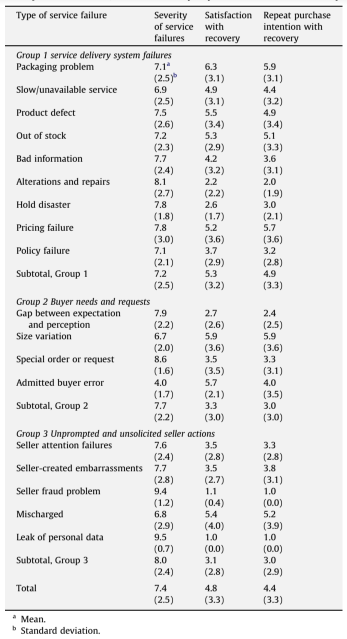
\includegraphics[height=.5\textheight]{images/bab3/Fatalitas-Kegagalan-Ecommerce.png}
        \caption{Fatalitas kegagalan dalam aplikasi Lelang Online, Kepuasan terhadap Perbaikan Pelayanan dan \textit{Repeat Purchase Intention} setelah Perbaikan Layanan}
        \label{severity-failures}
      \end{figure}
      
      \indent Dalam gambar diatas, dijabarkan beberapa jenis kegagalan yang pernah dialami oleh pengguna aplikasi serta fatalitas/pengaruh buruk kegagalan tersebut terhadap kepercayaan pengguna. 
      
	  \begin{figure}[H]
        \centering
        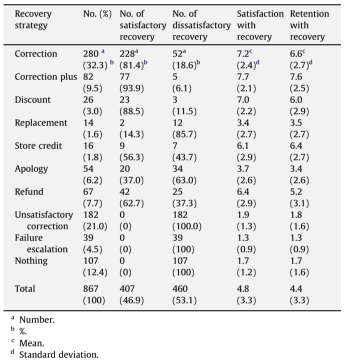
\includegraphics[width=\linewidth]{images/bab3/Solusi-Perbaikan-Ketidakpuasan.png}
        \caption{Kategori Perbaikan terhadap Kegagalan Pelayanan Lelang Online}
        \label{service-recovery-strategies}
      \end{figure}
      
      \indent Maka berdasarkan hasil analisa tersebut, fitur-fitur yang perlu ditambahkan selain daripada fitur dasar aplikasi lelang online adalah sebagai berikut :
      \begin{enumerate}
      \item Fitur chatting, untuk mengurangi kemungkinan \textit{Bad Information} dimana ekspektasi dan persepsi terhadap barang yang dilelang antara pembeli dan penjual tidak sama dan \textit{Special Needs}, 
      \item Fitur pemberian kupon voucher (\textit{Discount and Correction Plus}) yang bisa berupa \textit{free shipping} atau \textit{discount}.
      \end{enumerate}
   %checked
	\subsection{\textit{Bussiness Aspects of Software Engineering}}
	
	Lelang merupakan salah satu metode pertukaran barang dan jasa dengan metode penetapan harga yang berbeda dengan perdagangan. Oleh karena itu, lelang juga termasuk dalam kategori bisnis. Yang menarik adalah, ketika bisnis digabungkan dengan teknologi atau yang sering disebut \textit{e-commerce}, hal yang sekedar pertukaran barang bertransformasi menjadi sebuah sistem interaktif yang kompleks dimana tujuan utamanya adalah menarik pengunjung/pengguna untuk menyelesaikan sebuah transaksi. Hal ini tentu sangat krusial, penting, dan tertantang untuk menyelesaikannya. \\
	\indent Dalam mencapai kesuksesan dan tingkat kompetitif yang tinggi, haruslah menyediakan layanan dengan kesan \textit{user experience (UX)} yang positif bagi para penggunanya. Morville  \cite[p.~27]{a-set-of-heuristics-2014} , dalam studi yang dilakukannya, menyebutkan bahwa UX tercakup dalam 7 aspek esensial, yaitu \begin{enumerate}[label=\alph*.]
		\item \textit{useful}
		\item \textit{usable}
		\item \textit{findable}
		\item \textit{desirable}
		\item \textit{accessible}
		\item \textit{credible}.
		\end{enumerate}
	
	\indent Hasil-hasil temuan penting yang menarik dalam pengaruh \textit{user experience}, adalah sebagai berikut dikutip dari sebuah sumber adalah sebagai berikut:
	\begin{enumerate}[label=\alph*.]
		\item \textit{User tend to leave if a page loads more than 3 seconds};
		\item \textit{79\% of users won't return if the web's performance and experience is poor};
		\item \textit{44\% of users will tell the poor experiences to their friends}.
	\end{enumerate}
	
	\indent Selain dari faktor \textit{user experience} dan \textit{performance}, beberapa hal yang menjadi poin penting dan menarik dalam beberapa studi yang terkait adalah sebagai berikut:
	\begin{enumerate}[label=\alph*]
		\item \textit{Familiarity} - yang dapat didefinisikan sebagai tingkat familier atau kesamaan dengan sistem sejenis ternyata dapat membangun \textit{trust} sehingga mensugesti pengguna untuk menyelesaikan transaksi yang dilakukan;
		\item \textit{Usability} yang memudahkan pengguna dalam menyelesaikan transaksi; dan
		\item Aspek-aspek psikologi seperti pemilihan warna, penggunaan \textit{icon} yang sesuai, seperti \textit{icon} gembok pada halaman pembayaran ternyata dapat mengesankan \textit{security} pada pengguna.
	\end{enumerate}
	
	
	\begin{figure}[H]
		\centering
		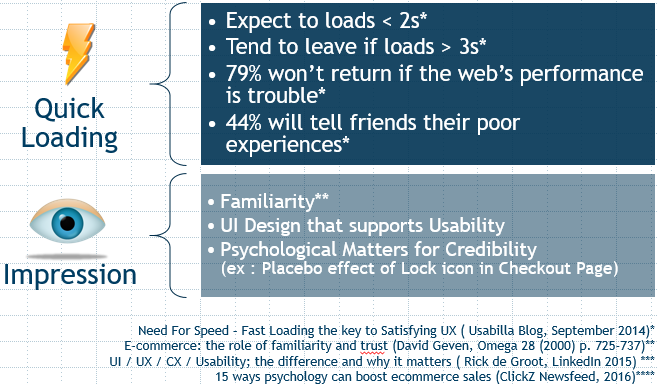
\includegraphics
		[width=\textwidth]
		{images/bab3/analisa/user-centered.png}
		\caption{Visualisasi aspek bisnis dalam \textit{software engineering}}
		\label{user-centered-analysis}
	\end{figure}
	
	\indent Dari hasil temuan ini, dapat disimpulkan bahwa \textit{user experiences, performances, usability} dan psikologi memiliki pengaruh besar dalam kesuksesan lelang online dalam menarik hati para penggunanya. Hal ini akan mempengaruhi definisi kebutuhan fungsionalitas yang akan dibahas dalam subbab \ref{keb-fungsional}.
		
		
		 
	  \subsubsection{Spesifikasi Kebutuhan Fungsional}
  \label{keb-fungsional}
	Berdasarkan deskripsi umum sistem pada subbab \ref{deskripsi-umum-app}, maka dapat disimpulkan bahwa kebutuhan fungsional dari aplikasi lelang online, yang dipaparkan dalam Tabel \ref{tabel-fungsional}.

  \LTXtable{\textwidth}{tables/03b/functional.tex}	
   %checked
	
  \subsection{Spesifikasi Kebutuhan Non-Fungsional}
  
  Kebutuhan non-fungsional yang harus dipeuhi oleh aplikasi ini berhubungan dengan faktor-faktor sebagai berikut:

	\LTXtable{\textwidth}{tables/03b/nonfunctional.tex}	
  
  \newpage %checked
	\subsubsection{\textit{Bussiness Modelling Workflow}} 
	\subsection{Spesifikasi Kasus Penggunaan}
	Kasus penggunaan disini dimaksudkan untuk menurunkan kebutuhan fungsional yang telah dispesifikasikan sebelumnya pada tabel \ref{tabel-fungsional} sebelumnya.\\
	Daftar kasus Penggunaan dapat dilihat pada \ref{kasus-penggunaan}.
	
	\LTXtable{\textwidth}{tables/03c/kasus_penggunaan.tex}
	\begin{figure}[H]
		\centering
		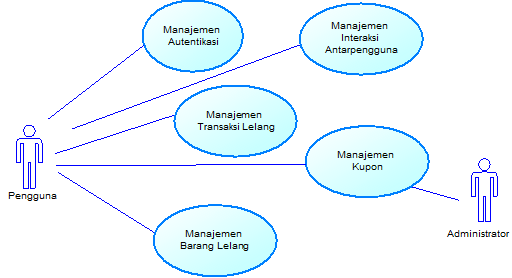
\includegraphics
		[width=\textwidth]
		{images/bab3/usecasediagram/ucd-main.png}
		\caption{Diagram Kasus Penggunaan Aplikasi}
		\label{ucd.main}
	\end{figure}
	
	Selanjutnya, akan dijabarkan masing-masing Spesifikasi Kasus Penggunaan untuk semua  Kasus Penggunaan yang telah dijabarkan diatas.
	
	\input{Chapters/Details/bab3/3cxx/KP01}
	
	\input{Chapters/Details/bab3/3cxx/KP02}
	
	\input{Chapters/Details/bab3/3cxx/KP03}
	
	\input{Chapters/Details/bab3/3cxx/KP04}
	
%	\input{Chapters/Details/bab3/3cxx/KP05}
	
	\input{Chapters/Details/bab3/3cxx/KP06}







 %checked
	
	
	%Technical Analysis
	\subsection{\textit{Technical Analysis}}
	\subsection{Identifikasi Komponen Fundamental}
	Berdasarkan Bab Analisa, dapat diidentifikasi dan divisualisasikan pada Gambar \ref{fundamental-component} yaitu komponen-komponen penting dalam pembuatan aplikasi sebagai berikut:
	\begin{enumerate}
		\item Web Server 
		\item Mekanisme penyimpanan data (\textit{database} dan \textit{data storage})
		\item \textit{User Interface} sebagai media terhadap \textit{end-user}
		\item Mekanisme Asinkronus untuk mengakomodasi fitur \textit{realtime}
	\end{enumerate}
	
	\begin{figure}[H]
		\centering
		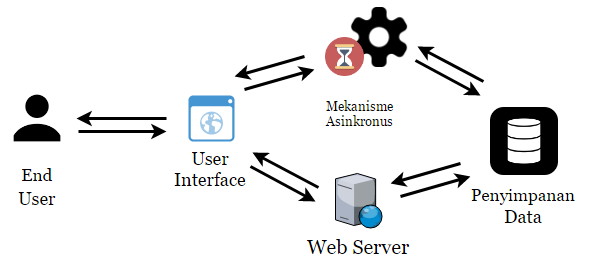
\includegraphics
		[width=\textwidth]
		{images/bab3/buku/basic_architecture.png}
		\caption{Arsitektur dasar yang dibutuhkan untuk membangun aplikasi}
		\label{fundamental-component}
	\end{figure}
	
	
	

	\subsection{\textit{Arsitektur Fundamental}}
	
\subsection{\textit{Technology Options}}
\label{tech-options}

	Pada subbab sebelumnya, penulis sudah memaparkan arsitektur dasar yang dibutuhkan dalam rancang bangun aplikasi. Terkait dengan arsitektur dasar tersebut, banyak pilihan teknologi yang dapat mengimplementasikan arsitektur tersebut. Dalam pemaparan selanjutnya, akan dijelaskan alasan penulis \textit{best practice} dalam pemilihan teknologi yang digunakan, didasarkan pada \textit{best practices} dan pengalaman-pengalaman penulis. Keterkaitan dengan aspek-aspek yang dijelaskan sebelumnya pada subbab \ref{tech-analysis}.
	
	\subsubsection{\textsc{Nginx} sebagai Web Server}
		\begin{itemize}
			\item Kelebihan
				\begin{enumerate}
					\item Konfigurasi yang lebih \textit{friendly} dan terstruktur
					\item Ketersediaan fitur yang lengkap \& krusial (\textit{reverse proxy}, memungkinkan skalabilitas \& \textit{load balancing})
					\item \textit{Learning-gap} yang kecil terhadap pengalaman penulis/sudah familiar
				\end{enumerate}
			\item Opsi lainnya
				\begin{enumerate}
					\item Apache2:  Fiturnya kurang lengkap
					\item Node.js:  \textit{Learning-gap} yang besar bagi penulis/belum familiar
					\item Python:  Belum Familiar, dan perlu eksplorasi fitur lebih dalam
				\end{enumerate}
		\end{itemize}
	
	\subsubsection{\textsc{PostgreSQL} untuk Penyimpanan Data}
	\begin{itemize}
		\item Kelebihan
		\begin{enumerate}
			\item \textit{Learning gap} yang kecil
			\item Stabil karena telah digunakan dan dikembangkan oleh banyak \textit{developer} selama bertahun-tahun
		\end{enumerate}
		\item Opsi lainnya
		\begin{enumerate}
			\item SQL Server:  Instalasi yang kompleks, penggunaan \textit{resource} yang cukup besar
		\end{enumerate}
	\end{itemize}
	
	\subsubsection{\textsc{MongoDB} untuk Penyimpanan Data Nontansaksional}
		\begin{itemize}
			\item Kelebihan
			\begin{enumerate}
				\item \textit{Learning curve} yang mudah/sintaksnya kurang lebih sama dengan sintaks \textit{database} transaksional pada umumnya
				\item Performa yang cepat karena menggunakan BSON
				\item Fitur yang lengkap untuk \textit{sustainability} aplikasi seperti (Replikasi, Sharding, dll)
				\item \textit{Handling} terhadap data yang sangat besar yang cukup bagus, cocok untuk data yang masif seperti \textit{chatting}.
			\end{enumerate}
			\item Opsi lainnya
			\begin{enumerate}
				\item Redis:  Cepat, namun penyimpanan dilakukan di RAM sehingga lebih cocok untuk penyimpanan \textit{auth session}, bukan untuk penyimpanan data yang sifatnya masif
				\item Cassandra:  \textit{Learning-gap} yang besar, namun fiturnya lengkap untuk \textit{data mining}
			\end{enumerate}
		\end{itemize}
		
		
	\subsubsection{\textsc{CDN} sebagai \textit{Assets Sources}}
		\begin{itemize}
			\item Kelebihan
			\begin{enumerate}
				\item Akses cepat karena besar kemungkinan asset tersebut telah di\textit{cache} sebelumnya dalam browser pengguna
				\item Mengurangi \textit{bandwith} server
				\item Telah dioptimasi oleh pengembang masing-masing asset.
			\end{enumerate}
			\item Opsi lainnya
			\begin{enumerate}
				\item Disimpan dalam server: Mengurangi \textit{bandwith} server (\textit{cost} meningkat)
			\end{enumerate}
		\end{itemize}
		
	\subsubsection{\textsc{AWS S3} untuk \textit{Content Growth Scalability}}
	\begin{itemize}
		\item Kelebihan
		\begin{enumerate}
			\item \textit{Benefit} yang sangat \textit{krusial}:  keamanan, skalabilitas, \textit{availability} - karena sudah di\textit{handle} langsung oleh pengembang \textit{cloud computing} yang ahli di bidangnya
			\item Perkembangan jumlah konten yang akan disimpan (gambar barang yang diupload pengguna)  tentunya bersifat sangat masif, sehingga tidak mungkin disimpan dalam server
		\end{enumerate}
		\item Opsi lainnya
		\begin{enumerate}
			\item Disimpan dalam server: Mengurangi performa server karena sifatnya yang memakan \textit{resource} cukup banyak, dan menambah \textit{cost} untuk \textit{upgrade server storage}
		\end{enumerate}
	\end{itemize}
	
	\subsubsection{\textsc{SendGrid} untuk SMTP Relay}
	\begin{itemize}
		\item Kelebihan
		\begin{enumerate}
			\item Konfigurasi yang mudah
			\item Dokumentasi yang cukup lengkap dan mudah ditemukan
			\item Fitur yang lengkap
			\item Adanya \textit{free storage} dari akun Github Student Pack penulis
		\end{enumerate}
		\item Opsi lainnya
		\begin{enumerate}
			\item MailChimp:  Dokumentasi kurang lengkap, tidak ada \textit{free storage} untuk akun penulis
		\end{enumerate}
	\end{itemize}
	
	\subsubsection{\textsc{Vue.js} untuk \textit{Workloads Sharing}}
		\begin{itemize}
			\item Kelebihan
			\begin{enumerate}
				\item \textit{Learning-gap} relatif kecil dibandingkan \textit{Javascript tools} lainnya, karena didesain khusus untuk Laravel
				\item Adanya program utilitas (webpack) yang membuat performa Vue.js jauh lebih cepat
				\item Logika aplikasi dapat di\textit{obfuscate} dengan webpack (\textit{embedded} dalam Laravel)
			\end{enumerate}
			\item Opsi lainnya
			\begin{enumerate}
				\item React:  \textit{Learning gap} dan \textit{learning curve} yang sangat besar untuk penulis
				\item jQuery:  tidak efektif karena \textit{code smells} yang ditimbulkan cukup banyak
			\end{enumerate}
		\end{itemize}
		
	\subsubsection{\textsc{Socket.io} untuk Mekanisme Asinkronus}
		\begin{itemize}
			\item Kelebihan
			\begin{enumerate}
				\item \textit{Learning-gap} relatif kecil dibandingkan \textit{Javascript tools} lainnya, karena didesain khusus untuk Laravel
				\item Adanya program utilitas (webpack) yang membuat performa Vue.js jauh lebih cepat
				\item Logika aplikasi dapat di\textit{obfuscate} dengan webpack (\textit{embedded} dalam Laravel)
			\end{enumerate}
			\item Opsi lainnya
			\begin{enumerate}
				\item React:  \textit{Learning gap} dan \textit{learning curve} yang sangat besar untuk penulis
				\item jQuery:  tidak efektif karena \textit{code smells} yang ditimbulkan cukup banyak
			\end{enumerate}
		\end{itemize}		
		
	\subsubsection{\textsc{JWT} untuk Keamanan Soket}
		\begin{itemize}
			\item Kelebihan
			\begin{enumerate}
				\item \textit{Library support} yang lengkap untuk komponen-komponen lainnya
				\item Efektif dan efisien karena tidak ada \textit{query} ke database untuk autentikasi
			\end{enumerate}
			\item Opsi lainnya
			\begin{enumerate}
				\item \textit{Query} ke \textit{database} secara konvensional:  Sifat koneksi soket yang masif akan sangat memberatkan \textit{database} jika setiap kali ada koneksi baru, harus melakukan \textit{query database} sehingga tidak efektif
				\item \textit{Session caching} dengan Redis:  \textit{Learning gap} yang besar
			\end{enumerate}
		\end{itemize}
		
	\subsubsection{\textsc{Laravel Dusk} untuk \textit{Functionality Testing Script}}
		\begin{itemize}
			\item Kelebihan
			\begin{enumerate}
				\item \textit{Learning gap} yang kecil karena didesain sefamiliar mungkin dengan Laravel
			\end{enumerate}
			\item Opsi lainnya
			\begin{enumerate}
				\item Selenium:  \textit{Learning curve} yang besar
				\item Phantom.js:  \textit{Learning curve} yang besar
			\end{enumerate}
		\end{itemize}
	
	

	
	
	
	\subsection{\textit{Summary}}



\subsection{Analisa \textit{User Experience} dari E-Commerce di Indonesia}
\label{alasan-ux-ecommerce-indonesia alasan-app-serupa}
Selama masa pengerjaan aplikasi, penulis sering menganalisa dan memperhatikan kebiasaan-kebiasaan yang umum di website \textit{e-commerce} di Indonesia. Salah satu yang paling sering dianalisa oleh penulis adalah adalah situs Tokopedia.
\\
\indent Beberapa hal yang dianalisa penulis adalah:
\begin{enumerate}
	\item Halaman yang muncul bukanlah eagerloading, tapi \textit{lazy loading}\\
	\indent Ini adalah solusi cerdas untuk mengakali \textit{delay loading item} yang sudah pasti jumlahnya sangat banyak (maka butuh \textit{query} yang tentunya memakan waktu cukup lama), namun juga memainkan faktor psikologi / \textit{user behaviour} pengguna dengan membiarkan pengguna melihat tahap demi tahap halaman 'diisi'.
	\item \textit{User Interface} yang sederhana dan pemilihan warna yang \textit{soft}
\end{enumerate}
Dari 2 poin tersebut, sebisa mungkin saya adaptasi ke dalam aplikasi Lelang Online ini.

\subsection{Analisa Keamanan pada koneksi Soket}
\label{alasan-socket.io}
Untuk mengakomodasi fitur yang bersifat \textit{realtime}, dibutuhkan koneksi ke soket secara terus menerus. Hal ini tentu dapat menjadi sasaran empuk \textit{security} karena jika tidak diamankan, maka dapat menjadi peluang besar bagi para pihak yang tidak berkepentingan untuk merusak proses bisnis aplikasi.\\
\indent Namun, jika dalam setiap koneksi soket harus mengirimkan \textit{credentials}, hal ini tentu menjadi tidak praktis dan malah lebih berbahaya karena membiarkan data-data sensitif seperti \textit{password} dan \textit{username} berlalu-lalang di jaringan internet. Selain itu, \textit{disadvantage}nya adalah ketidakpraktisan untuk selalu meng\textit{query} database setiap kali ada koneksi, tentu saja ini memperlambat kerja \textit{database} dan menambah waktu \textit{delay}.\\
\indent Untuk menyiasatinya, penulis menerapkan JWT.io dengan keuntungan sebagai berikut :
\begin{enumerate}
	\item Tidak perlu \textit{query} ke database karena hanya menggunakan security token yang di\textit{generate} dengan formula tertentu
	\item Tidak perlu ada aplikasi khusus yang menjembatani aplikasi Soket dan aplikasi WebServer - sehingga lebih praktis
	\item Data-data sensitif menjadi lebih terjaga karena tidak perlu dipertukarkan setiap koneksi ke soket.
\end{enumerate}

\subsection{Analisa \textit{Best Practice} dalam Struktur Perangkat Lunak}
\label{alasan-best-practice}
Pada dasarnya, Laravel adalah kerangka kerja MVC. Namun, ada banyak fitur yang ada dalam aplikasi Lelang Online ini yang tidak terakomodasi dalam MVC, misal sebagai berikut :
\begin{enumerate}
	\item Sistem Verifikasi lewat Email - yang berarti aplikasi harus berinteraksi dengan SMTP server
	\item Sistem \textit{Generate} Token JWT.io, dimana dalam proses \textit{Generate Token} sama sekali tidak ada database dilibatkan.
\end{enumerate}

\indent Jika fitur-fitur tersebut 'dipaksa' dimuat ke dalam MVC, maka tentu saja strukturnya menjadi ganjil, dan muncul \textit{code smell} berikut :
\begin{enumerate}
	\item \textit{Large Class}, dimana terdapat satu buah file yang sangat panjang (biasanya merupakan entitas utama, dalam hal ini contohnya barang/\textit{item})
	\item \textit{Inappropriate Intimacy}, dimana terdapat satu kelas yang menyimpan \textit{logic} yang tidak seharusnya ia simpan
	\item \textit{Duplicated Code}
\end{enumerate}

\indent Untuk menghindari kemungkinan \textit{code smell} tersebut, maka penulis menyiasatinya dengan cara berikut :
\begin{enumerate}
	\item Penggunaan Repository Pattern
	\\ Memisahkan antara Data Processing Layer dan View Layer - agar lebih rapi, terstruktur, hal ini juga dapat menghindari \textit{Duplicated Code}.
	\item Penambahan Komponen : Service dan Provider \\
	Untuk memisahkan \textit{logic} aplikasi yang terkait dengan akses pihak ketiga. Tujuannya, agar jika kedepannya terdapat perbaikan fitur/penambahan fitur, lebih mudah melakukan \textit{traceback} terhadap file/kelas yang bertanggungjawab terhadap fitur tersebut.
\end{enumerate}

\subsection{Analisa Aplikasi Serupa}
\label{alasan-app-serupa}
Selama pengerjaan aplikasi, penulis menganalisa aplikasi serupa. Penulis menemukan aplikasi yang kurang lebih alur bisnis / alur penggunaan aplikasinya serupa yaitu : Carousell. \\
\indent Penulis melihat ada beberapa kesamaan antara sifat transaksi aplikasi tugas akhir saya dengan aplikasi tersebut, yaitu :
\begin{enumerate}
	\item Sama-sama tidak mengakomodasi pembayaran
	\item Sama-sama tidak adanya kepastian harga (bedanya, pada Carousell yang terjadi adalah \textit{bargaining}
\end{enumerate}
\indent Sehingga dalam alur proses nya, banyak diadaptasi dari Carousell, agar pengguna dapat lebih familiar dan \textit{predictability}nya lebih tinggi jika diadaptasi dari \textit{E-commerce} lainnya yang lebih umum digunakan oleh pengguna.
  
  
%  \subsection{Perancangan Sistem}
  \section{Perancangan Sistem}



  
\subsection{Perancangan \textit{Data Sources dan Data Storage}}

	Untuk penyimpanan data, terdapat 2 jenis data yang sifatnya cukup berbeda, yaitu sebagai berikut :
    \\
    
    \begin{enumerate}
    \item \textbf{Data Transaksional disimpan di DBMS SQL - \textit{Relational}}
    \newline
    Data yang sifatnya \textit{transaksional}, seperti data \textit{bidding}, data pengguna, dan lain sebagainya.
    Untuk data ini, lebih baik jika menggunakan database Postgre, untuk menjaga integritas data dan \textit{integrity checking} juga  menjadi lebih mudah.
    \newline
    
    \item 
    \textbf{Data Non-Transaksional disimpan di DBMS NoSQL}
    \newline
    Seperti data \textit{chatting}, data \textit{joined rooms} tidak cocok dimasukkan kedalam database transaksional karena sifat pertambahan datanya yang sangat cepat dan urgensi integritas data tidak terlalu diprioritaskan (dibanding dengan data transaksional pada poin sebelumnya.
    \newline
    Oleh karena itu, baiknya data ini disimpan pada database NoSQL - pada rancang bangun aplikasi ini, DBMS NoSQL yang digunakan adalah MongoDB.
    \newline
    
    
    \item \textbf{Data Citra/Gambar disimpan di \textsc{Amazon Web Services}} \newline
    Gambar-gambar barang yang didaftarkan untuk dilelang, disimpan di \textit{cloud} dengan menggunakan \textit{Amazon Web Services}. Alasan-alasan menggunakan AWS sebagai data storage untuk gambar adalah sebagai berikut :
        \begin{enumerate}[noitemsep,topsep=0pt]
        \item Skalabilitas aplikasi lebih terjaga. 
        \newline Dengan memisahkan penyimpanan antara gambar dan server sehingga lebih mudah me\textit{maintain} perkembangan aplikasi, dan lebih fokus terhadap pengembangan aplikasi.
        \item Menyediakan \textit{built-in} keamanan, fleksibel dan efisiensi \cite{wikipedia_amazon_2016}
        \item Mencoba belajar menggunakan Amazon Web Services
        \end{enumerate}
        
    \item \textbf{Data \textit{Assets} Website}
    \newline
    Untuk data \textit{assets} yang dibutuhkan untuk website, terdapat beberapa kriteria penyimpanan berikut
    
      \begin{itemize}[noitemsep,topsep=0pt]
      \item Jika file tersebut sudah umum digunakan dan terdapat file CDNnya, maka akan akses CDNnya
      \newline
      Hal ini dimaksudkan agar \textit{loading} lebih cepat, sesuai dengan yang tercantum pada sumber \cite{sitepoint_7_2011}
      \item Jika file tersebut merupakan \textit{custom asset}, \textit{asset} yang dikustomisasi khusus untuk aplikasi ini, maka asset tersebut akan disimpan dalam server.
      \end{itemize}
    
    \end{enumerate}
  
  \subsection{Perancangan Skema \textit{Database}}

	Pada awalnya, database didesain dengan PDM sebagai berikut berikut : 
	
	\begin{figure}[H]
		\centering
		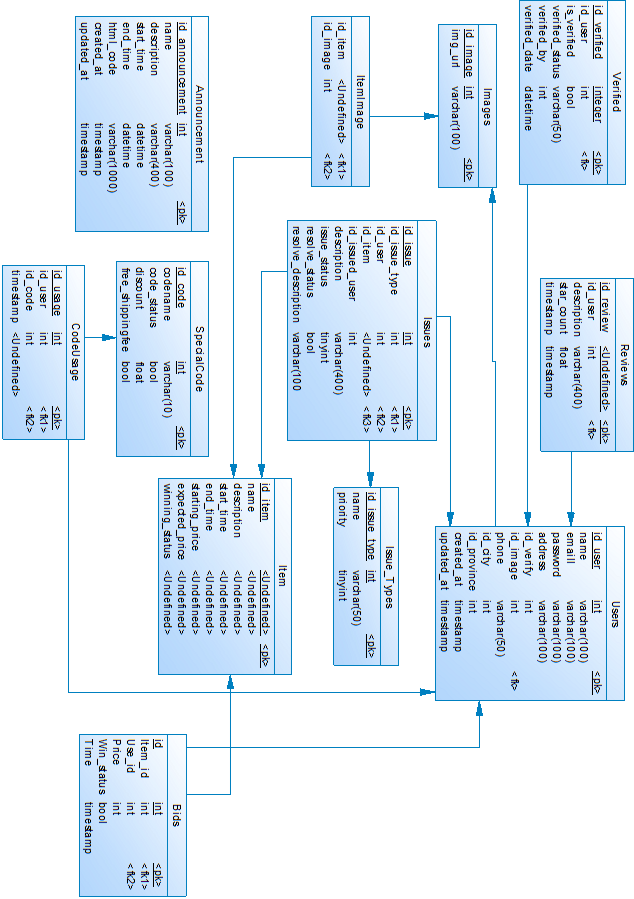
\includegraphics[height=0.6\paperheight]{images/bab3/db/pdm-awal.png}
		\caption{Rancangan Awal PDM untuk Database Relasional}
		\label{pdm-awal}
	\end{figure}
	
	Dan untuk tabel NoSQL dirancang sebagai berikut :
	\begin{figure}[H]
		\centering
		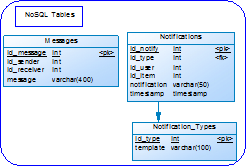
\includegraphics[width=\textwidth]{images/bab3/db/pdm-nosql-awal.png}
		\caption{Rancangan Awal PDM untuk Database Non-Relasional}
		\label{pdm-nosql-awal}
	\end{figure}
	
	Untuk database versi paling \textit{update}, dapat dilihat pada gambar berikut :
	\begin{figure}[H]
		\centering
		
\includegraphics[width=\textwidth]{images/no-image.png}
		\caption{PDM ter\textit{update} untuk Database Relasional}
		\label{pdm-final}
	\end{figure}
	
	Dan untuk tabel NoSQL dirancang sebagai berikut :
	\begin{figure}[H]
		\centering
		
\includegraphics[width=\textwidth]{images/no-image.png}
		\caption{PDM Ter\textit{Update} Database Non-Relasional}
		\label{pdm-nosql-final}
	\end{figure}
	
	Namun, karena pengembangan aplikasi yang bersifat \textit{agile} dan terus berubah karena perkembangan dan \textit{improvization} dari hasil analisa penulis, sifatnya menjadi sangat dinamis.\\

	Berikut akan dipaparkan spesifikasi dan penjelasan setiap tabel.
	\subsubsection{Spesifikasi Tabel User}
	
	\begin{table}[H]
		\centering
		\begin{tabular}{|r|l|l|l|}
			\hline
			\multicolumn{4}{|c|}{\textbf{Tabel items}} \\ \hline
			\textbf{Deskripsi} & \multicolumn{3}{l|}{Tabel ini menyimpan data XX YY ZZ} \\ \hline
			\textbf{Penyimpanan} & \multicolumn{3}{l|}{Transaksional / PostgreSQL} \\ \hline
			\textbf{\begin{tabular}[c]{@{}r@{}}Growth \\ Speed\end{tabular}} & \multicolumn{3}{l|}{\begin{tabular}[c]{@{}l@{}}(masih dipertimbangkan, tapi ini isinya \\ perhitungan/kalkulasi kasar perhitungan \\ penambahan data)\end{tabular}} \\ \hline
			\multicolumn{4}{|c|}{\textbf{Penjelasan Kolom Tabel User}} \\ \hline
			\multicolumn{1}{|l|}{No} & Nama Atribut & Tipe Data & Keterangan \\ \hline
			\begin{tabular}[c]{@{}r@{}}1\\ {[}PK{]}\end{tabular} & ID & INT & \begin{tabular}[c]{@{}l@{}}Autoincrement\\ oleh Sistem\end{tabular} \\ \hline
			2 & Name & varchar(255) & \begin{tabular}[c]{@{}l@{}}Diisi oleh\\ Pengguna\end{tabular} \\ \hline
			\begin{tabular}[c]{@{}r@{}}3\\ {[}FK{]}\end{tabular} & Category\_id & int & Diisi pengguna \\ \hline
			4 & Updated\_at & timestamp & \begin{tabular}[c]{@{}l@{}}Diisi oeh\\ Sistem\end{tabular} \\ \hline
		\end{tabular}
		\caption{Spesifikasi Tabel Z}
		\label{items-tab}
	\end{table}
	
	
		\subsubsection{Spesifikasi Tabel User}
		
		\begin{table}[H]
			\centering
			\begin{tabular}{|r|l|l|l|}
				\hline
				\multicolumn{4}{|c|}{\textbf{Tabel items}} \\ \hline
				\textbf{Deskripsi} & \multicolumn{3}{l|}{Tabel ini menyimpan data XX YY ZZ} \\ \hline
				\textbf{Penyimpanan} & \multicolumn{3}{l|}{Transaksional / PostgreSQL} \\ \hline
				\textbf{\begin{tabular}[c]{@{}r@{}}Growth \\ Speed\end{tabular}} & \multicolumn{3}{l|}{\begin{tabular}[c]{@{}l@{}}(masih dipertimbangkan, tapi ini isinya \\ perhitungan/kalkulasi kasar perhitungan \\ penambahan data)\end{tabular}} \\ \hline
				\multicolumn{4}{|c|}{\textbf{Penjelasan Kolom Tabel User}} \\ \hline
				\multicolumn{1}{|l|}{No} & Nama Atribut & Tipe Data & Keterangan \\ \hline
				\begin{tabular}[c]{@{}r@{}}1\\ {[}PK{]}\end{tabular} & ID & INT & \begin{tabular}[c]{@{}l@{}}Autoincrement\\ oleh Sistem\end{tabular} \\ \hline
				2 & Name & varchar(255) & \begin{tabular}[c]{@{}l@{}}Diisi oleh\\ Pengguna\end{tabular} \\ \hline
				\begin{tabular}[c]{@{}r@{}}3\\ {[}FK{]}\end{tabular} & Category\_id & int & Diisi pengguna \\ \hline
				4 & Updated\_at & timestamp & \begin{tabular}[c]{@	{}l@{}}Diisi oeh\\ Sistem\end{tabular} \\ \hline
			\end{tabular}
			\caption{Spesifikasi Tabel Z}
			\label{items-2tab}
		\end{table}
	
  
  \subsection{Perancangan Arsitektur Aplikasi}
	
      \begin{figure}[H]
        \centering
        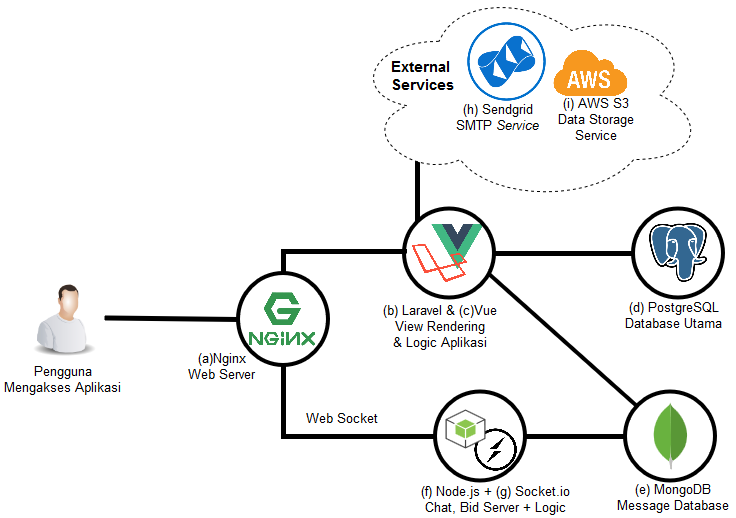
\includegraphics[width=\textwidth]{images/bab3/diagram/arsitektur-awal.png}
        \caption{Arsitektur Aplikasi Lelang Online 
        		\\
                \textit{External Services} artinya adalah menggunakan \textit{service} dari luar, tidak dibangun sendiri. }
        \label{arsitektur-app-final}
      \end{figure}
    
    \subsubsection{\textbf{\textsc{Nginx} sebagai WebServer dan Proxy Server}}
    {\scshape Nginx} adalah web server multifungsi - dimana selain berfungsi sebagai Webserver, namun juga bisa berfungsi sebagai Load Balancer. Dalam awal pembuatan aplikasi, \textsc{Nginx} hanya digunakan sebagai \textit{web server} untuk melayani permintaan halaman Web dari pengguna.
    \\
    Namun, saat \textit{deployment}, banyak sekali terjadi \textit{issue} yang berkaitan dengan \textit{ssl certificate}, sehingga pada akhirnya Nginx juga digunakan sebagai \textit{proxy server} - dimana Nginx mempunyai fungsi baru yaitu \textit{redirecting request=request} yang masuk ke dalam server, dan meneruskannya ke proses dalam server yang bertugas memproses \textit{request} tersebut.
	   \\
    Beberapa masalah yang ditemukan penulis, jika tidak menggunakan fitur \textsc{Nginx} sebagai proxy server untuk aplikasi Soket yang berbeda port adalah sebagai berikut :
	    \begin{itemize}[noitemsep,topsep=0pt]
	    \item CORS (Cross Origin Reference Source)
	    \newline
	    Dimana pada saat browser mengakses soket dari port lain (meskipun domainnnya sama), browser menganggap bahwa sambungan dari port lain tersebut sebagai \textit{security threat} dan otomatis memutuskan sambungan.
	    \item ERROR :: INSECURE RESPONSE!
	    \newline
	    Hal ini terjadi saat browser membuka sebuah web dengan https - namun mengakses koneksi soket yang tidak terproteksi dengan https. Hal ini juga membuat browser menganggap ini sebagai \textit{security threat}, dan tidak membuka \textit{reply} dari koneksi soket yang tidak terproteksi dengan https tersebut.
	    \end{itemize}
    
    \subsubsection {\textbf{Laravel dan Logika Aplikasi}}
    \textsc{Laravel}, bertugas sebagai Bos Besar, pengelola data dan manajemen data, dan pelayan \textit{request} dalam aplikasi Lelang online ini. Semua request diteruskan, dan diproses oleh \textsc{Laravel}, dan diproses oleh Laravel. 	    
    
    \subsubsection{\textbf{Vue.js sebagai \textit{View Renderer} }}
	Penggunaan Vue.js yang digunakan oleh penulis dimaksudkan untuk membagi beban kerja/\textit{workloads} antara Server dan Pengguna. \\
    Seperti yang saya paparkan pada subbab Analisa (poin \ref{alasan-ux-ecommerce-indonesia} dan \ref{alasan-app-serupa}), ini ditujukan sebagai solusi cerdas untuk mengakali \textit{delay querying} yaitu \textit{sharing workloads} antara server dan client(browser) dan juga \textit{user experience behaviour}, agar lebih sabar menunggu waktu \textit{loading} aplikasi). \\
    Namun, untuk optimasinya, mengingat laju pertambahan data gambar maupun barang pada aplikasi \textit{e-commerce} pastiya sangat cepat dan masif, maka penulis membagi \textit{workloads} antara Laravel sebagai \textit{web server}, dan browser pengguna - dengan menggunakan Vue.js.
    
    
    \subsubsection{\textbf{PostgreSQL sebagai DBMS Transaksional}}
    PostgreSQL bertugas menyimpan data-data yang bersifat transaksional, seperti data \textit{master} : data pengguna, data barang yang terdaftar, data riwayat lelang, data \textit{rating} dan \textit{review}, dan lain-lain.
    
    \subsubsection{\textbf{MongoDB} sebagai DBMS Non-Transaksional - NOSQL}
    MongoDB akan digunakan untuk menyimpan :
	    \begin{itemize}[noitemsep,topsep=0pt]
	    \item Daftar pesan/\textit{chat} yang dikirimkan pengguna
	    \item Daftar \textit{conversation} untuk mempermudah menampilkan \textit{inbox} pengguna
	    \item Daftar gambar/foto yang diunggah bersama dengan barang yang diupload.
	    \end{itemize}
	Ekspektasi dalam menggunakan database NoSQL adalah agar proses \textit{query} lebih cepat, tidak memberatkan database transaksional.

	\subsubsection{\textbf{Node.js} sebagai Asynchronous-Request Server}
    Server yang dibangun dengan menggunakan Node.js akan mengakomodasi \textit{request} yang bersifat \textit{event-driven} dan bersifat asinkronus, seperti transaksi lelang/\textit{bidding} dan \textit{chatting}.
    
    \subsubsection{\textbf{SendGrid} sebagai SMTP Service}
    Untuk mengakomodasi fitur verifikasi otomatis lewat email, dibutuhkan sebuah SMTP service untuk mengirimkan email dari aplikasi ke alamat email pengguna. Dalam hal ini, yang digunakan adalah SendGrid Service.
    
    \subsubsection{\textbf{Amazon S3} sebagai Data Storage Service}
    Untuk menyimpan gambar-gambar dari barang yang di\textit{upload} pada saat mendaftarkan barang.

	\subsubsection{\textbf{Laravel Dusk}}
	Untuk ini, akan dibahas lebih lanjut pada bagian pengujian, karena ini adalah bagian dari perangkat lunak yang digunakan sebagai \textit{testing} dalam arsitektur tersebut.
      
   
      
    
  
  \subsection{Perancangan Alur Data}


  
  \subsection{Kamus Data}
  
  
    w\chapter{IMPLEMENTASI}
  Pada bab ini dibahas mengenai implementasi aplikasi sesuai dengan perancangan sistem yang telah dijelaskan sebelumnya. Bahasa pemrograman yang digunakan antara lain PHP, SQL, Javascript.
  
  \section{Lingkungan Implementasi}
  Lingkungan pembangunan dijelaskan pada subbab ini.
  \subsection{Lingkungan Pembangun Perangkat Keras}
  Perangkat keras yang digunakan dalam pembuatan tugas akhir ini adalah sebagai berikut :
  \begin{enumerate}
  \item Personal Komputer
  		\begin{enumerate}
  		\item Prosesor XX
        \item Memori YY
        \item Sistem Operasi ZZ
  		\end{enumerate}
  \item VPS
  	VPS yang digunakan dalam lingkungan pembangunan di\textit{host} oleh DigitalOcean dengan spesifikasi sebagai berikut :
  		\begin{enumerate}
  		\item Prosesor XX
        \item Memori YY
        \item Sistem Operasi ZZ
  		\end{enumerate}
  \end{enumerate}
  
  \subsection{Lingkungan Pembangun Perangkat Lunak}
  Spesifikasi perangkat lunak yang digunakan untuk membuat tugas akhir ini adalah sebagai berikut:
  \begin{enumerate}
  \item Web Browser Google Chrome
  \item PgAdmin
  \item PHPStorm sebagai IDE PHP
  \item Nano untuk \textit{shell text editor}
  \item Postman
  \item Power Designer
  \end{enumerate}
  
\section{Implementasi Antarmuka}
	
    \subsection{Antarmuka Halaman A}
    Penjelasan otorisasi terhadap antarmuka A, link yang tersedia dalam antarmuka A, dan penjelasan \textit{exception} jika terjadi masalah baik otorisasi ataupun autentikasi saat mengakses antarmuka ini.
  
      \begin{figure}[H]
        \centering
        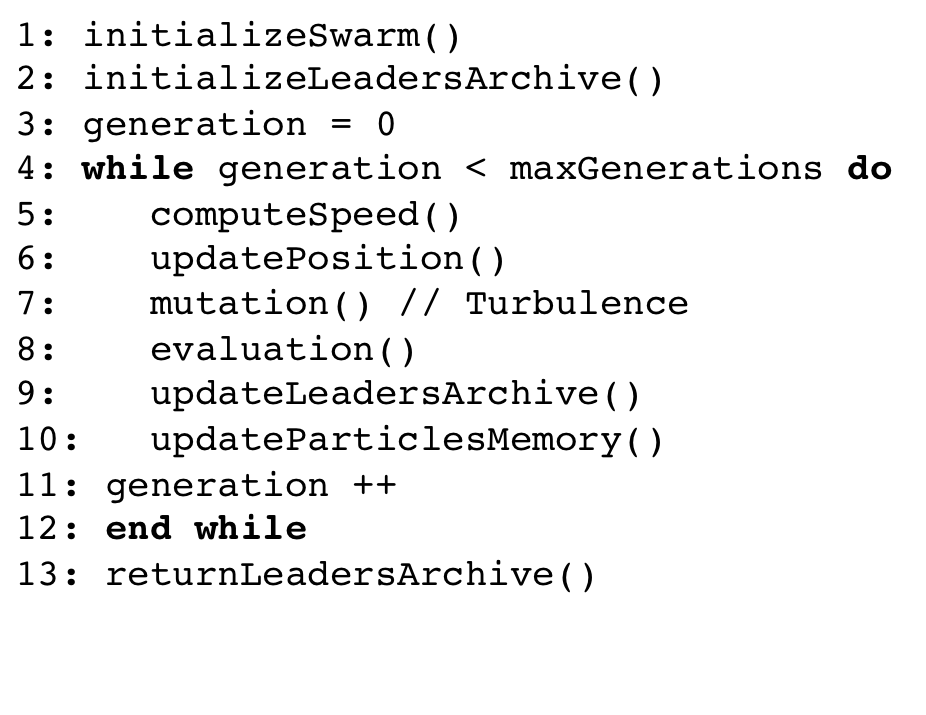
\includegraphics[width=\linewidth]{images/bab4/smpso_code.png}
        \caption{ Pseudocode Controller untuk Menampilkan Antarmuka A }
        \label{pdm}
      \end{figure}
      
    \subsection{Antarmuka Halaman B}
    Penjelasan otorisasi terhadap antarmuka B, link yang tersedia dalam antarmuka B, dan penjelasan \textit{exception} jika terjadi masalah baik otorisasi ataupun autentikasi saat mengakses antarmuka ini.
  
      \begin{figure}[H]
        \centering
        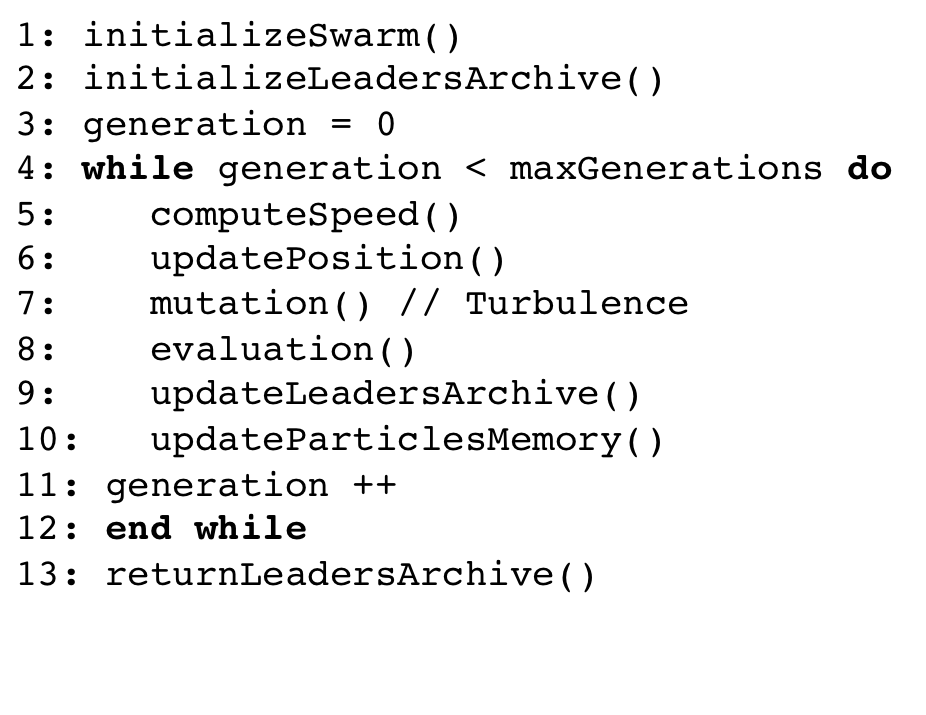
\includegraphics[width=\linewidth]{images/bab4/smpso_code.png}
        \caption{ Pseudocode Controller untuk Menampilkan Antarmuka B }
        \label{pdm}
      \end{figure}
    
    
\section{Pemasangan Proyek}
	Pembangunan dilakukan secara online, dan tersebar (tidak hanya menggunakan satu \textit{service provider} saja.
    Berikut dijelaskan langkah-langkah pembangunan proyek:
    
    \subsection{Konfigurasi Domain}
    Domain yang dipilih berasal dari Namecheap.com , dengan langkah-langkah konfigurasi sebagai berikut :
    \begin{enumerate}
    \item Langkah 1
    \item Langkah 2
    \end{enumerate}
    \subsection{Konfigurasi VPS}
    Domain yang dipilih berasal dari DigitalOcean dan Google Cloud Computing , dengan langkah-langkah konfigurasi sebagai berikut :
    \begin{enumerate}
    \item DigitalOcean
      \begin{enumerate}
      \item Langkah 1
      \item Langkah 2
      \end{enumerate}
    \item Google Cloud Computing
      \begin{enumerate}
      \item Langkah 1
      \item Langkah 2
      \end{enumerate}
    \end{enumerate}
    
    \subsection{Konfigurasi PostgreSQL}
    PostgreSQL diinstal dalam VPS, dengan langkah-langkah konfigurasi sebagai berikut :
    \begin{enumerate}
    \item Langkah 1
    \item Langkah 2
    \end{enumerate}
    
    \subsection{Konfigurasi Node.js}
    Node.js diinstall dalam VPS, dengan langkah-langkah konfigurasi sebagai berikut :
    \begin{enumerate}
    \item Langkah 1
    \item Langkah 2
    \end{enumerate}
    
    \subsection{Konfigurasi MongoDB}
    MongoDB diinstall dalam VPS, dengan langkah-langkah konfigurasi sebagai berikut :
    \begin{enumerate}
    \item Langkah 1
    \item Langkah 2
    \end{enumerate}
    
    \subsection{Konfigurasi SMTP Service}
    SMTP \textit{service} yang digunakan berasal dari sendgrid.net, dengan langkah-langkah konfigurasi sebagai berikut :
    \begin{enumerate}
    \item Langkah 1
    \item Langkah 2
    \end{enumerate}

    	\chapter{PENGUJIAN DAN EVALUASI}

	Pada bab ini akan dibahas mengenai pengujian dan evaluasi pada aplikasi. Pengujian yang dilakukan terdiri dari dua pengujian yaitu pengujian fungsionalitas sistem dan pengujian statistik. Pengujian fungsionalitas mengacu pada daftar fungsionalitas pada bab III (Desain dan Perancangan) Sedangkan pengujian statistik dilakukan untuk membuktikan bahwa aplikasi benar telah mencapai tujuan yang dipaparkan pada Bab II poin 2.
    
      
    \section{Pengujian}
	Aplikasi yang telah dibangun dapat dikatakan berhasil jika sudah memenuhi kebutuhan fungsional dan nonfungsional yang telah didefinisikan pada Tabel \ref{tabel-fungsional} dan \ref{tabel-non-fung}. Pada bab ini akan dibahas mengenai pengujian dan evaluasi pada aplikasi yang dikembangkan. Pengujian yang dilakukan terdiri dari dua pengujian yaitu pengujian fungsionalitas sistem dan pengujian statistik. Pengujian fungsionalitas mengacu pada kebutuhan fungsionalitas yang didefinisikan pada Tabel \ref{tabel-fungsional}. Sedangkan pengujian statistik dilakukan untuk menguji apakah aplikasi telah memenuhi kebutuhan nonfungsional yang telah didefinisikan pada Tabel \ref{tabel-non-fung}.

	
	\subsection{Metode Pengujian}
		
	Metode pengujian dirancang sesuai dengan kebutuhan fungsional dan nonfungsional yang telah didefinisikan. Metode-metode pengujian yang digunakan pada tugas akhir ini adalah sebagai berikut:
	
	\begin{enumerate}
	\item \textbf{Pengujian Fungsionalitas} \\
	Pengujian fungsionalitas sistem dilakukan secara mandiri dengan menyiapkan sejumlah skenario. Deskripsi proses pengujian secara lengkap akan dijelaskan pada subbab \ref{uji-fungsional}.
	
	\item \textbf{Pengujian Performa}\\
	Pengujian performa dilakukan pada setiap kasus penggunaan, dan mencatat waktu yang dibutuhkan untuk menampilkan sebuah halaman dan atau melakukan sebuah \textit{request} ke aplikasi. Deskripsi proses pengujian performa akan secara lengkap dijelaskan pada subbab \ref{uji-performa}.
	
	\item \textbf{Pengujian \textit{User Experience}} \\
	Pengujian \textit{user experience} dilakukan secara statistik, untuk menguji apakah bahwa benar aplikasi yang dibangun memberikan \textit{positive user experience} kepada penggunanya. \textit{Key performance indicator} yang digunakan didasarkan pada paper ``Development of an Instrument Measuring User Satisfaction of the Human-Computer Interface''. Deskripsi proses pengujian performa akan secara lengkap dijelaskan pada subbab \ref{uji-ux}.
	
	\item \textbf{Pengujian \textit{Maintainability}} \\
	Pengujian \textit{maintainability} dimaksudkan untuk menguji apakah benar aplikasi yang dibangun bersifat \textit{maintainable} kepada \textit{developer}. Pengujian ini dilakukan secara statistik, dengan mengacu kepada paper ``A Software Maintainability Evaluation Methodology''. Deskripsi proses pengujian secara lengkap akan dijelaskan pada subbab \ref{uji-maintainability}.
	\end{enumerate}

		
	\subsection{Pengujian Fungsionalitas}
	\label{uji-fungsional}
			
	\subsubsection{Pengujian Fungsionalitas Manajemen Autentikasi}	
	\input{Chapters\Details\bab5\fungsionalitas\1-autentikasi}
%	\input{Chapters\Details\bab5\fungsionalitas\main}
		
	\subsubsection{Pengujian Fungsionalitas Manajemen Penawaran}
	\input{Chapters\Details\bab5\fungsionalitas\2-penawaran}
		
	\subsubsection{Pengujian Fungsionalitas Manajemen Barang Lelang}
	\input{Chapters\Details\bab5\fungsionalitas\3-barang}
			
	\subsubsection{Pengujian Fungsionalitas Manajemen Interaksi Antarpengguna}
	\input{Chapters\Details\bab5\fungsionalitas\4-interaksi}
	
	\subsubsection{Pengujian Fungsionalitas Manajemen Laporan}
	\input{Chapters\Details\bab5\fungsionalitas\5-laporan}
	
	\subsubsection{Pengujian Fungsionalitas Manajemen Kupon}
	\input{Chapters\Details\bab5\fungsionalitas\6-kupon}
	
			

	
	
	\subsection{Pengujian Kecepatan}
	\label{uji-performa}
	
	\subsubsection{Proses Pengujian}
	\input{Chapters\Details\bab5\fungsionalitas\process}
	
	\subsubsection{Hasil Pengujian}
	\input{Chapters\Details\bab5\fungsionalitas\hasil}
	
	\subsection{User Experience Assesment}
	\label{[uji-ux}
		
	\subsubsection{Deskripsi Pengujian}
	\input{Chapters/Details/bab5/ux/proses}
	
	\subsubsection{Hasil Pengujian}
	\input{Chapters/Details/bab5/ux/hasil}
	
	\subsection{Maintainability Assesment}
	\label{uji-maintainability}
		
	\subsubsection{Proses Pengujian}
	\input{Chapters\Details\bab5\maintainability\proses}
	
	\subsubsection{Hasil Pengujian}
	\input{Chapters\Details\bab5\fungsionalitas\hasil}
	
	
		
		

    
    \section{Evaluasi}
	Pada subbab ini, penulis akan memaparkan hasil analisa terhadap aplikasi, perspektif non-IT terhadap pengerjaan maupun lingkup pekerjaan dari aplikasi Lelang Online ini.
	
	\subsection{Evaluasi Regulasi}
	
	
	\subsection{Evaluasi Market}
	

	\subsection{Summary}
    

    %\section{Struktur Dokumen \LaTeX{}}
Dokumen \LaTeX{} terdiri dari struktur yang dibuat berdasarkan struktur dokumen sehari-hari. Sebagai penulis dokumen, Anda wajib menggunakan struktur ini sehingga \LaTeX{} dapat melakukan hal lain yang membantu Anda dalam mengorganisir dokumen seperti misalnya pembuatan Daftar Isi. Berikut adalah struktur dokumen yang ada di \LaTeX{} diurutkan berdasarkan hirarkinya.

\begin{ltabulary}{|L|L|} % L = Rata kiri untuk setiap kolom, | = garis batas vertikal.

% Kepala tabel, berulang di setiap halaman
\caption{Struktur hirarki dokumen \LaTeX{}} \label{tabelStrukturDokumen} \\
\hline
\textbf{Nama} & \textbf{Peruntukkan} \\ \hline

\endhead
\endfoot
\endlastfoot

% Isi Tabel
\textbf{\textbackslash{}part\{Judul Bagian\}} & \texttt{book} \\ \hline
\textbf{\textbackslash{}chapter\{Judul Bab\}} & \texttt{book} dan \texttt{report} \\ \hline
\textbf{\textbackslash{}section\{Judul Subbab\}} & semua kecuali \texttt{letter} \\ \hline
\textbf{\textbackslash{}subsection\{Judul Subsubbab\}} & semua kecuali \texttt{letter} \\ \hline
\textbf{\textbackslash{}subsubsection\{Judul Subsubsubbab\}} & semua kecuali \texttt{letter} \\ \hline
\textbf{\textbackslash{}paragraph\{Judul Paragraf\}} & semua\\ \hline

\end{ltabulary}

\subsection{Pengujian Performa}
      Pengujian 
      \subsubsection{Pengujian Kecepatan Fitur A}
      Pengujian fitur ini dilakukan pada lingkungan uji \ref{env_uji1}, dan untuk lebih lengkapnya dapat dilihat pada tabel \ref{uji1}
      \begin{table}[]
      \centering
      \caption{Pengujian Fitur B}
      \label{uji2}
      \begin{tabular}{llll}
      \multicolumn{1}{c}{\textbf{ID}} & \multicolumn{3}{c}{\textbf{TA-UJI.Proses}}        \\
      Referensi Proses Penggunaan     & \multicolumn{3}{l}{}                              \\
      Nama                            & \multicolumn{3}{l}{}                              \\
      Tujuan Pengujian                & \multicolumn{3}{l}{\multirow{2}{*}{}}             \\
      \textbf{Skenario Pengujian}     & \multicolumn{3}{l}{}                              \\
      Langkah Pengujian               & \multicolumn{3}{l}{}                              \\
      Kecepatan Buka Halaman          & Halaman       & \multicolumn{2}{l}{Google Chrome} \\
                                      & A             & 18 KB           & 0.987s         
      \end{tabular}
      \end{table}
      
    \chapter{PENUTUP}
  Bab ini membahas kesimpulan yang dapat diambil dari tujuan pembuatan sistem dan hubungannya dengan hasil uji coba dan evaluasi yang telah dilakukan. Selain itu, terdapat beberapa saran yang bisa dijadikan acuan untuk melakukan pengembangan dan penelitian lebih lanjut.
  \section{Kesimpulan}
  Dari proses perancangan, implementasi dan pengujian terhadap sistem, dapat diambil beberapa kesimpulan berikut:
  \begin{enumerate}
    \item Kualitas perancangan dan desain sistem dan fleksibilitas sistem sangat penting dalam rancang bangun aplikasi jual-beli online, karena sifat perubahan yang sangat cepat.
    \item \textit{User Experience} adalah faktor yang sangat penting dalam kesuksesan platform jual-beli online
    \item Selain \textit{user experience}, \textit{maintainability} juga sangat penting karena yang menjaga dan memperbarui perangkat lunak jika ada perubahan adalah \textit{developer} sendiri. Jika sebuah sistem \textit{maintainability}nya buruk, maka sistem tersebut juga tidak fleksibel terhadap perubahan karena \textit{developer} juga pasti pusing untuk menambahkan fitur yang 
  \end{enumerate}
  
  \section{Saran}
  Berikut beberapa saran yang diberikan untuk pengembangan lebih lanjut:
  \begin{enumerate}
    \item Mengikutsertakan pihak yang \textit{capable}/kredibel dan ahli di bidang hukum dan \textit{bussiness process} untuk menetapkan alur, memperbaiki alur dan membuat alur monitoring untuk proses lelang yang lebih aman, kredibel.
    \item Mempelajari platform lelang \textit{online} di luar negeri yang sudah sukses, yakni mempelajari ide-ide, alur aktivitas dan penggunaan kaidah \textit{user experience} dan \textit{usability} dalam website tersebut dan dampaknya terhadap \textit{revenue}.
  \end{enumerate}
  


    % Daftar Pustaka
    \bibliography{Zotero}
    \bibliographystyle{ieeetr}
    
    \appendix % Halaman lampiran, dengan judul LAMPIRAN X
    
\chapter{Kode Sumber}
\chapter{Kuisioner Pengguna}
\begin{figure}[H]
	\centering
	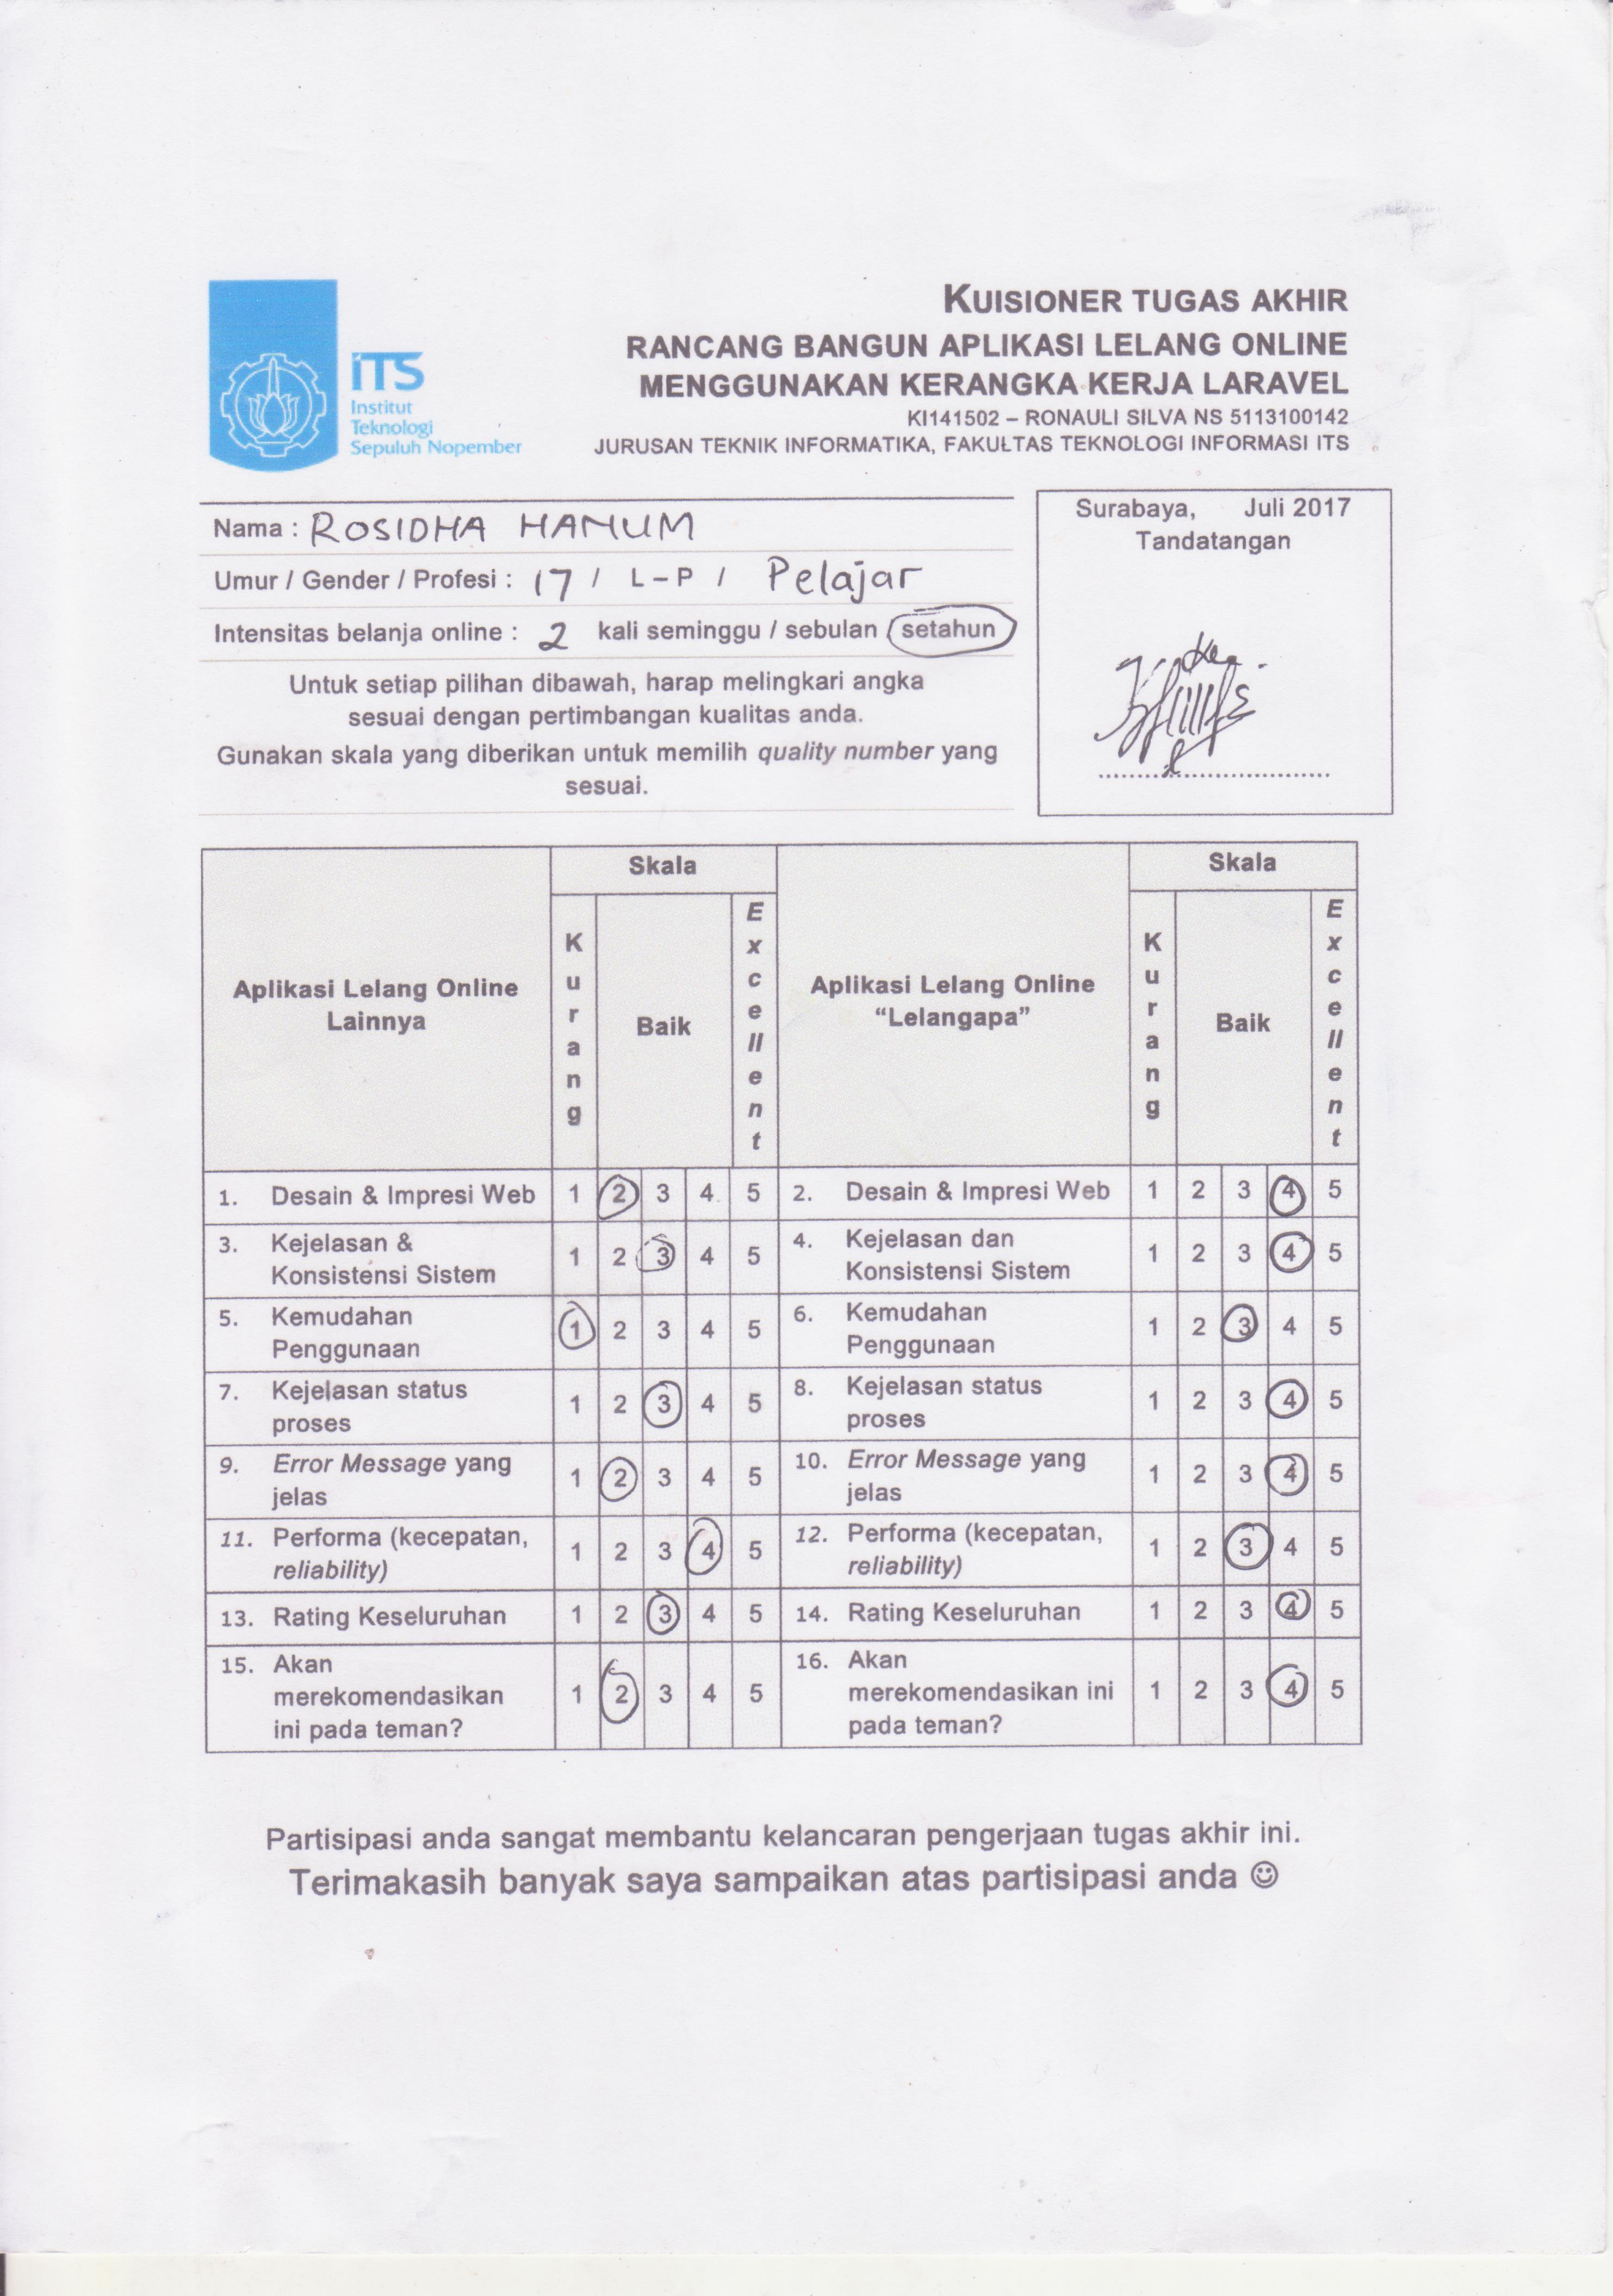
\includegraphics[width=\textwidth]{images/bab5/ujipengguna/1.jpg}
	\caption{Kuisioner Pengguna 1}
	\label{quest-1}
\end{figure}
\begin{figure}[H]
	\centering
	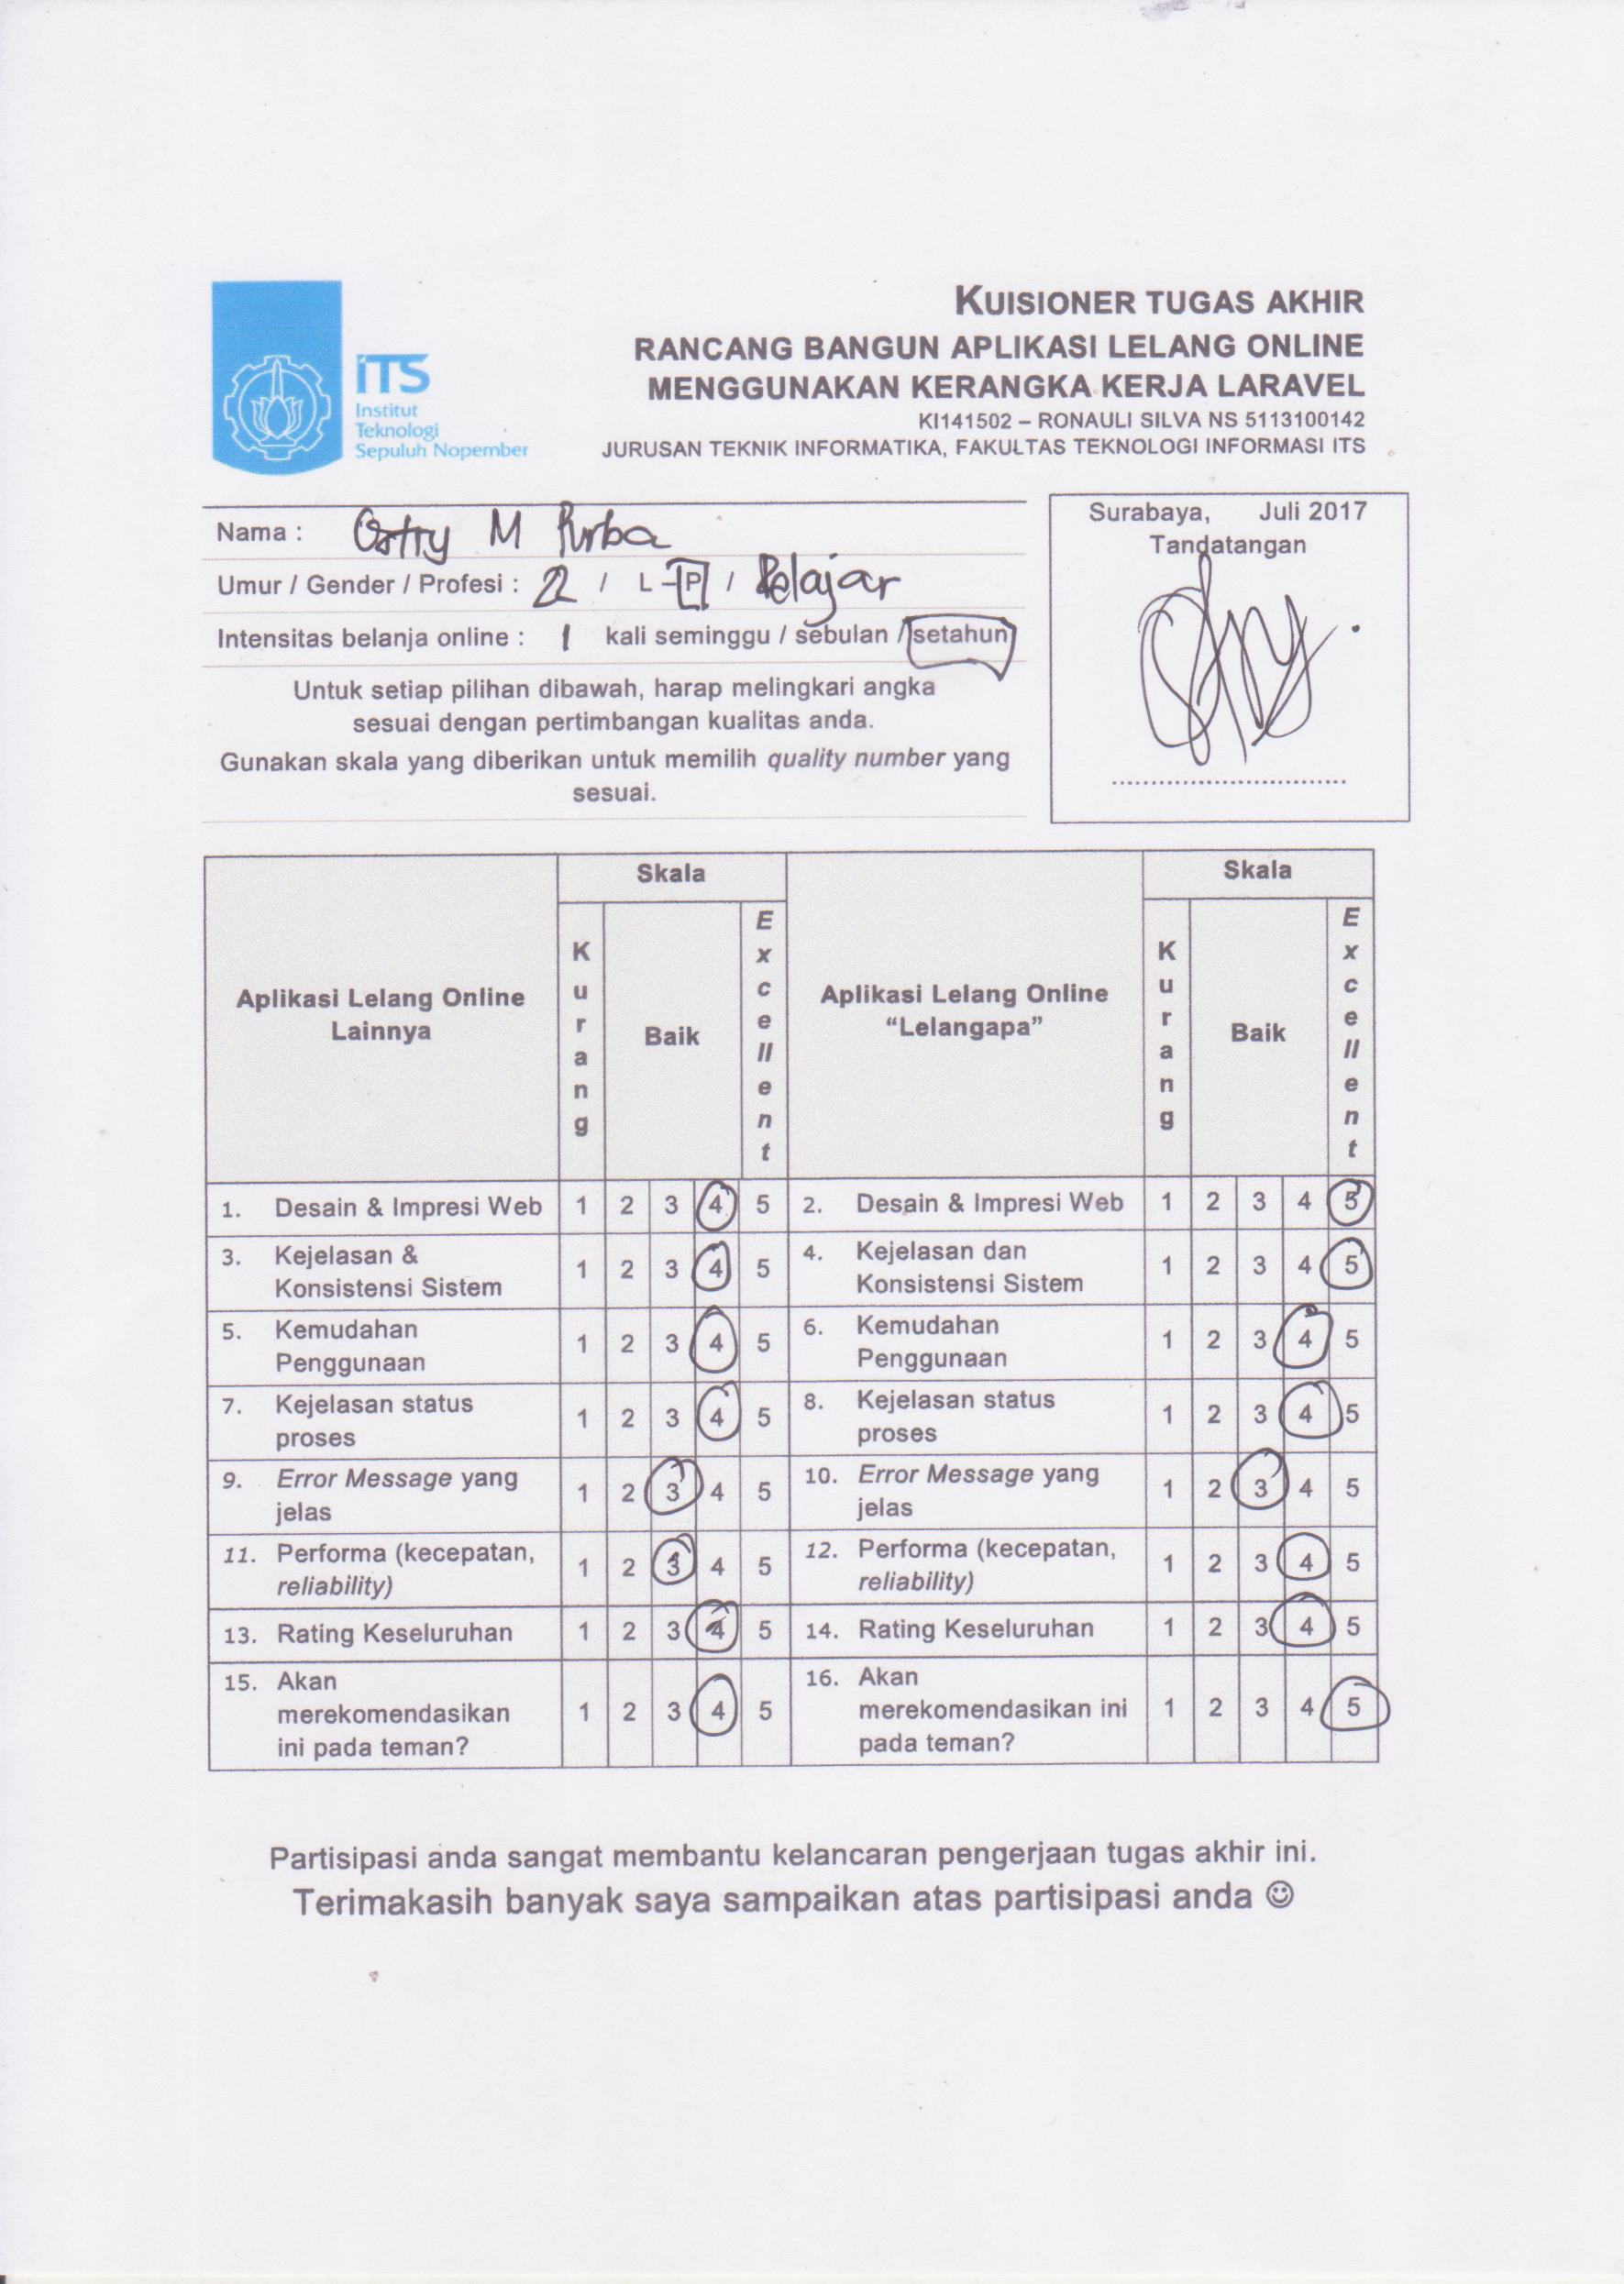
\includegraphics[width=\textwidth]{images/bab5/ujipengguna/2.jpg}
	\caption{Kuisioner Pengguna 2}
	\label{quest-2}
\end{figure}
\begin{figure}[H]
	\centering
	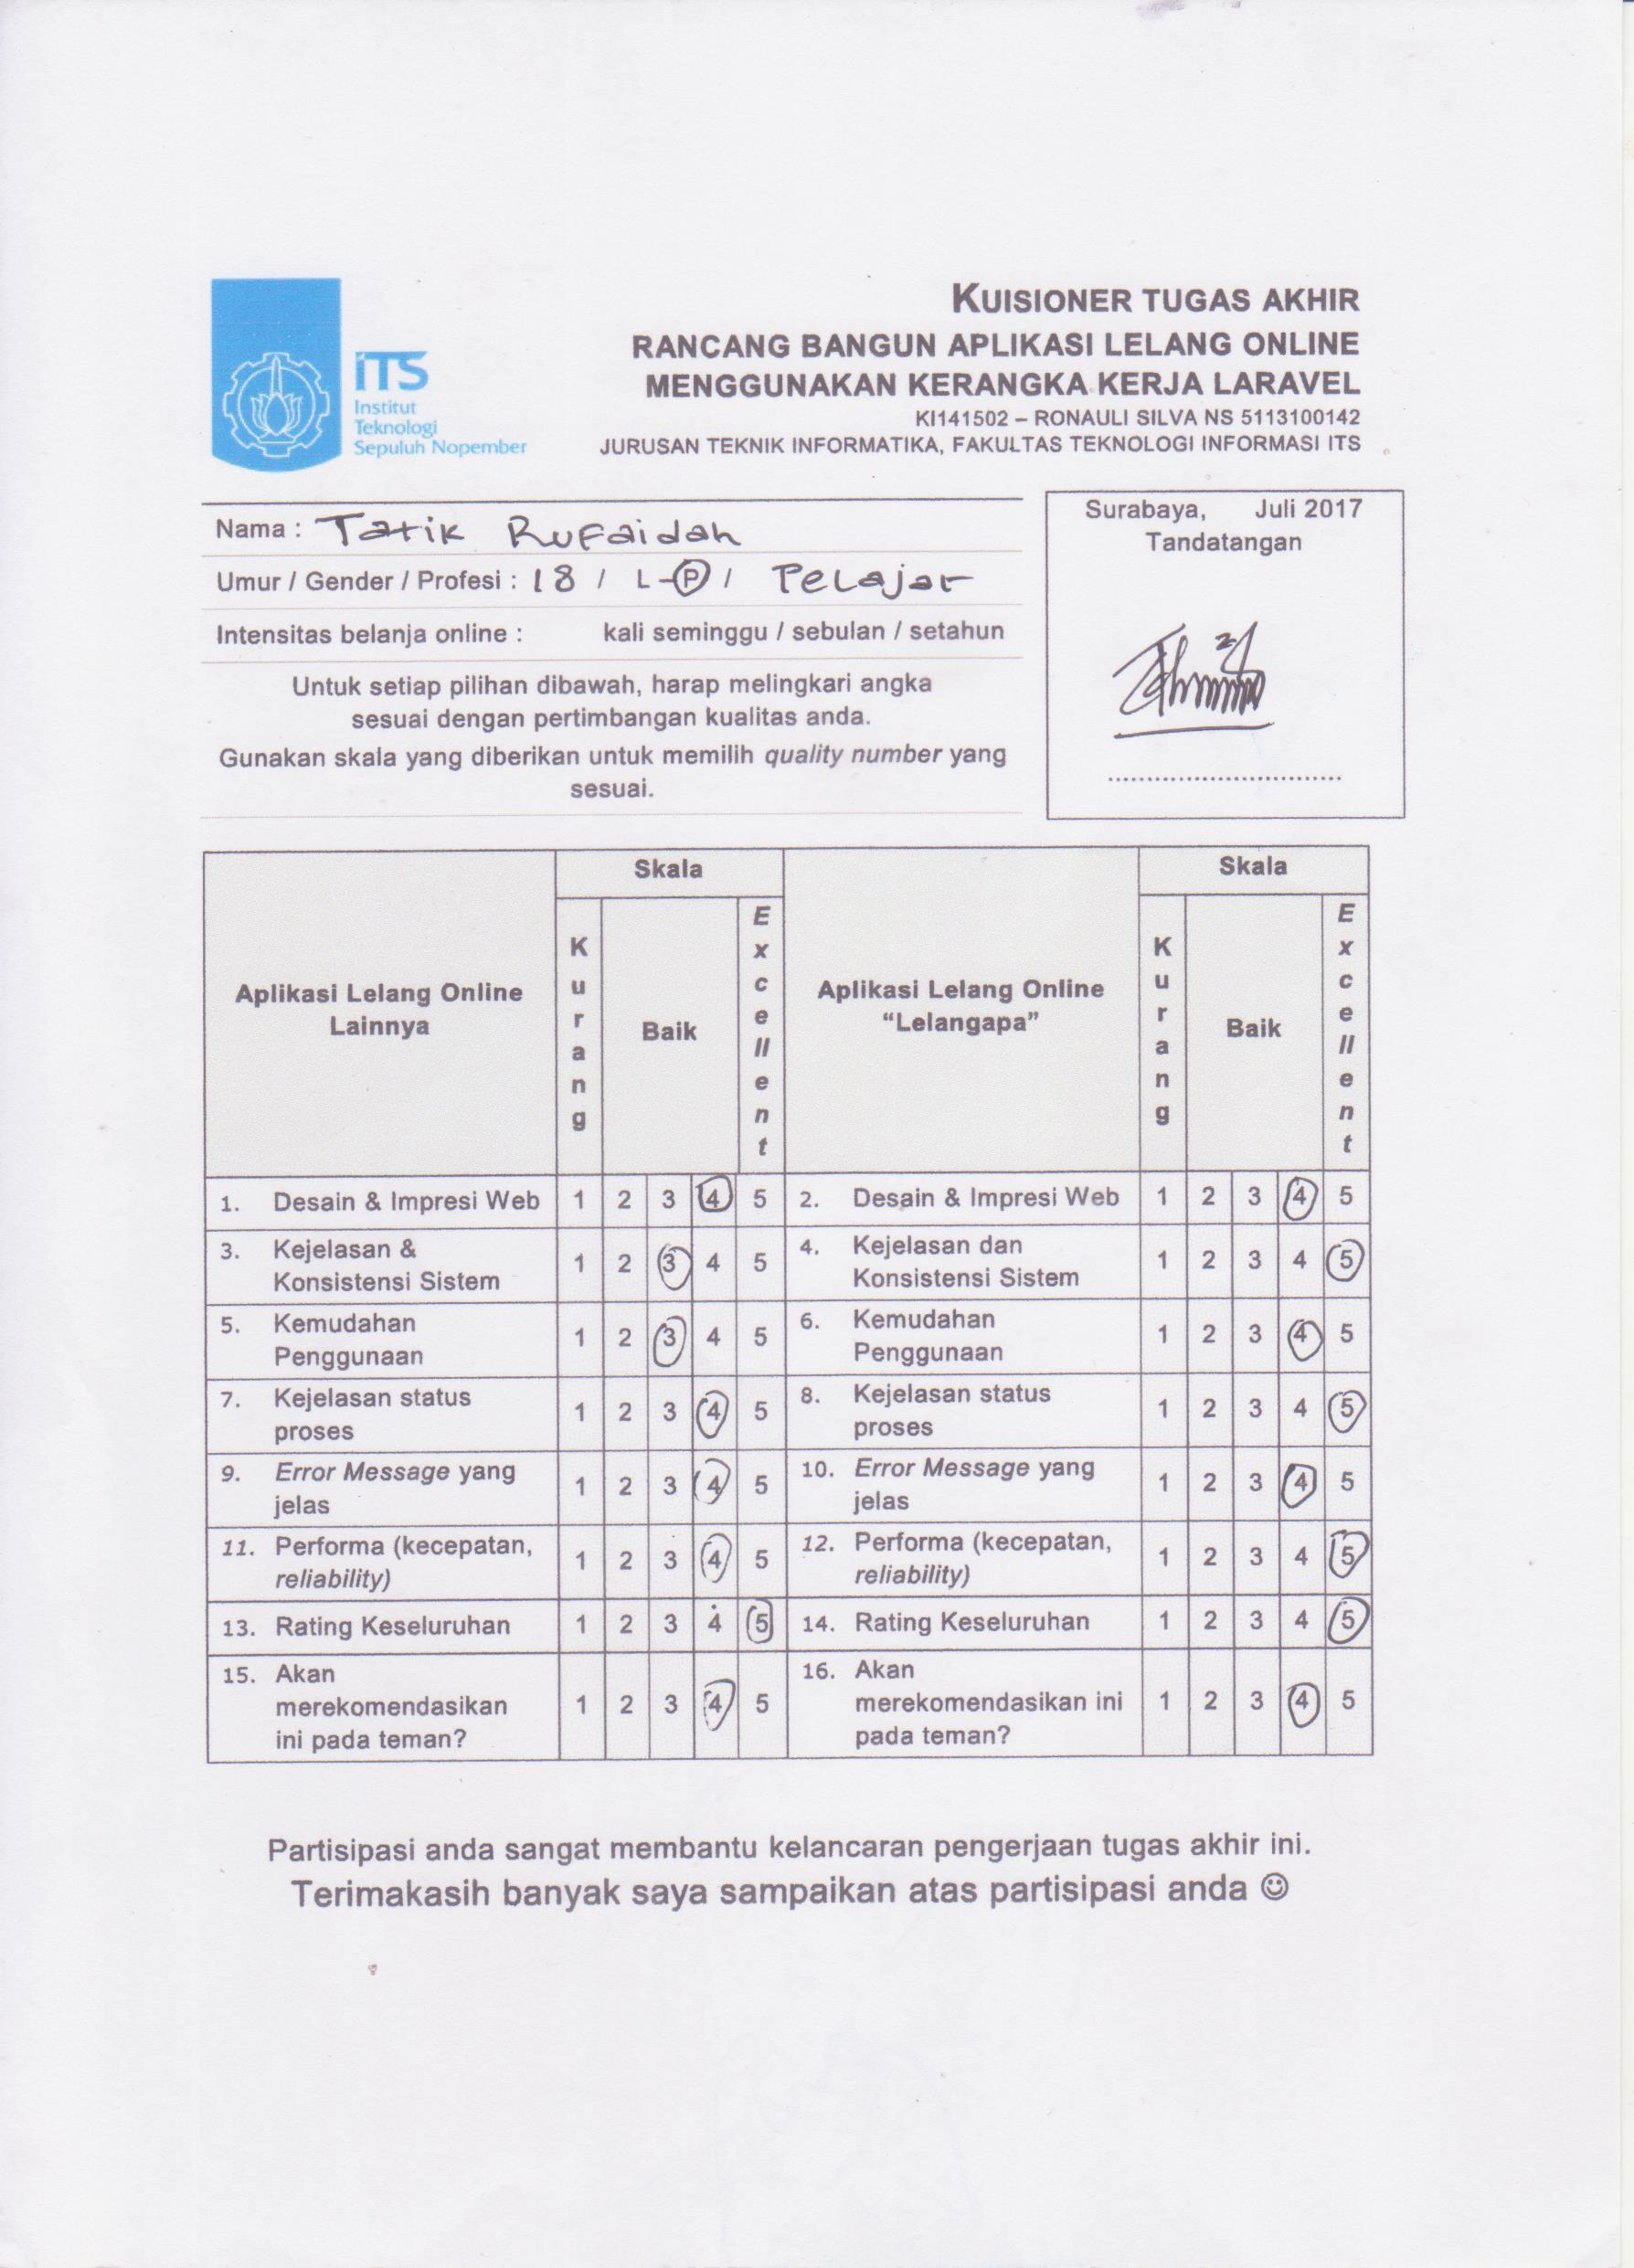
\includegraphics[width=\textwidth]{images/bab5/ujipengguna/3.jpg}
	\caption{Kuisioner Pengguna 3}
	\label{quest-3}
\end{figure}
\begin{figure}[H]
	\centering
	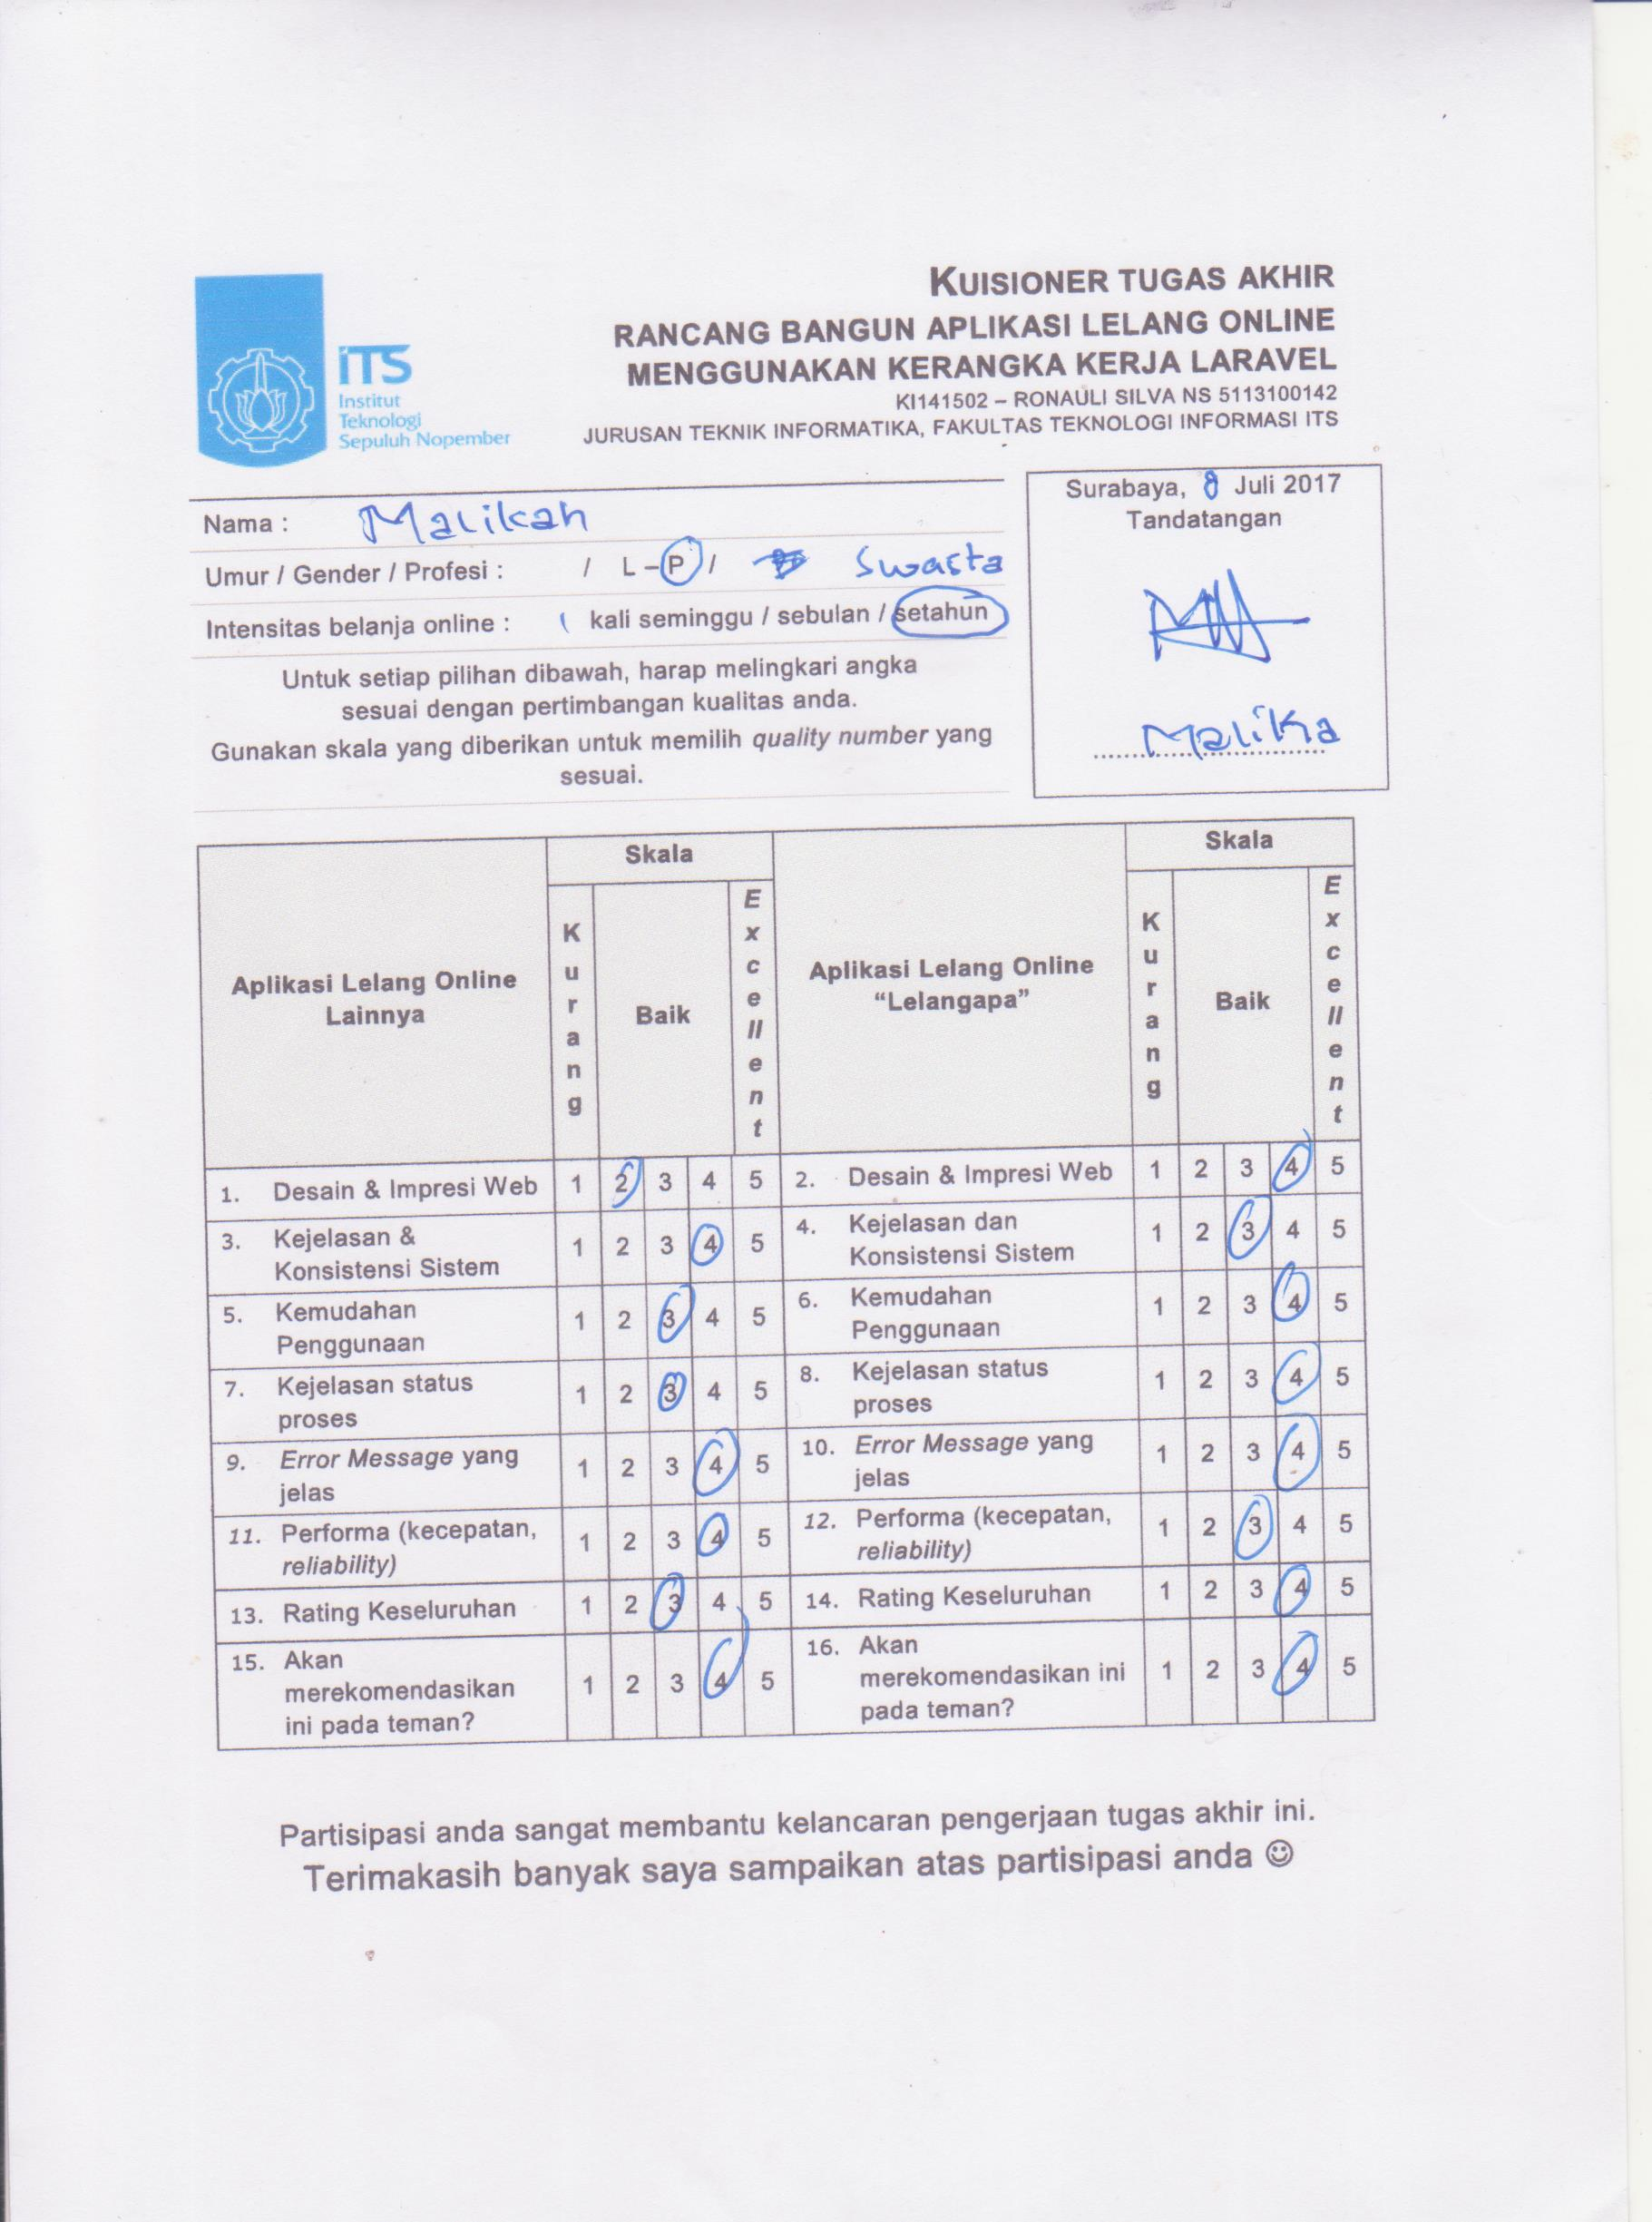
\includegraphics[width=\textwidth]{images/bab5/ujipengguna/4.jpg}
	\caption{Kuisioner Pengguna 4}
	\label{quest-4}
\end{figure}
\begin{figure}[H]
	\centering
	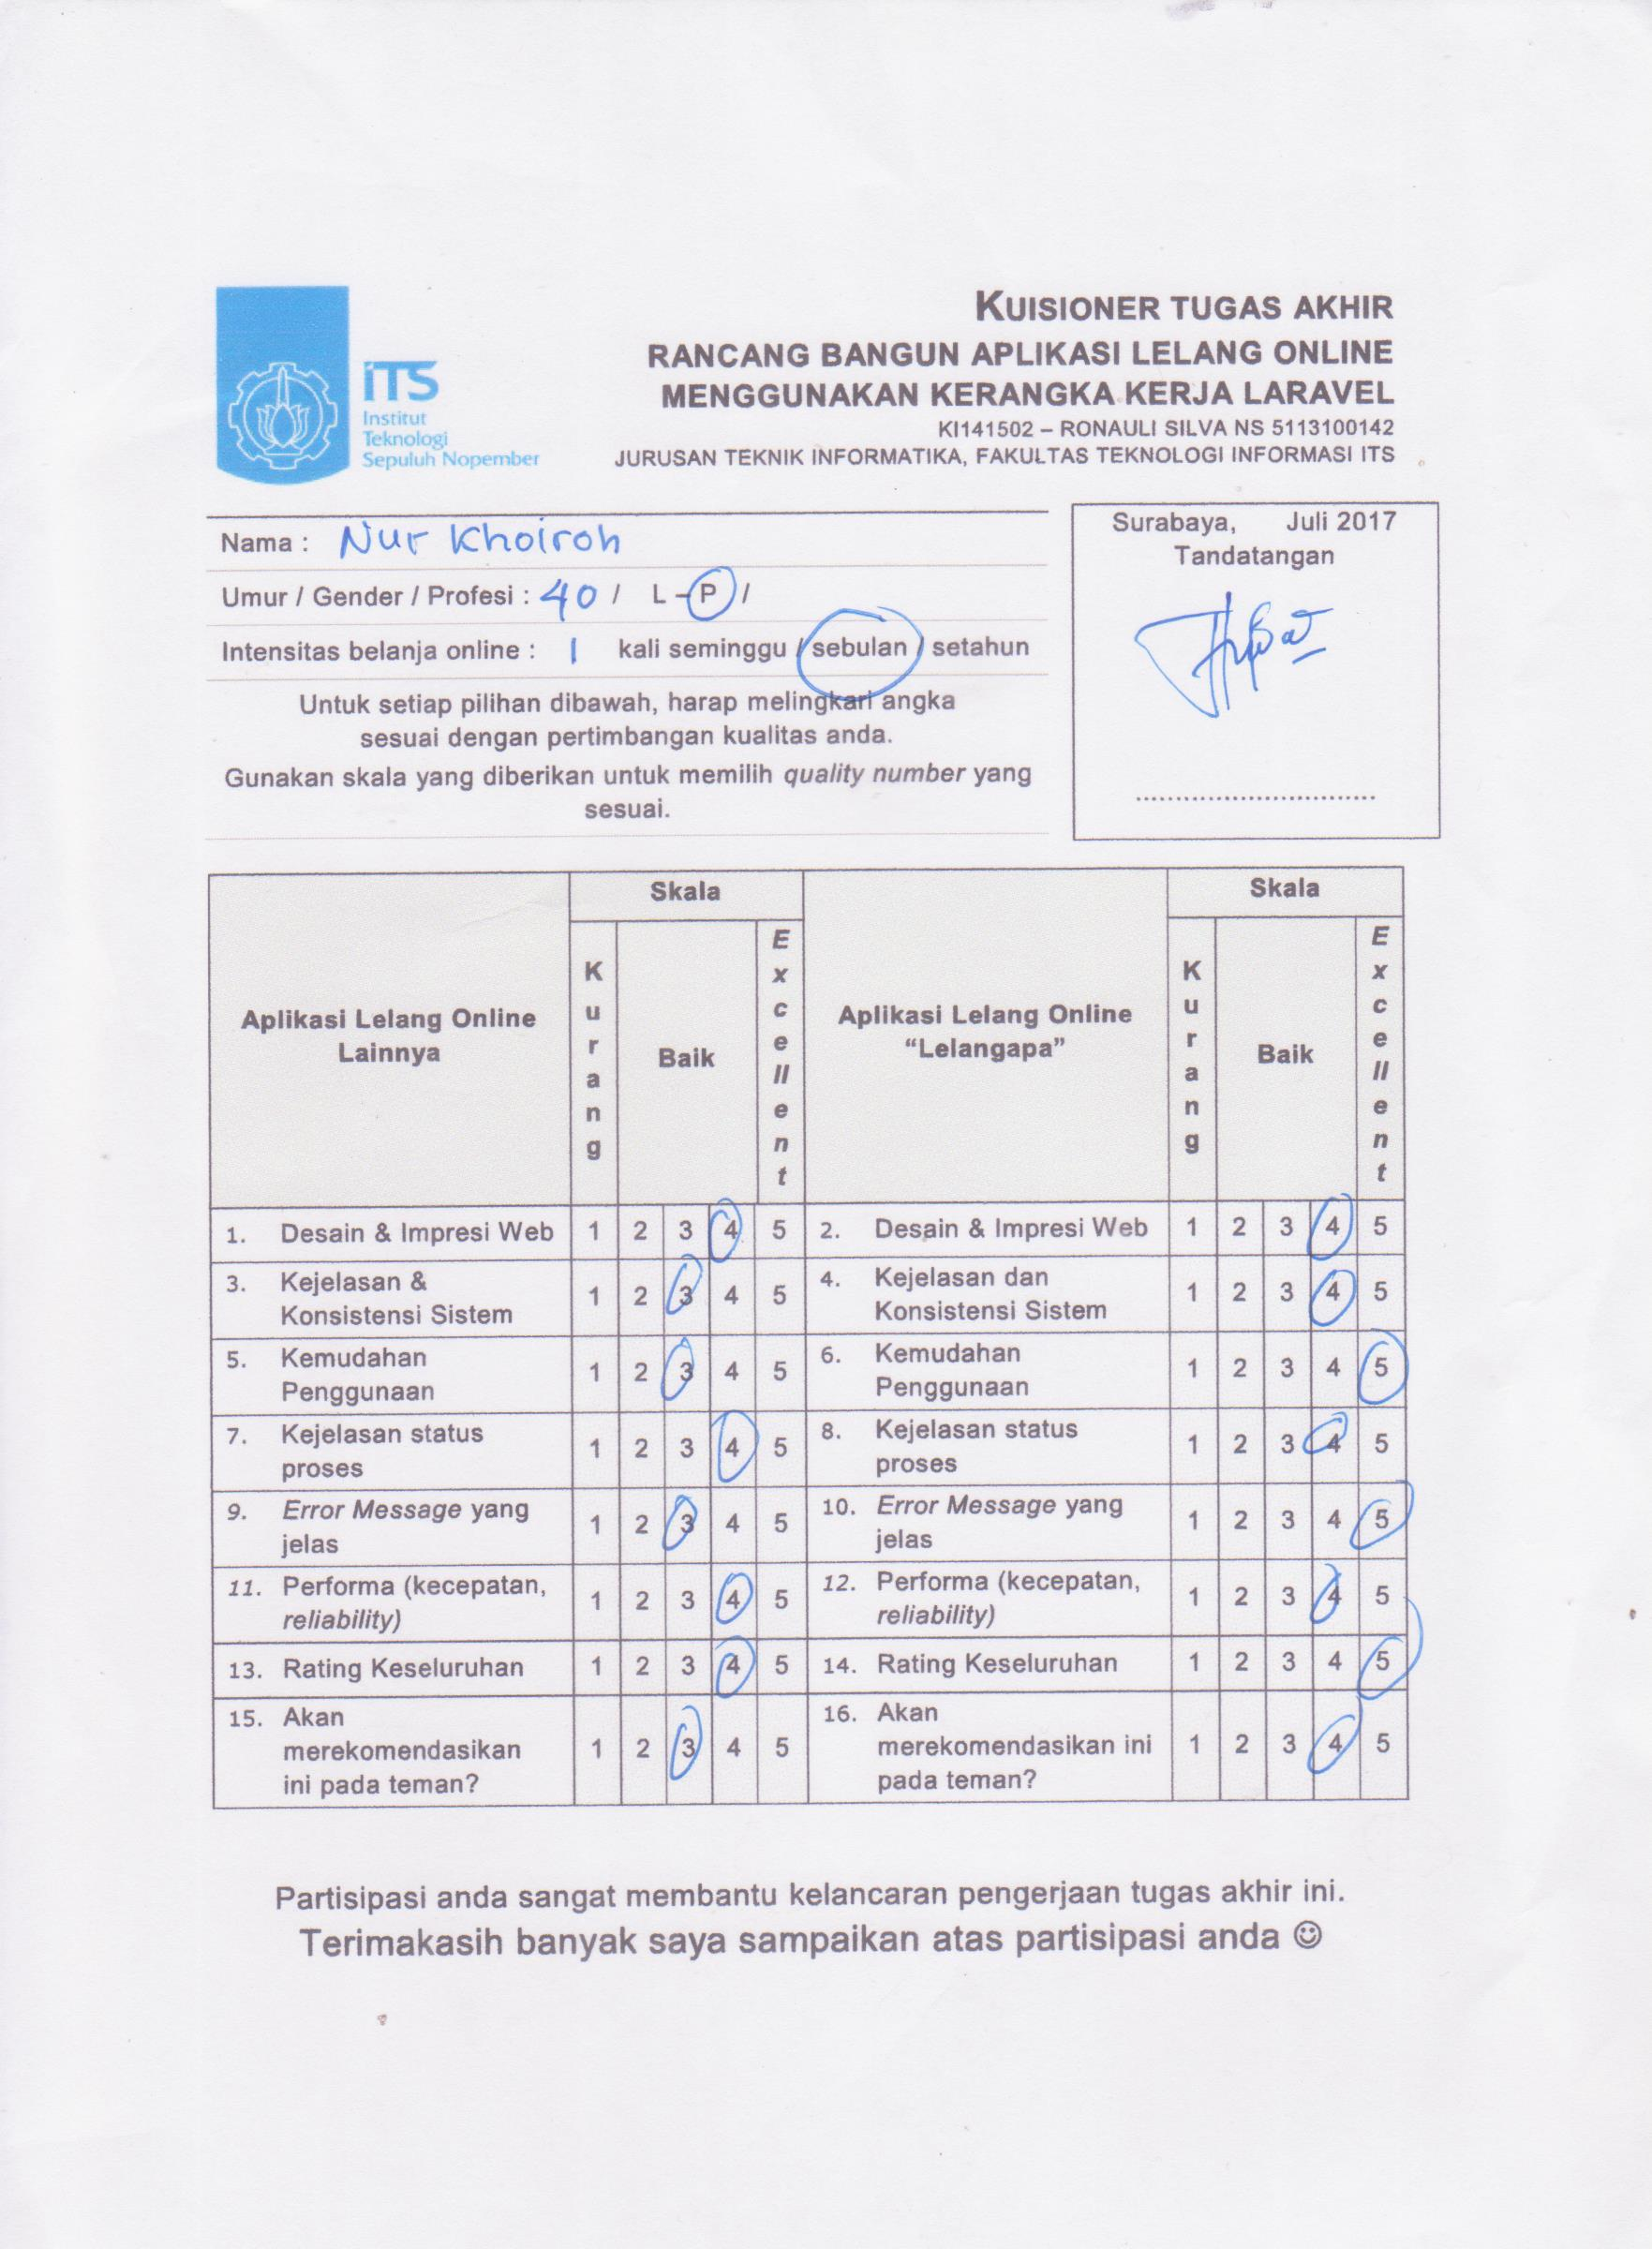
\includegraphics[width=\textwidth]{images/bab5/ujipengguna/5.jpg}
	\caption{Kuisioner Pengguna 5}
	\label{quest-5}
\end{figure}
\begin{figure}[H]
	\centering
	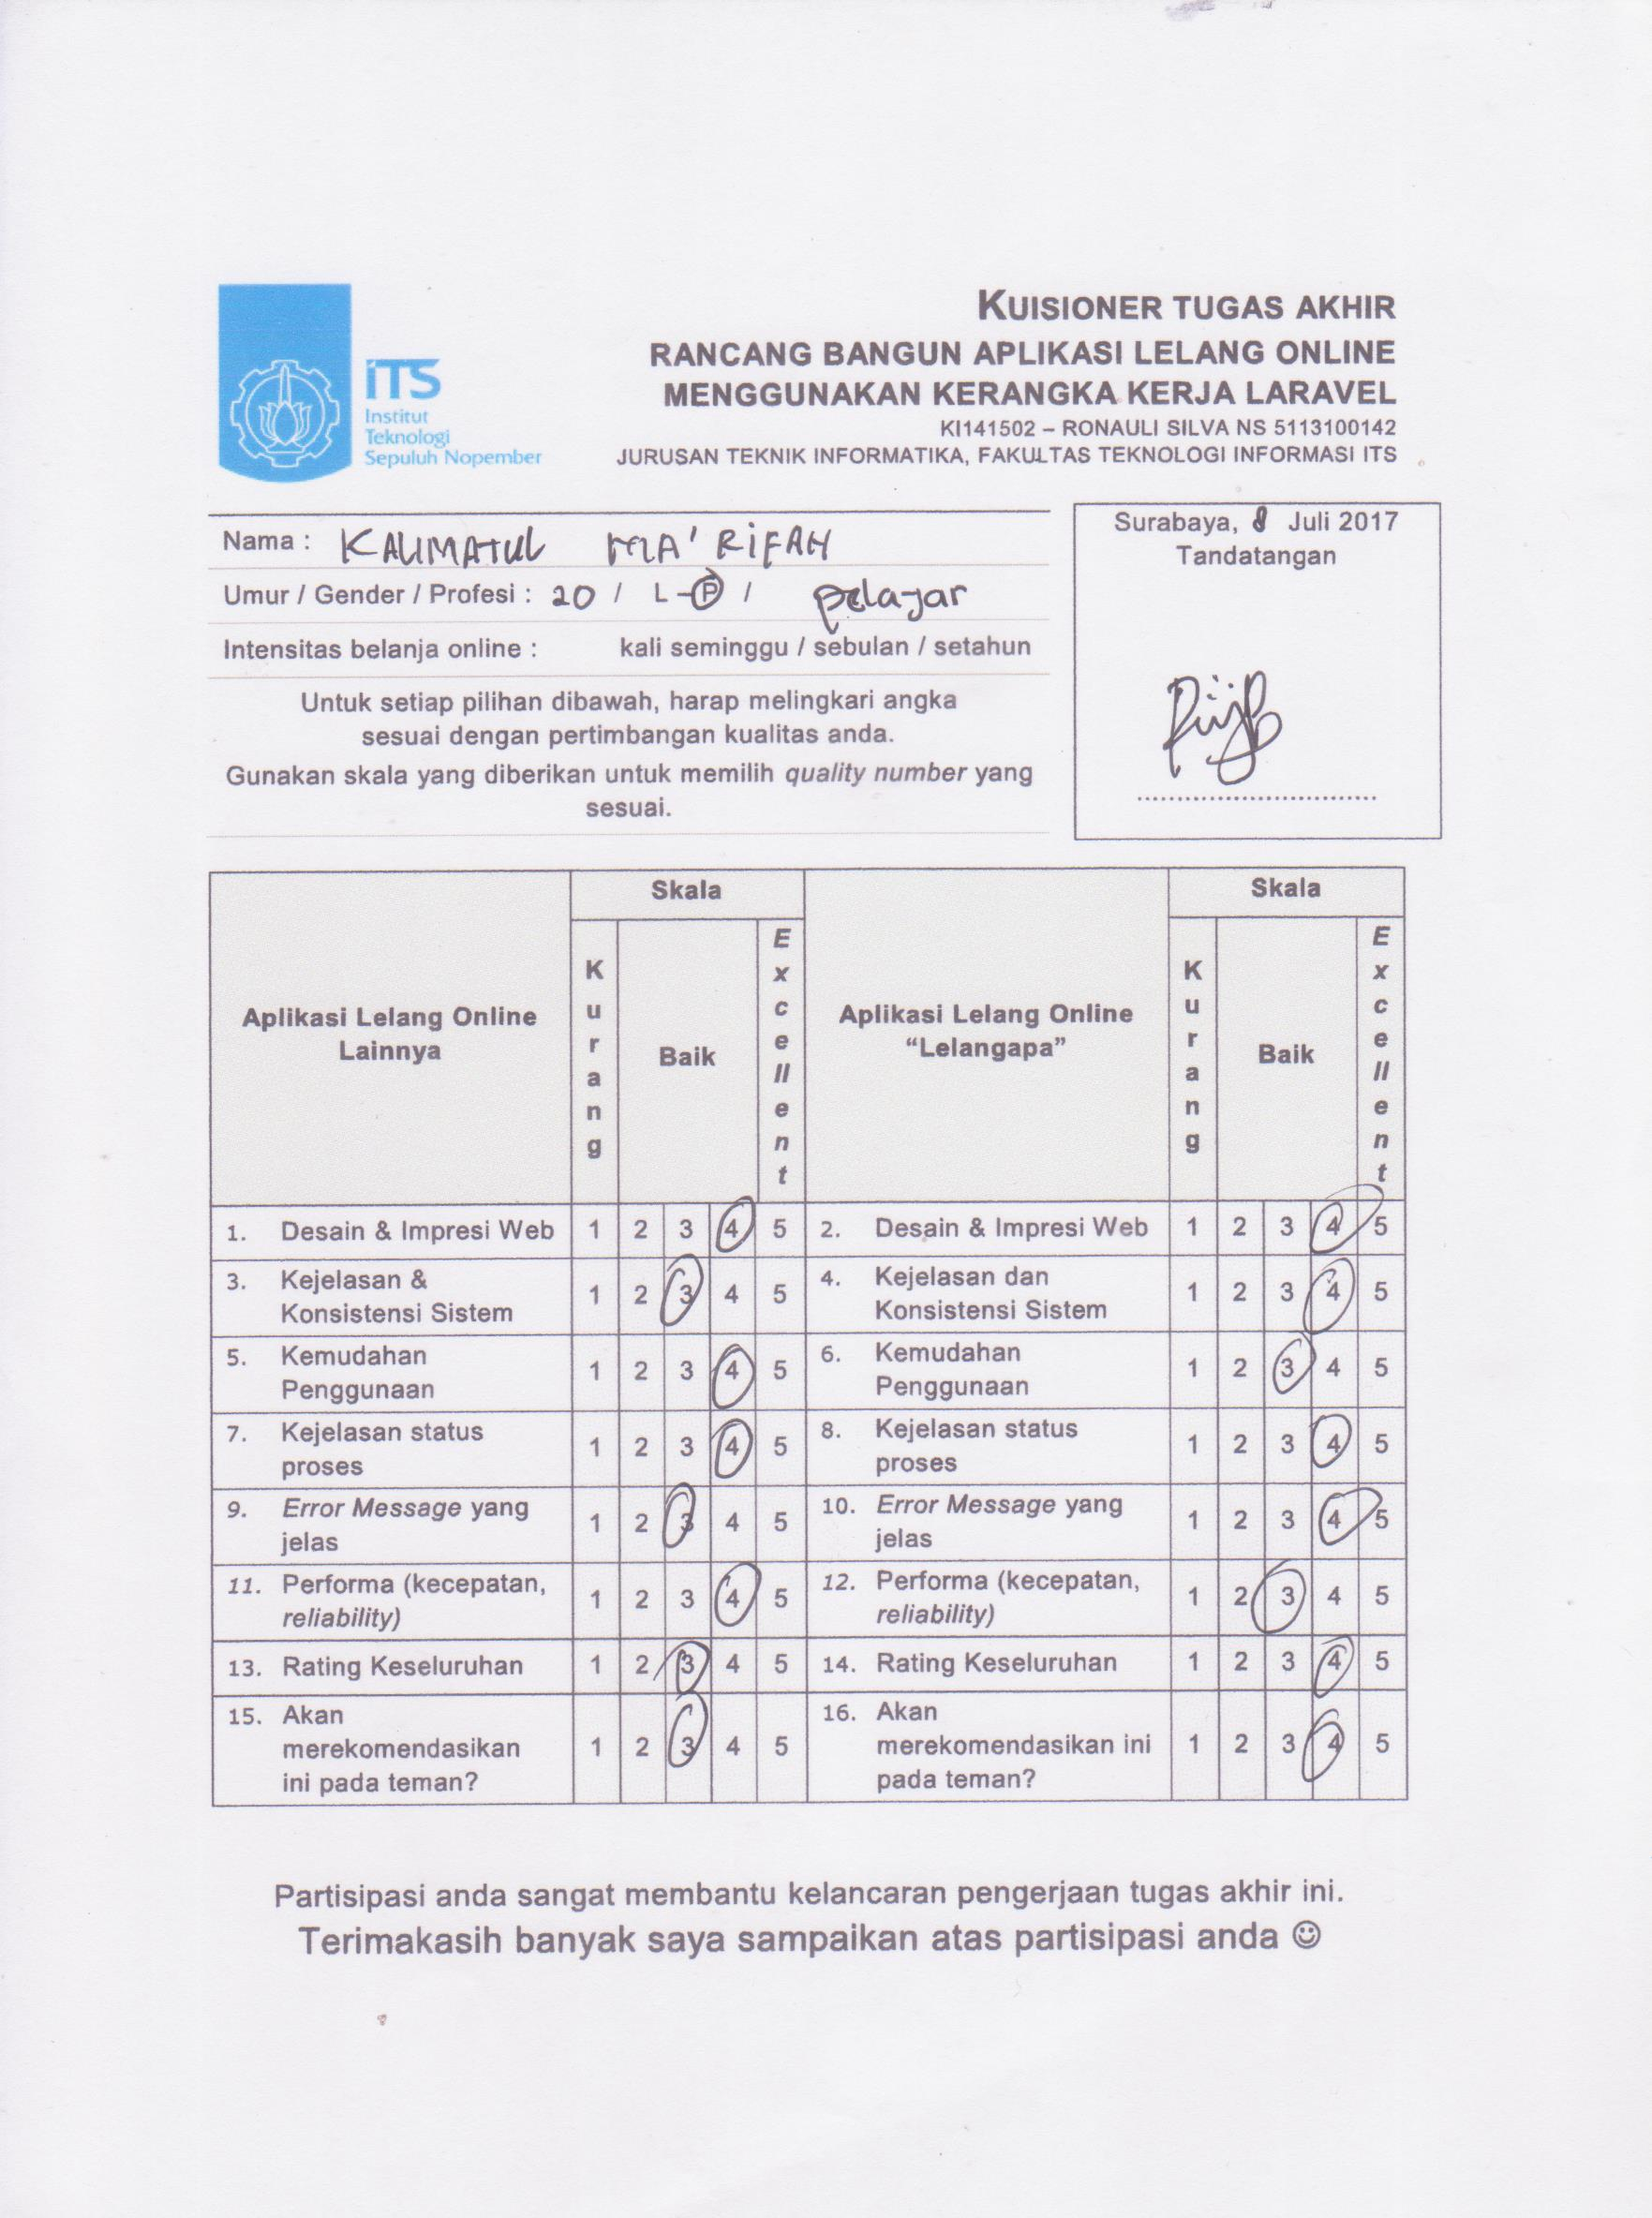
\includegraphics[width=\textwidth]{images/bab5/ujipengguna/6.jpg}
	\caption{Kuisioner Pengguna 6}
	\label{quest-6}
\end{figure}
\begin{figure}[H]
	\centering
	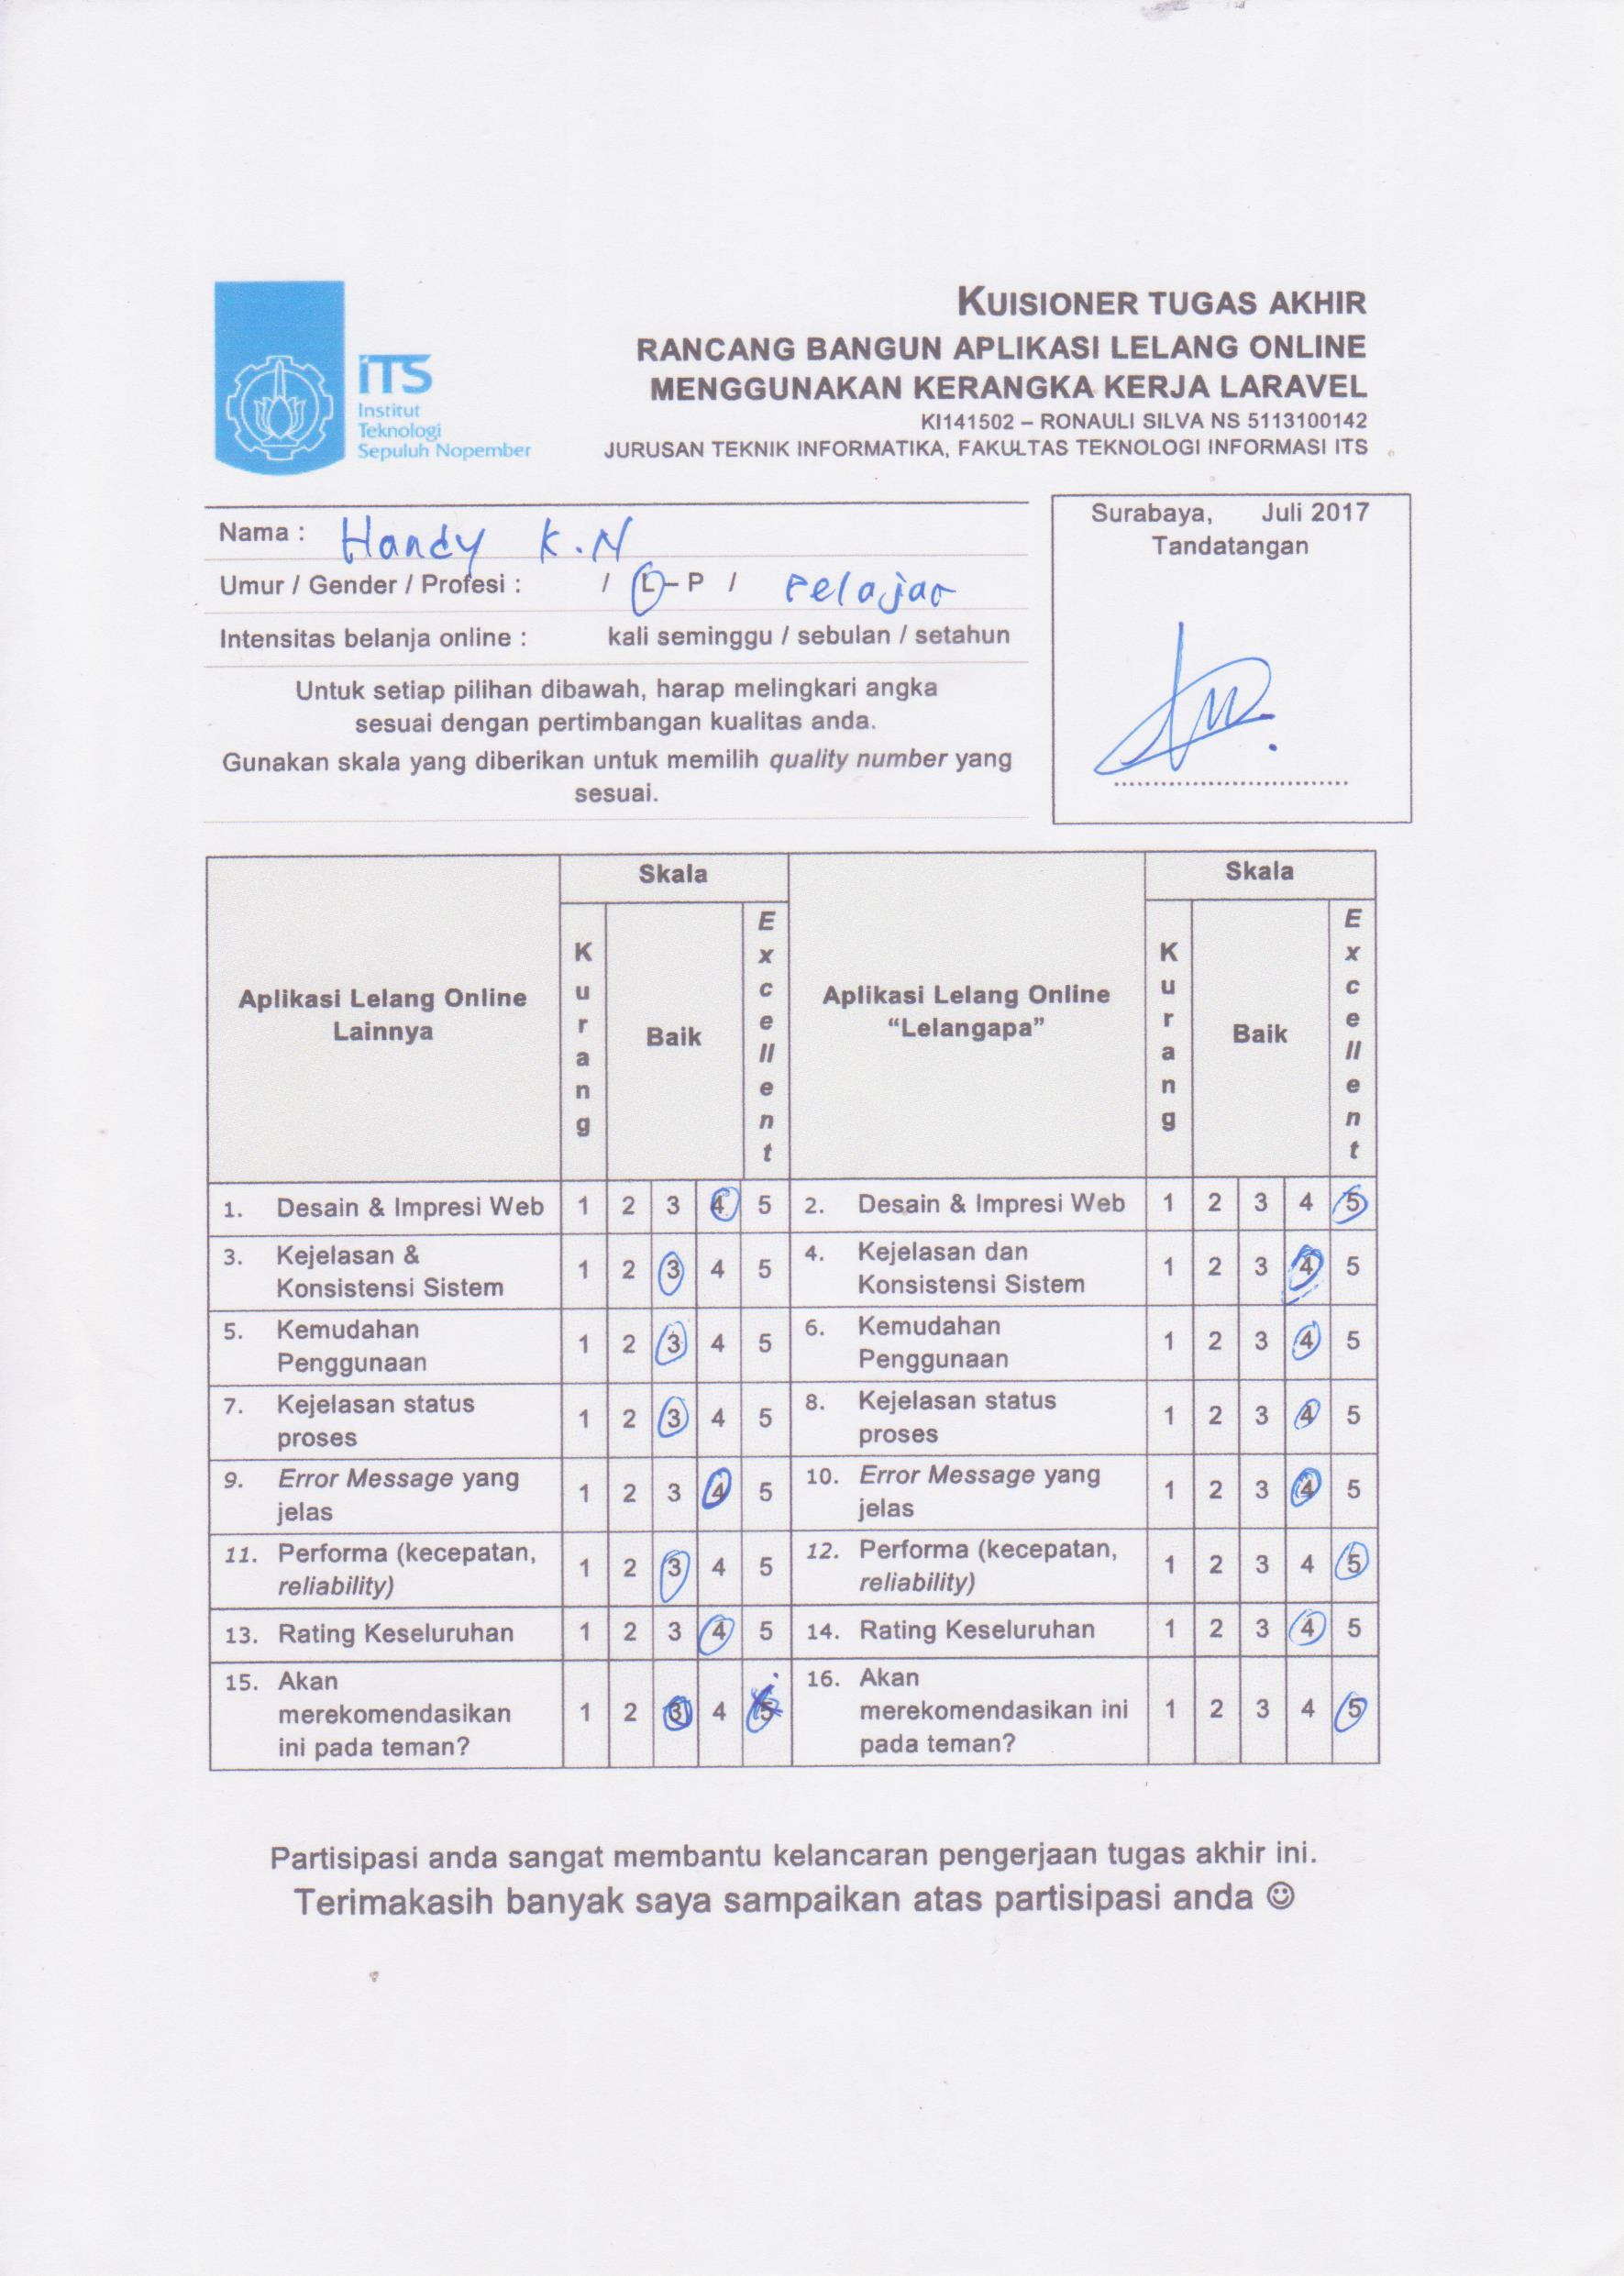
\includegraphics[width=\textwidth]{images/bab5/ujipengguna/7.jpg}
	\caption{Kuisioner Pengguna 1}
	\label{quest-7}
\end{figure}
\begin{figure}[H]
	\centering
	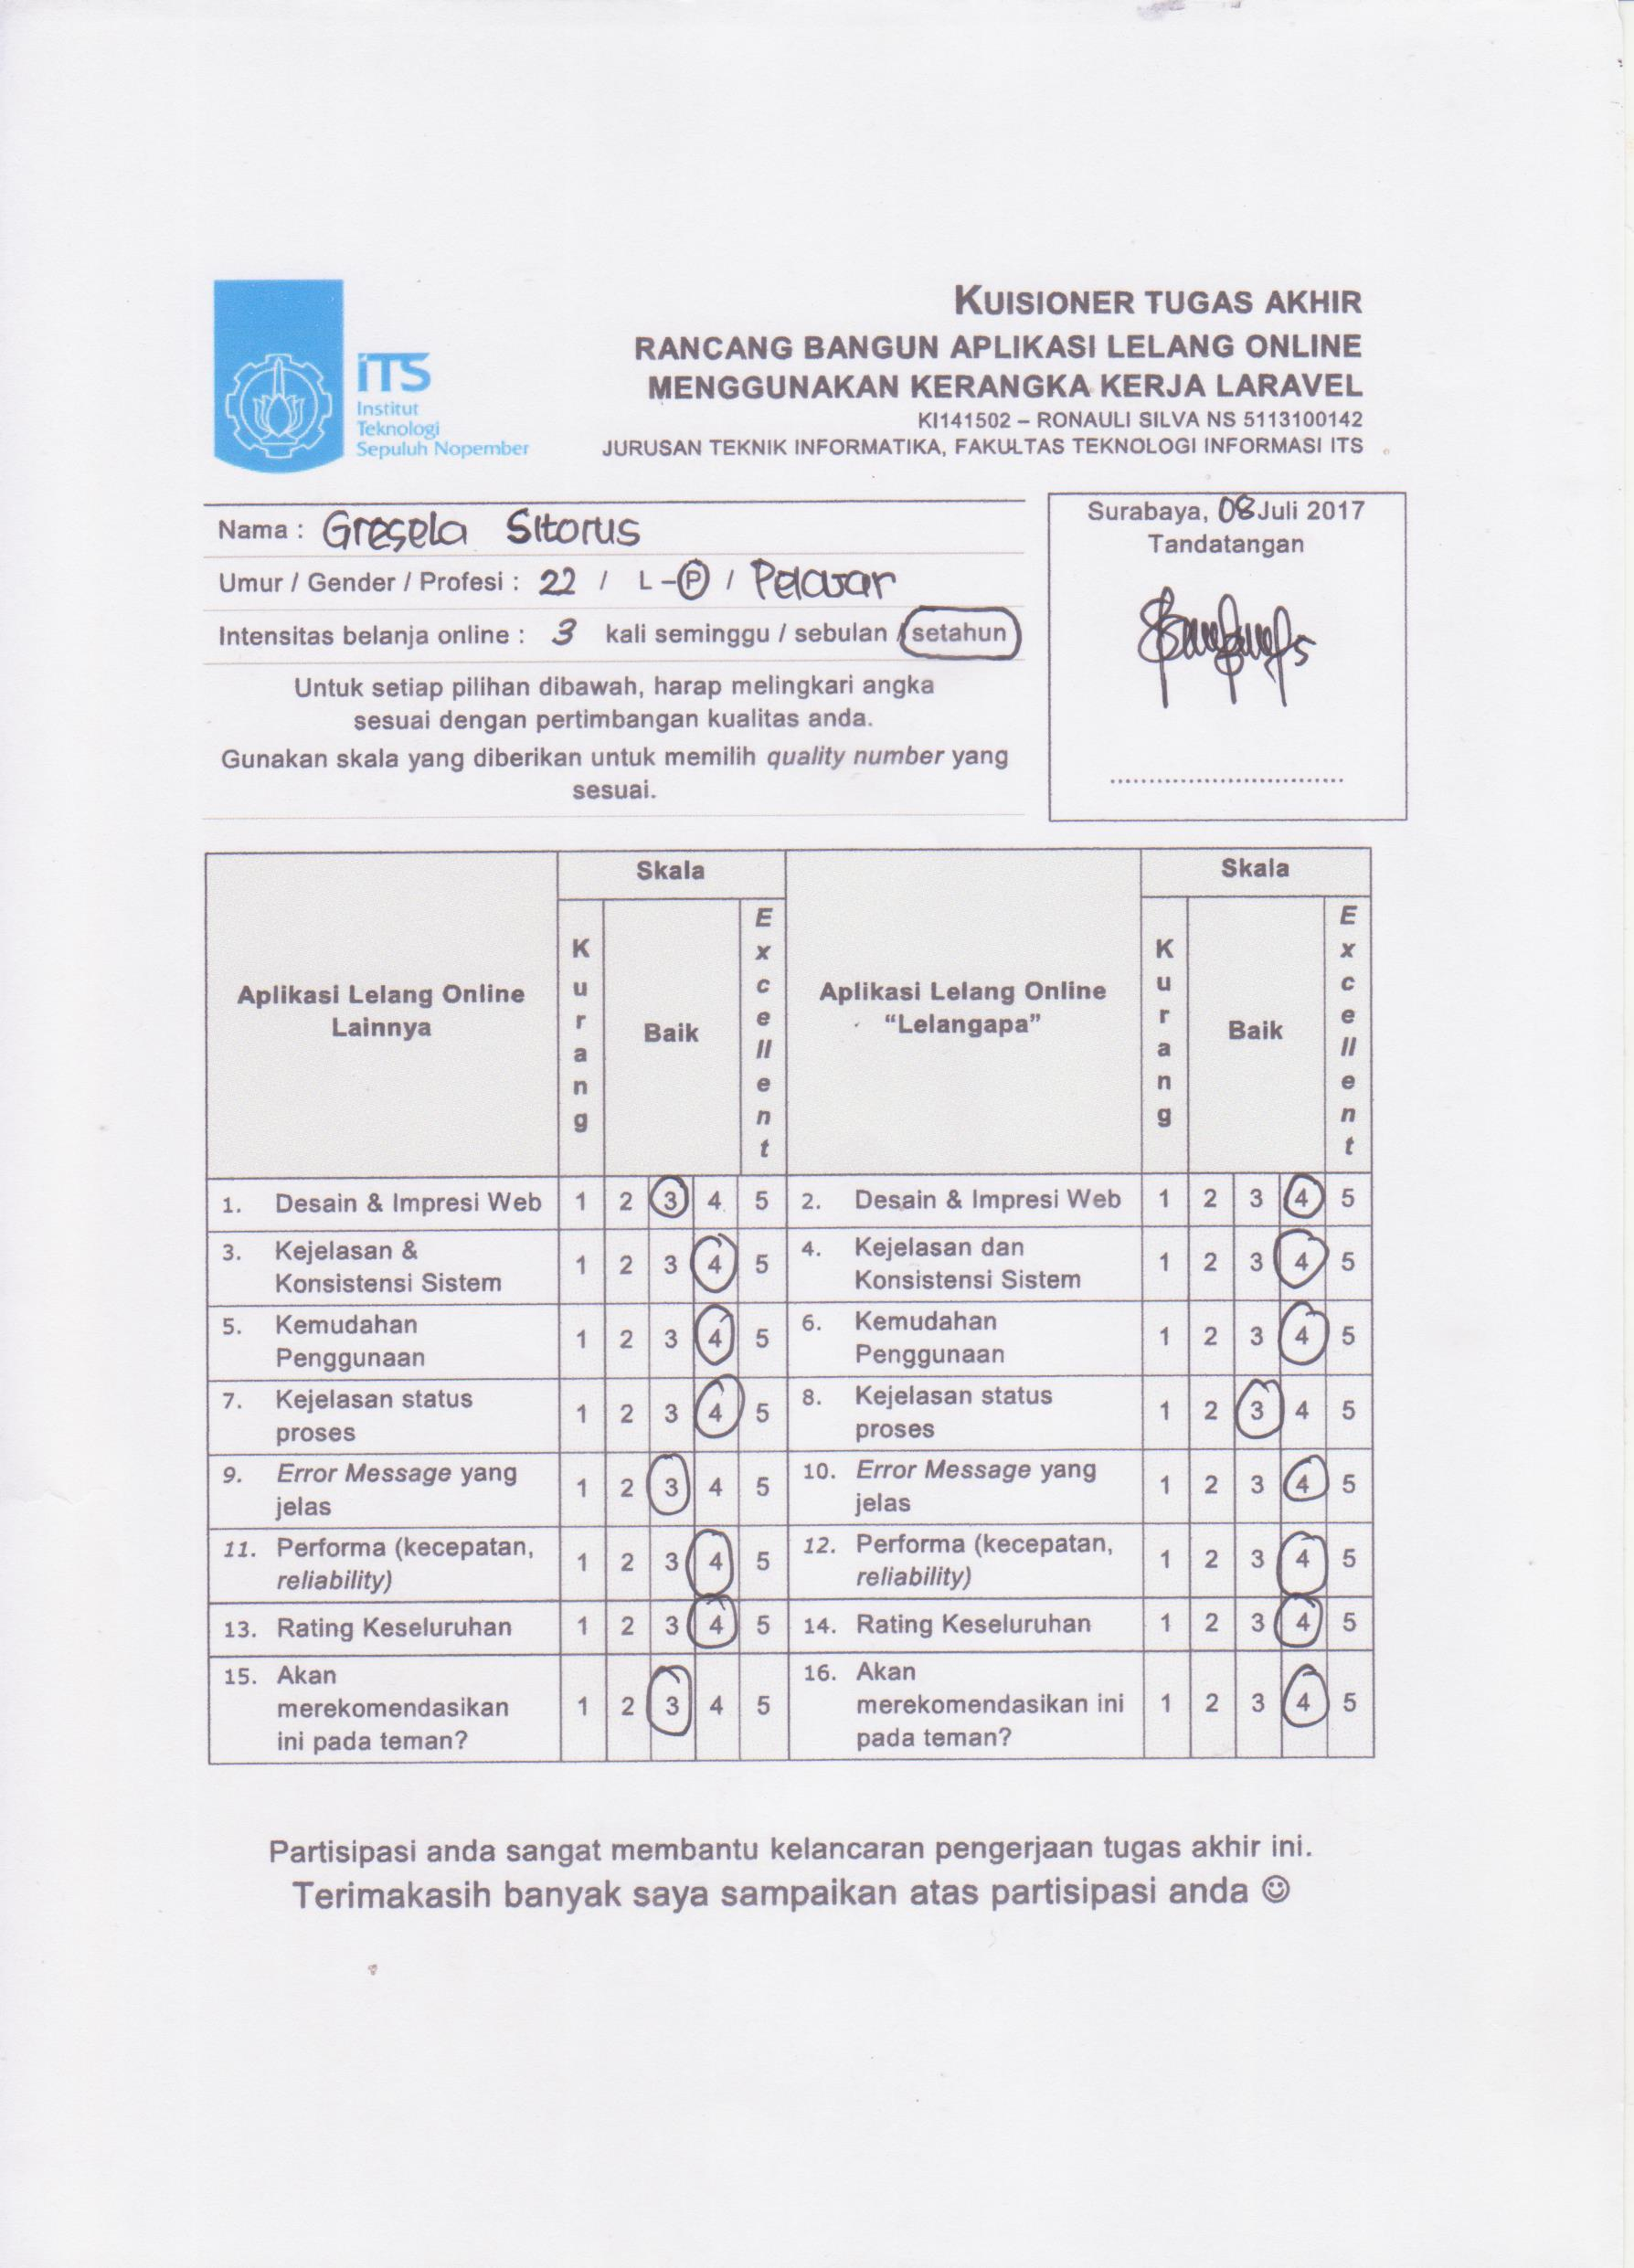
\includegraphics[width=\textwidth]{images/bab5/ujipengguna/8.jpg}
	\caption{Kuisioner Pengguna 8}
	\label{quest-8}
\end{figure}
\begin{figure}[H]
	\centering
	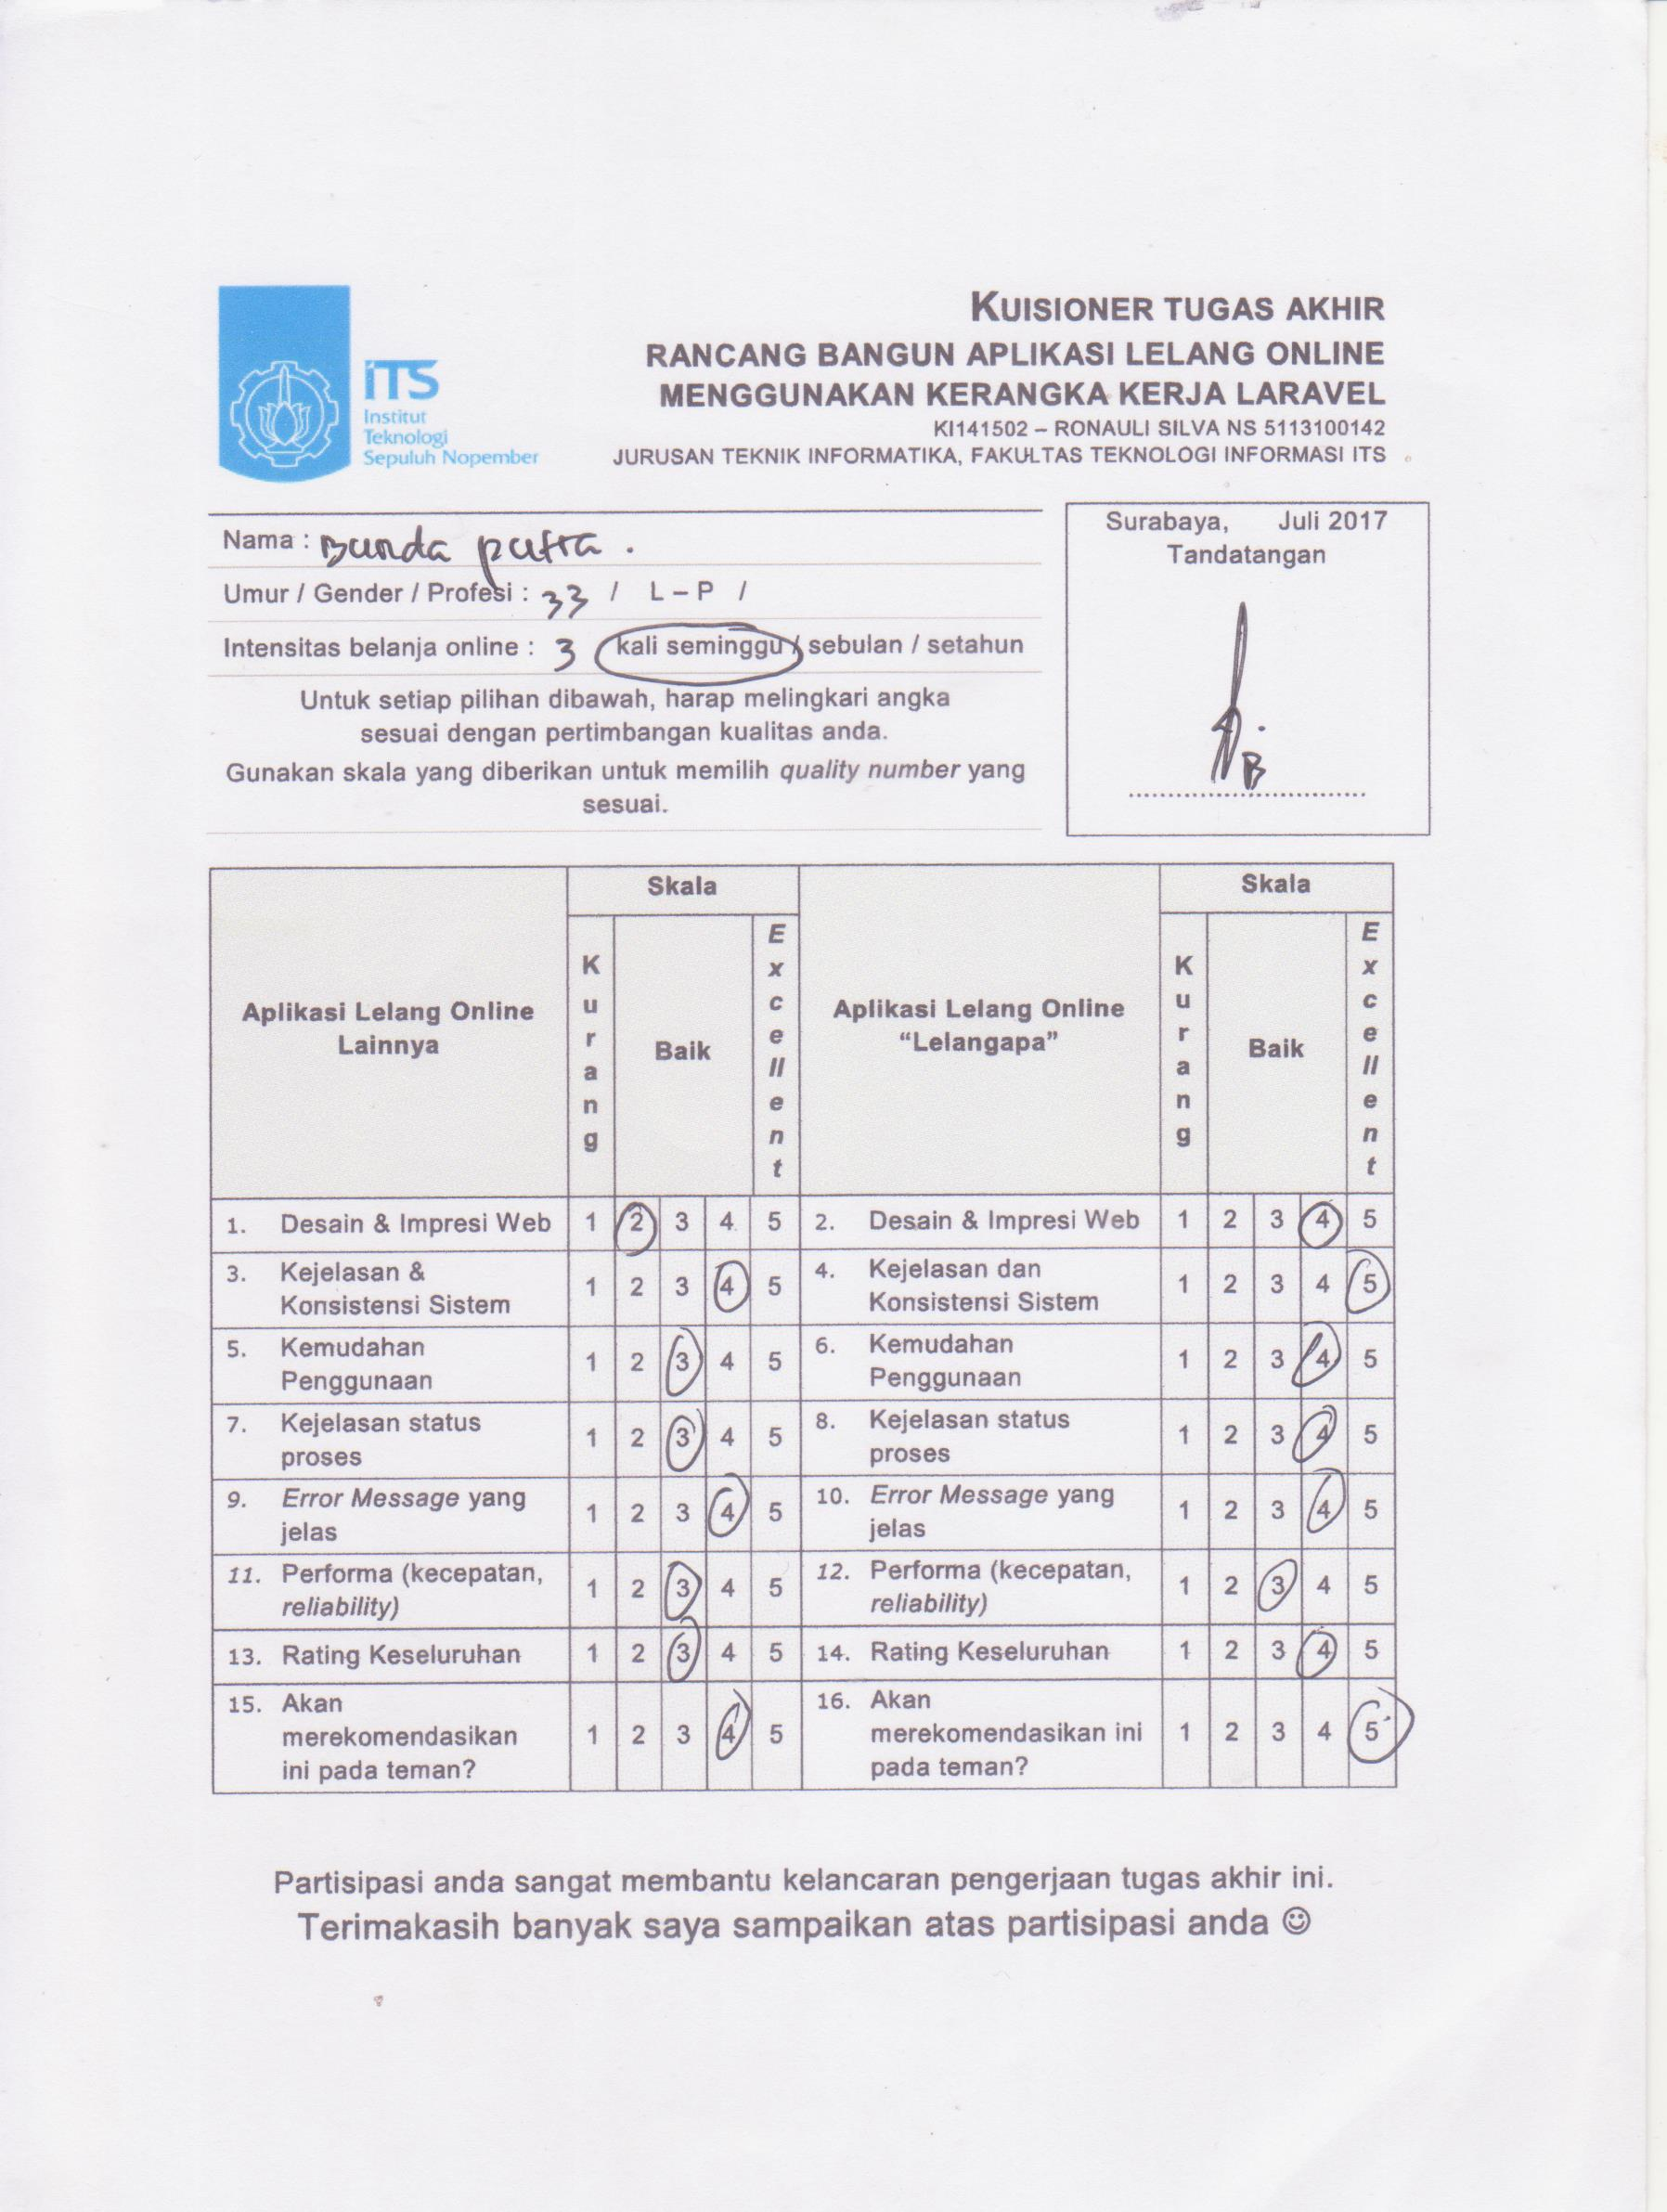
\includegraphics[width=\textwidth]{images/bab5/ujipengguna/9.jpg}
	\caption{Kuisioner Pengguna 9}
	\label{quest-9}
\end{figure}
\begin{figure}[H]
	\centering
	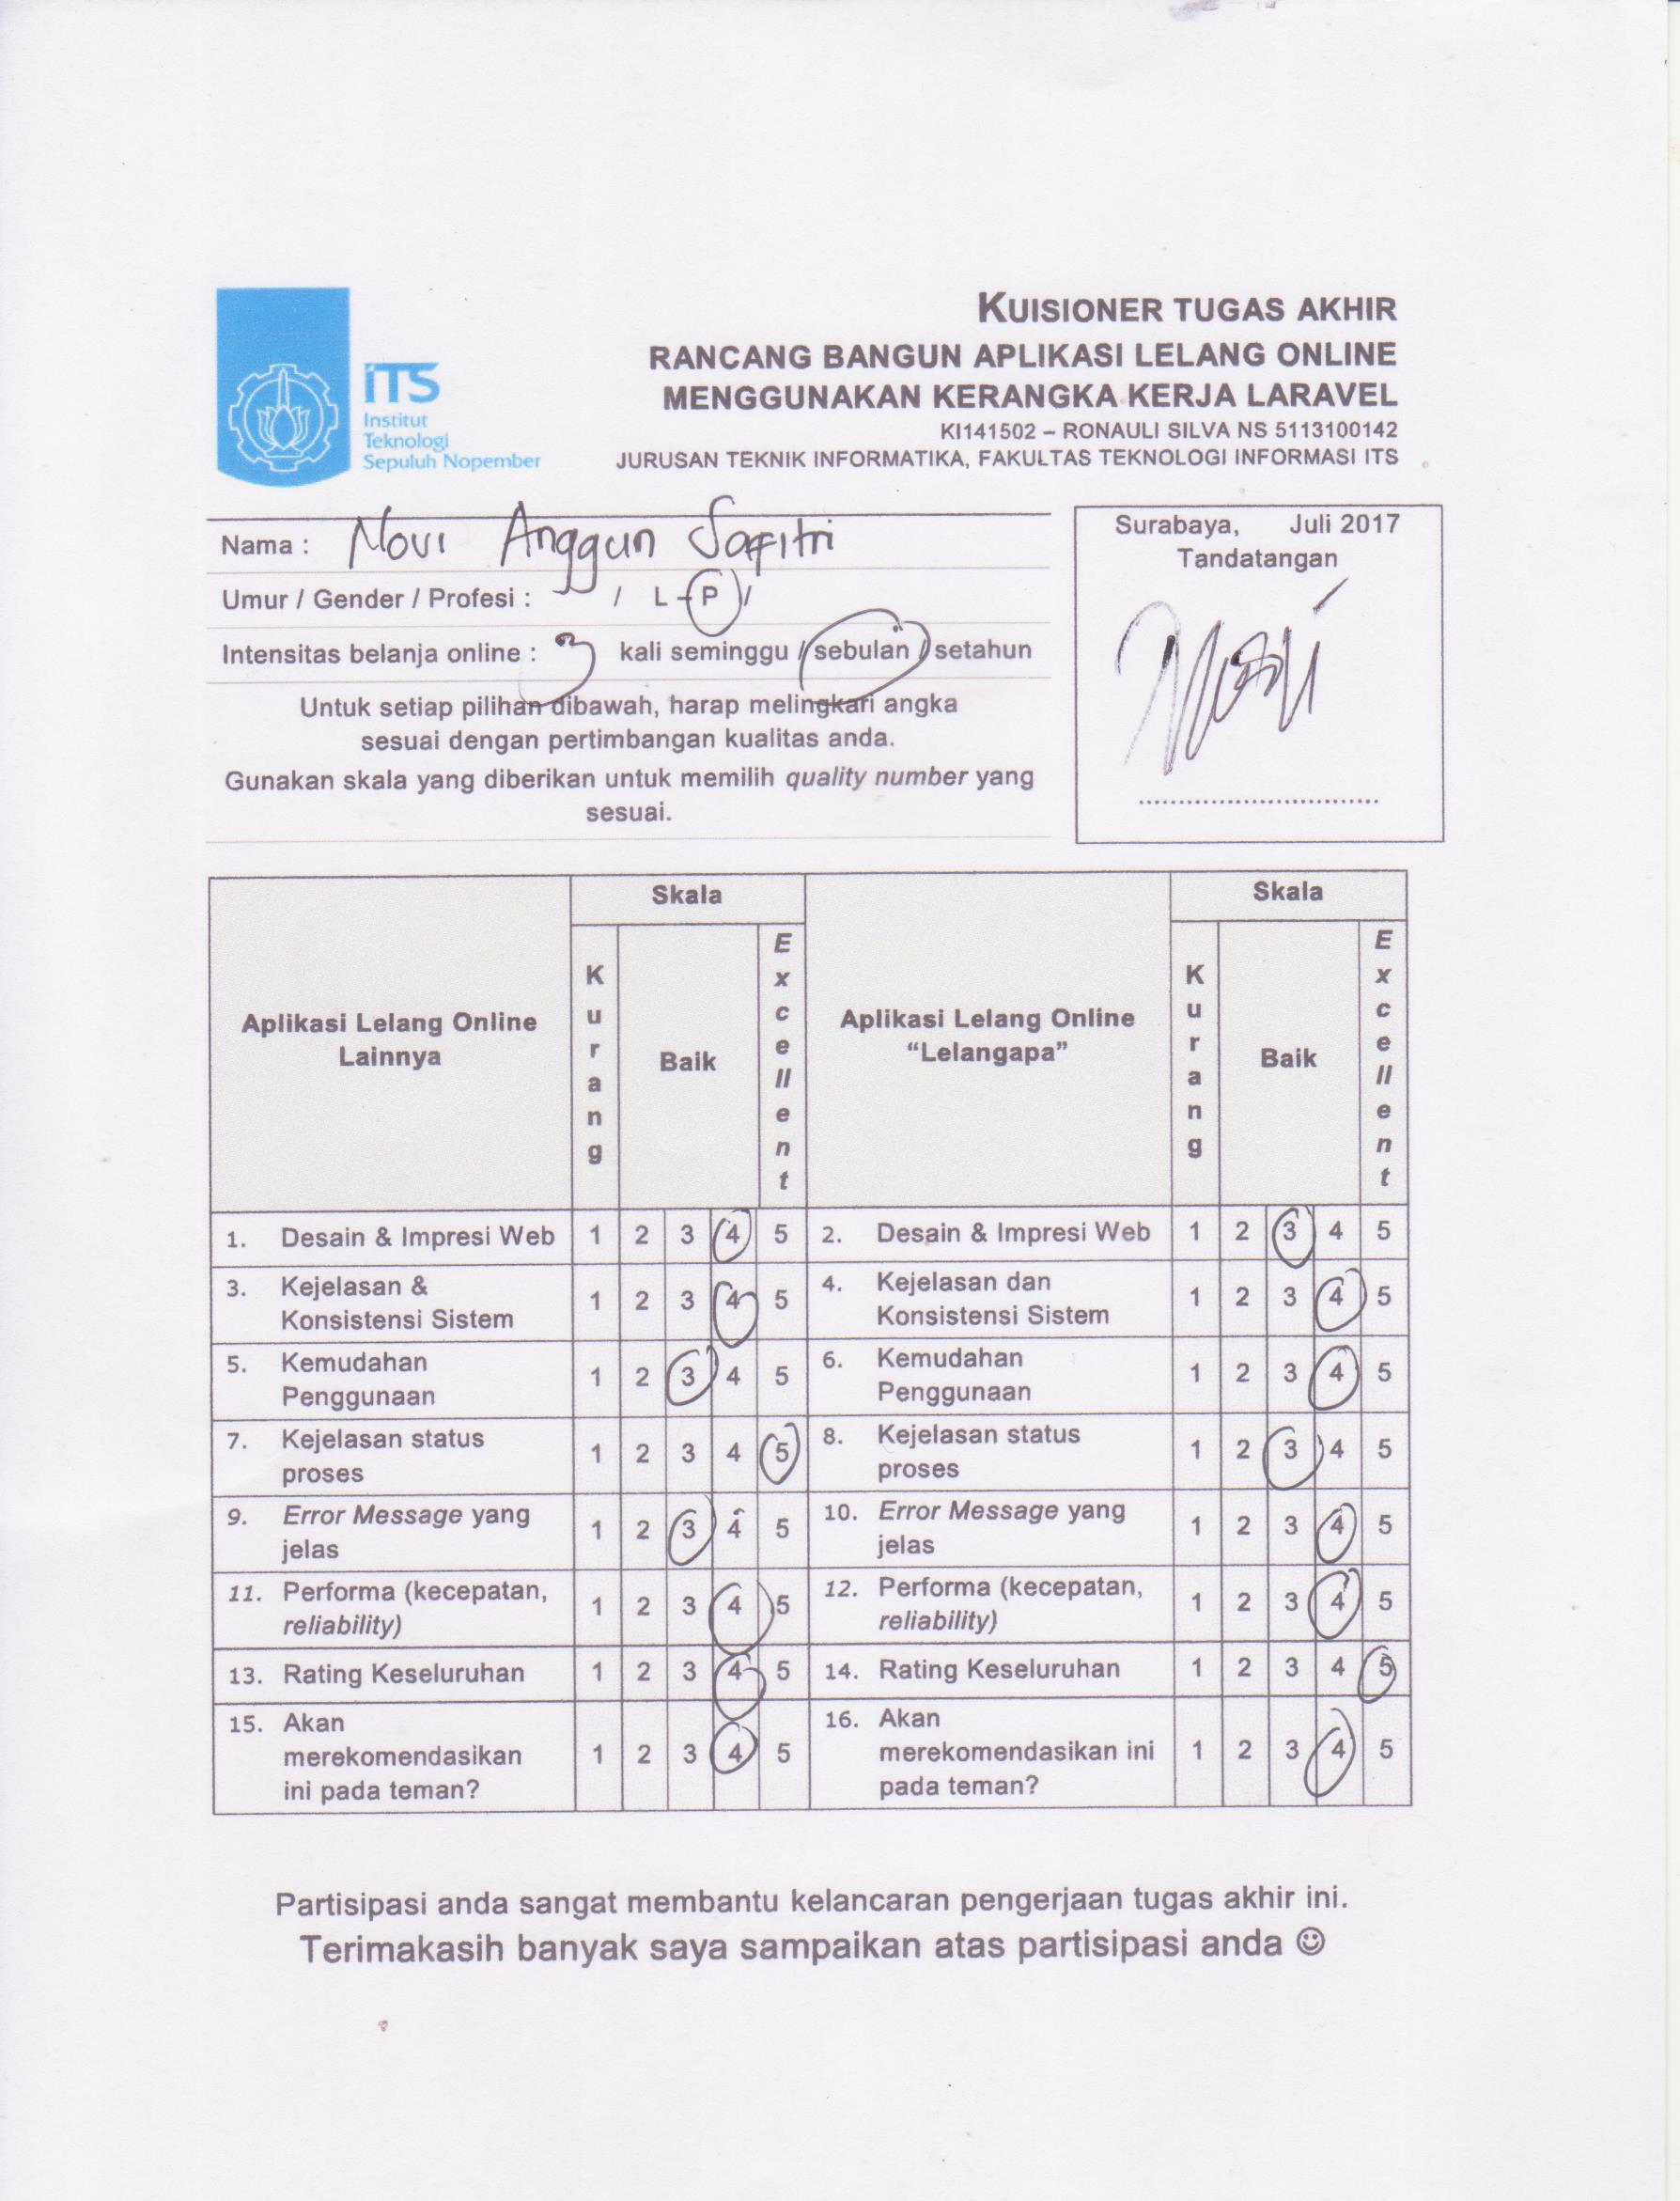
\includegraphics[width=\textwidth]{images/bab5/ujipengguna/10.jpg}
	\caption{Kuisioner Pengguna 10}
	\label{quest-10}
\end{figure}
\begin{figure}[H]
	\centering
	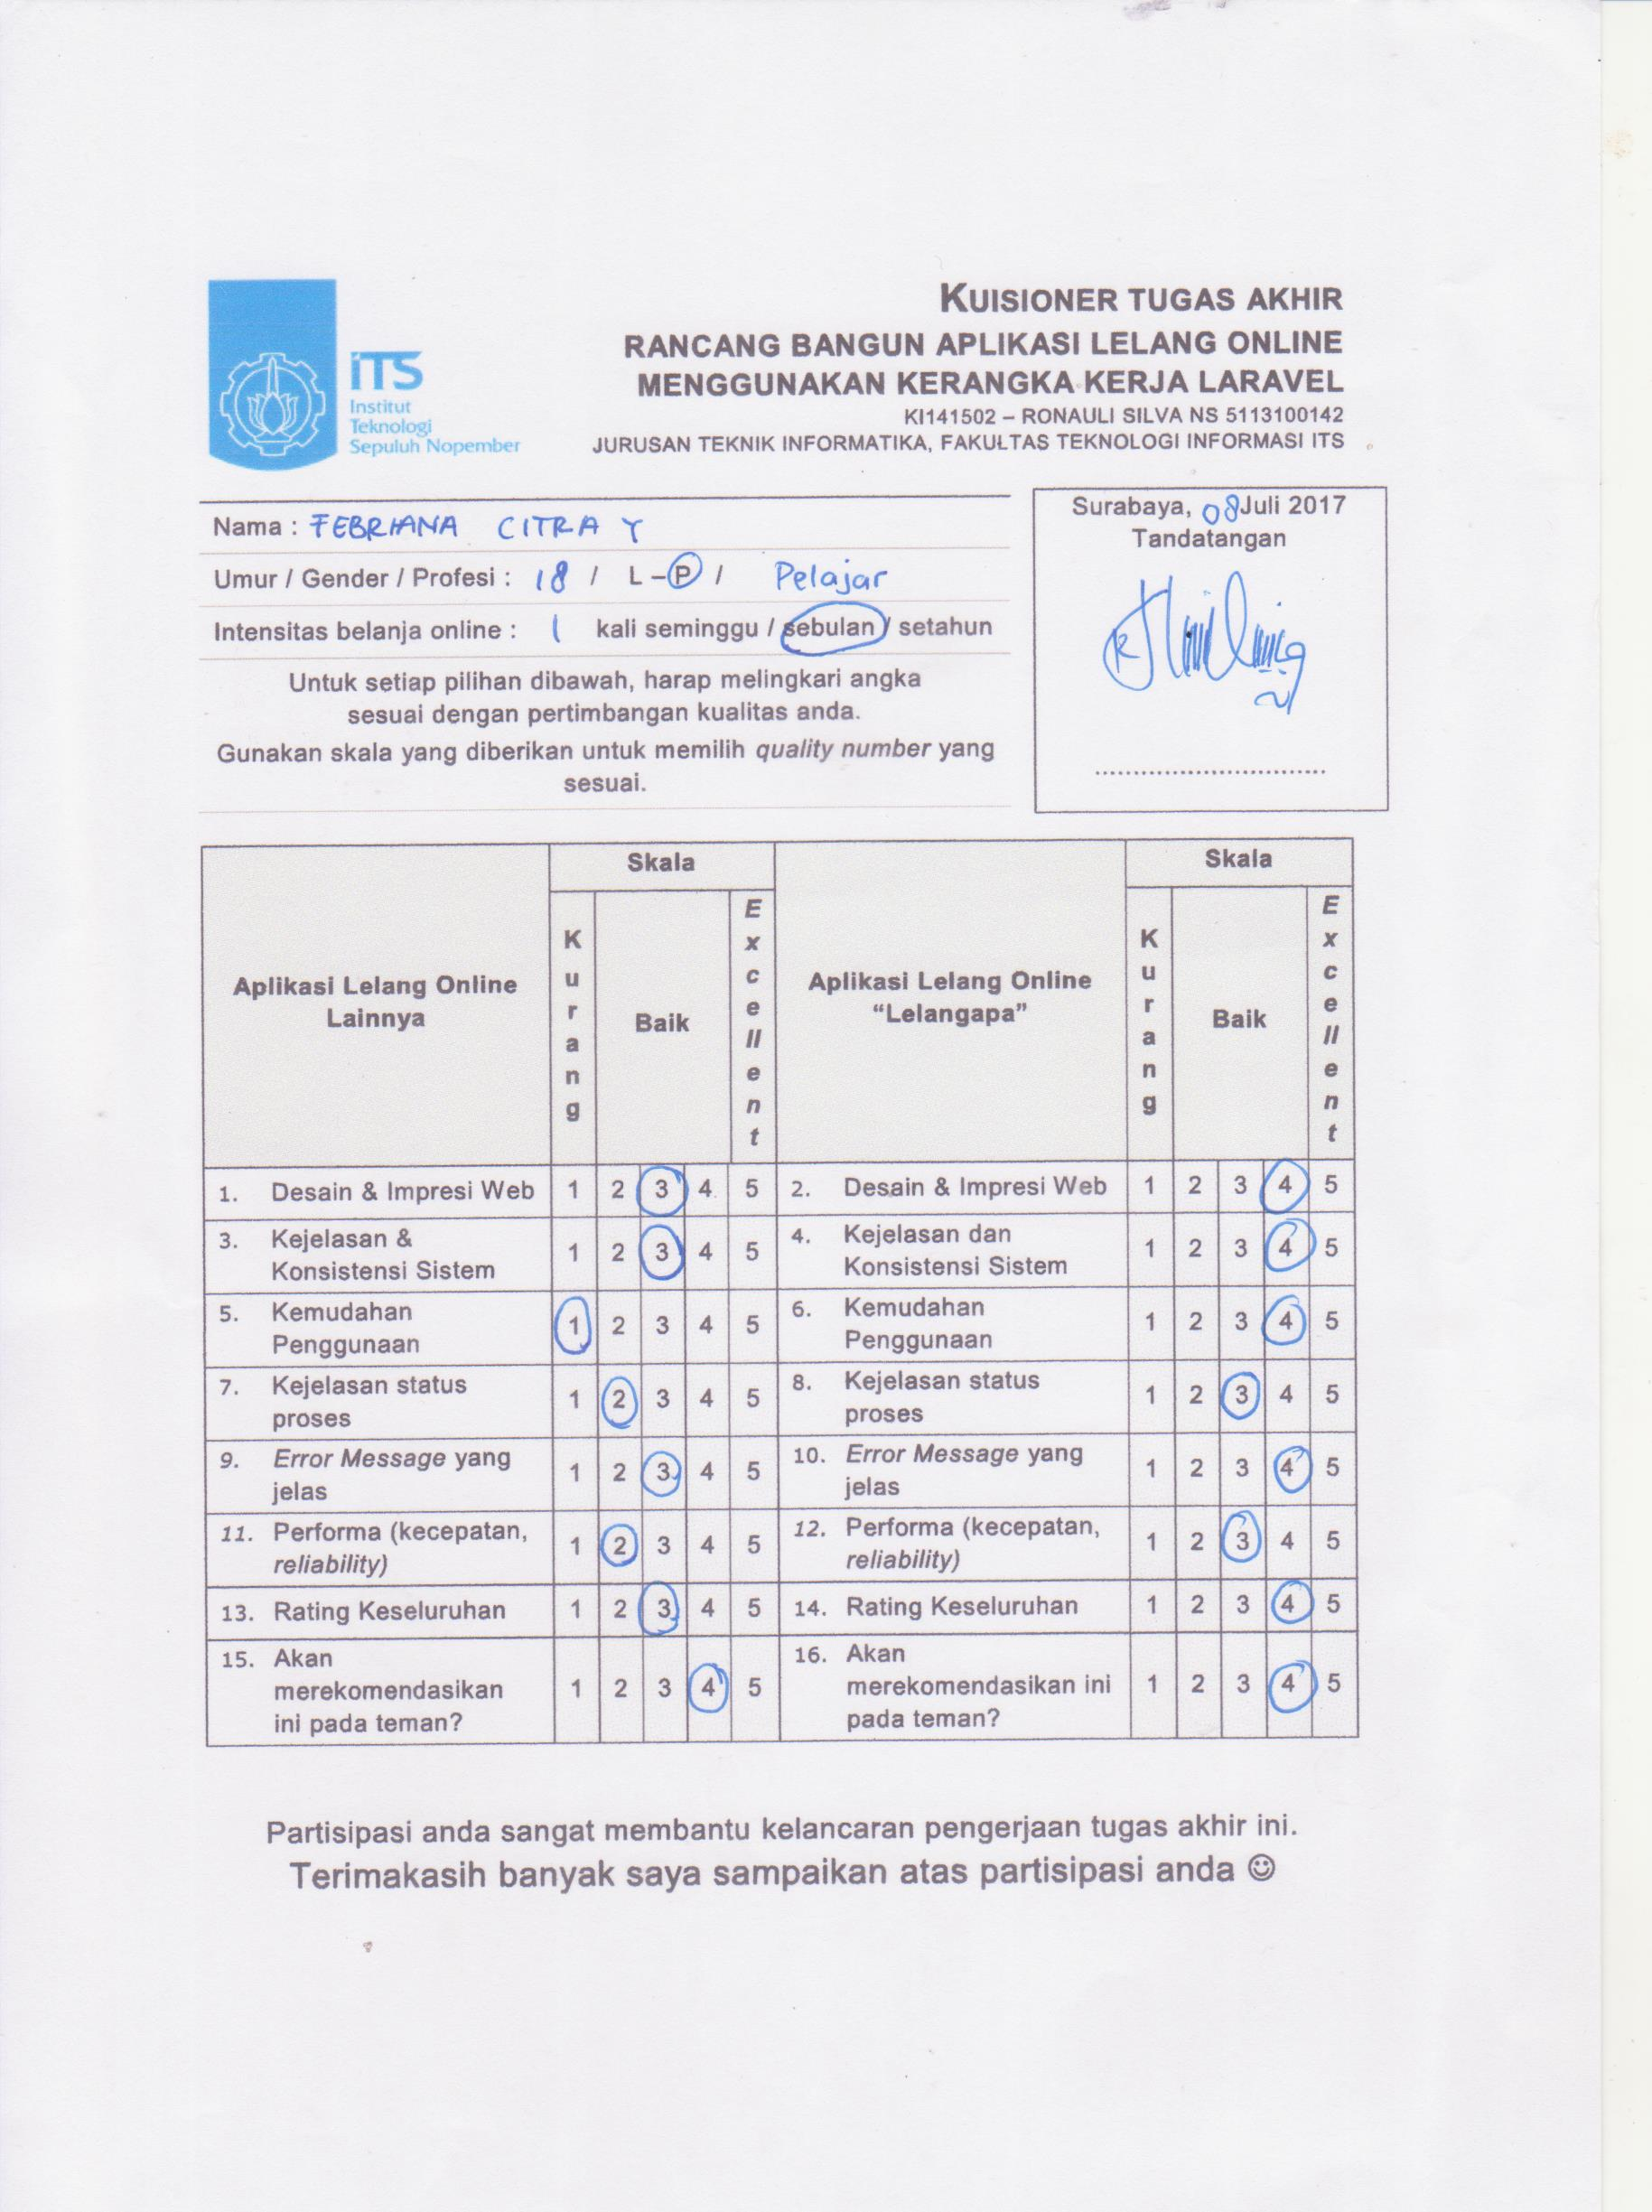
\includegraphics[width=\textwidth]{images/bab5/ujipengguna/11.jpg}
	\caption{Kuisioner Pengguna 11}
	\label{quest-11}
\end{figure}


  \backmatter % Lampiran tanpa judul LAMPIRAN X, untuk BIODATA PENULIS

    \chapter{BIODATA PENULIS}
		\begin{wrapfigure}{l}{0.3\textwidth}
			
\includegraphics[width=0.3\textwidth]{images/foto-diri.jpg}
		\end{wrapfigure}
		\textbf{Ronauli Silva NS}, seorang yang lahiran \& besar di Siantar Medan - Sumatera Utara, sangat suka belajar. Diberi amanah untuk menjadi \textit{administrator} Laboratorium Pemrograman di tahun 2015, penulis belajar banyak mengenai administrasi \textit{server}, rancang bangun aplikasi terutama di bidang web. Selain itu, beberapa \textit{project} yang diambil penulis mengenai rancang bangun aplikasi yang baik dan buruk yang mengajarkan penulis cara memperbaiki, menangkal dan \& mengoptimasinya.\\
		Selain itu, penulis juga banyak belajar \textit{softskills} saat menjabat sebagai Sekretaris Departemen HMTC ITS 2015/2016 (Kabinet Optimasi) dan lewat pelatihan-pelatihan yang diberikan donatur beasiswa saat penulis masih diamanahi sebagai beswan Karya Salemba Empat 2014-2016.\\ \\
		Motto penulis yaitu "\textit{Always go for the extra miles}", membawa penulis mengambil topik tugas akhir ini, dimana penulis dapat menerapkan perbaikan, optimasi dan pelajaran yang penulis petik dari \textit{project-project} sebelumnya, dengan bimbingan dosen-dosen pembimbing penulis yang baik hati. Dalam pendalaman topik tugas akhir ini juga, penulis banyak belajar dan menjadi sangat tertarik mendalami \textit{bussiness engineering}, \textit{user experiences and usability}, dan \textit{data scientist \& engineering}. \\ \\
		Dengan segala kerendahan hati, ilmu penulis masihlah setitik dibandingkan susu sebelanga. Penulis sangat mengharapkan diskusi, ajaran dan bantuan dalam memperbaiki diri. Apabila pembaca berkenan, penulis dapat dihubungi melalui \textit{email} ke \texttt{ronayumik@gmail.com}, atau \textit{Whatsapp} ke nomor +62821-6066-5568.



\end{document}